% Format teze zasnovan je na paketu memoir
% http://tug.ctan.org/macros/latex/contrib/memoir/memman.pdf ili
% http://texdoc.net/texmf-dist/doc/latex/memoir/memman.pdf
% 
% Prilikom zadavanja klase memoir, navedenim opcijama se podešava 
% veličina slova (12pt) i jednostrano štampanje (oneside).
% Ove parametre možete menjati samo ako pravite nezvanične verzije
% mastera za privatnu upotrebu (na primer, u b5 varijanti ima smisla 
% smanjiti 
\documentclass[11pt,oneside]{memoir}

% Paket koji definiše sve specifičnosti mastera Matematičkog fakulteta
\usepackage{matfmaster}
\usepackage{amsmath}
\usepackage{float}
\usepackage{xcolor}
\usepackage[normalem]{ulem}
\usepackage{pythonhighlight}
\usepackage{subcaption}

\DeclareMathOperator*{\argmax}{arg\,max}
\DeclareMathOperator*{\argmin}{arg\,min}
%
% Podrazumevano pismo je ćirilica.
%   Ako koristite pdflatex, a ne xetex, sav latinički tekst na srpskom jeziku
%   treba biti okružen sa \lat{...} ili \begin{latinica}...\end{latinica}.
%
% Opicija [latinica]:
%   ako želite da pišete latiniciom, dodajte opciju "latinica" tj.
%   prethodni paket uključite pomoću: \usepackage[latinica]{matfmaster}.
%   Ako koristite pdflatex, a ne xetex, sav ćirilički tekst treba biti
%   okružen sa \cir{...} ili \begin{cirilica}...\end{cirilica}.
%
% Opcija [biblatex]:
%   ako želite da koristite reference na više jezika i umesto paketa
%   bibtex da koristite BibLaTeX/Biber, dodajte opciju "biblatex" tj.
%   prethodni paket uključite pomoću: \usepackage[biblatex]{matfmaster}
%
% Opcija [b5paper]:
%   ako želite da napravite verziju teze u manjem (b5) formatu, navedite
%   opciju "b5paper", tj. prethodni paket uključite pomoću: 
%   \usepackage[b5paper]{matfmaster}. Tada ima smisla razmisliti o promeni
%   veličine slova (izmenom opcije 12pt na 11pt u \documentclass{memoir}).
%
% Naravno, opcije je moguće kombinovati.
% Npr. \usepackage[b5paper,biblatex]{matfmaster}

% Pomoćni paket koji generiše nasumičan tekst u kojem se javljaju sva slova
% azbuke (nema potrebe koristiti ovo u pravim disertacijama)
\usepackage{pangrami}

% Paket koji obezbeđuje ispravni prikaz ćiriličkih italik slova kada
% se koristi pdflatex. Zakomentarisati ako na sistemu koji koristite ovaj
% paket nije dostupan ili ako ne radi ispravno.
\usepackage{cmsrb}

% Ostali paketi koji se koriste u dokumentu
\usepackage{listings} % listing programskog koda
\usepackage{hyperref}

% Ime kandidata na srpskom jeziku (u odabranom pismu)
\autor{Момир Аџемовић}
% Naslov teze na srpskom jeziku (u odabranom pismu)
\naslov{Предвиђање траjекториjа више обjеката на сцени}
% Godina u kojoj je teza predana komisiji
\godina{2022}
% Ime i afilijacija mentora (u odabranom pismu)
\mentor{др Младен Николић, ванредни професор\\ Универзитет у Београду, Математички факултет}
% Ime i afilijacija prvog člana komisije (u odabranom pismu)
\komisijaA{др Јована Ковачевић, доцент\\ Универзитет у Београду, Математички факултет}
% Ime i afilijacija drugog člana komisije (u odabranom pismu)
\komisijaB{др Александар Картељ, доцент\\ Универзитет у Београду, Математички факултет}
% Ime i afilijacija trećeg člana komisije (opciono)
% \komisijaC{}
% Ime i afilijacija četvrtog člana komisije (opciono)
% \komisijaD{}
% Datum odbrane (obrisati ili iskomentarisati narednu liniju ako datum odbrane nije poznat)
\datumodbrane{15. септембар 2022.}

% Apstrakt na srpskom jeziku (u odabranom pismu)
\apstr{%
Циљ рада jе анализа постоjећих решења проблема краткорочног предвиђања трајекторија посматраног возила
на сцени узимајући у обзир и остале покретне објекте у околини. Имплементирана је архитектура \textit{TNT-VectorNet}
која се заснива на графовским неуронским мрежама и \textit{HOME} архитектура која је заснивана на 
применом конволутивних неуронских мрежа над растеризованим сценама. Обе архитектуре су имплементиране
у \textit{Python}-у користећи библиотеку \textit{PyTorch}.

\textcolor{red}{
Архитектуре су тестиране на \textit{Argoverse} скупу података за предвиђање трајекторија на сценама
датих у облику \textit{HD} мапа. На основу датих \textit{HD} мапа се припремају подаци који се
користе за учење модела. Обе архитектуре користе исте припремљене податке.
}

\textcolor{red}{
Добијени резултати се пореде са оригиналним радовима на \textit{Argoverse} валидационом скупу података, пошто
евалуација на тестном скупу у овом тренутку није могућа. За \textit{TNT-VectorNet} модел је добијен резултат \textit{1.19}
по \textit{minADE} метрици и \textit{2.25} по \textit{minFDE} метрици. За \textit{HOME} је добијен резултат
\textit{1.04} по \textit{minADE} метрици и \textit{1.93} по \textit{minFDE} метрици.
}

\textcolor{red}{(Komentar: Dobijeni rezultati su "fer" u smislu da je validacioni skup podataka korisćen
kao pravi testni skup tj. nije uzet u obzir pre konačne evaluacije. Sa druge strane, to nije fer poređenje
u odnosu na originalne radove koji su validacioni skup koristili kao validacioni.)}
}

% Ključne reči na srpskom jeziku (u odabranom pismu)
\kljucnereci{машинско учење, аутономна вожња, растеризација, графовске неуронске мреже}

\begin{document}
% ==============================================================================
% Uvodni deo teze
\frontmatter
% ==============================================================================
% Naslovna strana
\naslovna
% Strana sa podacima o mentoru i članovima komisije
\komisija
% Strana sa posvetom (u odabranom pismu)
\posveta{посвета... у изради...}
% Strana sa podacima o disertaciji na srpskom jeziku
\apstrakt
% Sadržaj teze
\tableofcontents*

% ==============================================================================
% Glavni deo teze
\mainmatter
% ==============================================================================

% ------------------------------------------------------------------------------
\chapter{Увод}
% ------------------------------------------------------------------------------

Аутономна вожња подразумева потпуну или парцијалну аутоматизацију процеса контроле возила коришћењем рачунарских и осталих технологија. Агент (возило) 
у овом случају мора да има способност опажања окружења и самосталног кретања кроз то окружење ради остваривања задатог циља 
(паркирање, скретање, транспорт, истраживање места неприступачних за човека, ...). Кључне
компоненте које се интегришу у овај систем су:
\begin{itemize} 
  \item Детекција и праћење објеката у околини (опажање окружења са акцентом на покретне објекте) 
  \item Разумевање њихових циљева како би се сам циљ агента ускладио са њима, што је
        први корак за омогућавање самосталног кретања кроз окружење.
\end{itemize} 
Прва компонента се реализује помоћу специјалних сензора као што су \textit{LiDAR} сензори за конструкцију 3D мапе окружења, 
радарски сензори
за детекцију удаљености и брзине објеката (погодан и у случају лошег времена) и камере који прикупљају 2D слике окружења. Саме камере помоћу
метода машинског учења могу да извршавају исте послове као и радари (као што то човек ради користећи само вид). Циљ овог рада се односи на други део
тј. анализа постојећих радова чија је тема разумевање циљева објеката на сцени где се агент налази. 
Под агентом се мисли на објекат који се аутономно креће.
Будуће трајекторије објеката у околини агента се посматрају као циљеви, а сама трајекторија агента се усклађује у односу на њих.

\section{Дефиниција аутономне вожње}

Министарство саобраћаја САД и NHTSA (\textit{National Highway Traffic Safety} \\
\textit{Administration}) је усвојила \textit{Society of Automotive Engineers (SAE)}
стандард који прописује 6 нивоа аутоматизације од нултог, где човек има потпуну контролу до петог, где рачунар самостално управља возилом \cite{ad_survey}:
\begin{itemize}
  \item \textbf{Ниво 0}: Човек има потпуну контролу над возилом. Возило може да има
        једноставније аутоматизације као што је на пример аутоматизовано кочење у хитним случајевима.
  \item \textbf{Ниво 1}: Човек и рачунар сарађују у процесу управљања возилом (сва одговорност је на возачу).
  \item \textbf{Ниво 2}: Рачунар има потпуну контролу, али човек мора да буде присутан и да реагује у било ком тренутку ако је то неопходно (сва одговорност је на возачу).
  \item \textbf{Ниво 3}: Рачунар има потпуну контролу ако су испуњени одређени услови, а човек је у том случају потпуно ослобођен свих дужности вожње. 
         Ако услови више не важе (нпр. пада снег) онда човек мора да преузме одговорност над возилом. 
         Када су испуњени услови, одговорност је на произвођачу софтвера за аутономну вожњу.
  \item \textbf{Ниво 4}: Слично као ниво 3, али возило је испрограмирано тако да се само заустави у случају да услови нису испуњени. 
         Када сви услови опет важе, возило-рачунар може да настави да врши свој задатак.
  \item \textbf{Ниво 5}: Рачунар има потпуну контролу над возилом у сваком тренутну.
\end{itemize}

\section{Поставка проблема}

Предвиђање трајекторија или предвиђање кретања једног агента на сцени са више покретних објеката (суседи аналогни агенту) се формално
дефинише као предикција скупа вредности $\{(x^{t}_a, y^{t}_a)\ |\ t \in [0, T]\}$, где је $T$ дужина трајекторије агента која се предвиђа, 
под претпоставком да су дате следеће информације:
\begin{itemize}
  \item Историја тог агента $A_{h} = \{(x^{t}_a, y^{t}_a)\ |\ t \in [-H, -1]\}$, где је $H$ дужина историје трајекторије;
  \item Историја осталих покретних објеката у околини агента $\{O_{n}\ |\ n \in N\}$, 
        где је $O_{n}$ истог облика као и $A_{h}$, а $N$ је скуп свих суседа;
  \item Окружење агента $E$ - варира у односу на скуп података. Подаци окружења зависе од скупа алата који се користе
        за прикупљање података о окружењу. Примери тих алата су камере, радари, \textit{LiDAR} сензори и слично, а 
        од информација се чувају подаци о путевима,
        локације пешачих прелаза, локације семафора и њихових стања, ... Подаци о окружењу нису строго дефинисани и 
        разликују се од једног скупа података до другог.
\end{itemize}

Сам проблем је општији од примене у аутономног вожњи и може да се примењује у другим случајевима. Предвиђање кретања пешака се
такође своди на исту поставку проблема.

\section{\textit{HD} мапе}

Мапа са високим нивоом детаља (\textit{eng. HD map}) је прецизна
мапа путева са грешком до пар центиметара и високим нивоом
познавања окружења: позиције пешачких прелаза, позиције семафора, полигони путева, смерови улица итд... Битно је нагласити
да су \textit{HD} мапе супериорне у односу на \textit{GPS} у смислу прецизности и разноврсности информација. Саме \textit{GPS}
мапе нису довољно прецизне да може да их користи систем за аутономну вожњу уместо људи који су значајно робуснији на грешке
\textit{GPS}-a (што може да буде и до неколико метара). Аналогија 
\textit{HD} мапа са човеком следећа: Случај када је човек вози унапред добро познатим путем одговара рачунару који управља
возило коришћењем \textit{HD} мапа, а случај када човек вози неким путем први пут у животу одговара рачунару који управља возилом
без коришћења \textit{HD} мапа.


Овај тип података даје јако велику количину информација које се могу процесирати у целокупном систему аутономне вожње. Два главна проблема
и изазова овог типа података је њихово прикупљање (\textit{LiDAR} системи су скупи) и одржавање, и обрада овако неструктуираних података. Алтернатива
је коришћење камера и модела дубоког учења за прикупљање података о окружењу у реалном времену. Баш ти модели који раде са
камерама могу да буду истренирани над подацима који су прикупљени коришћењем \textit{LiDAR} система.

\begin{figure}[H]
  \centering
  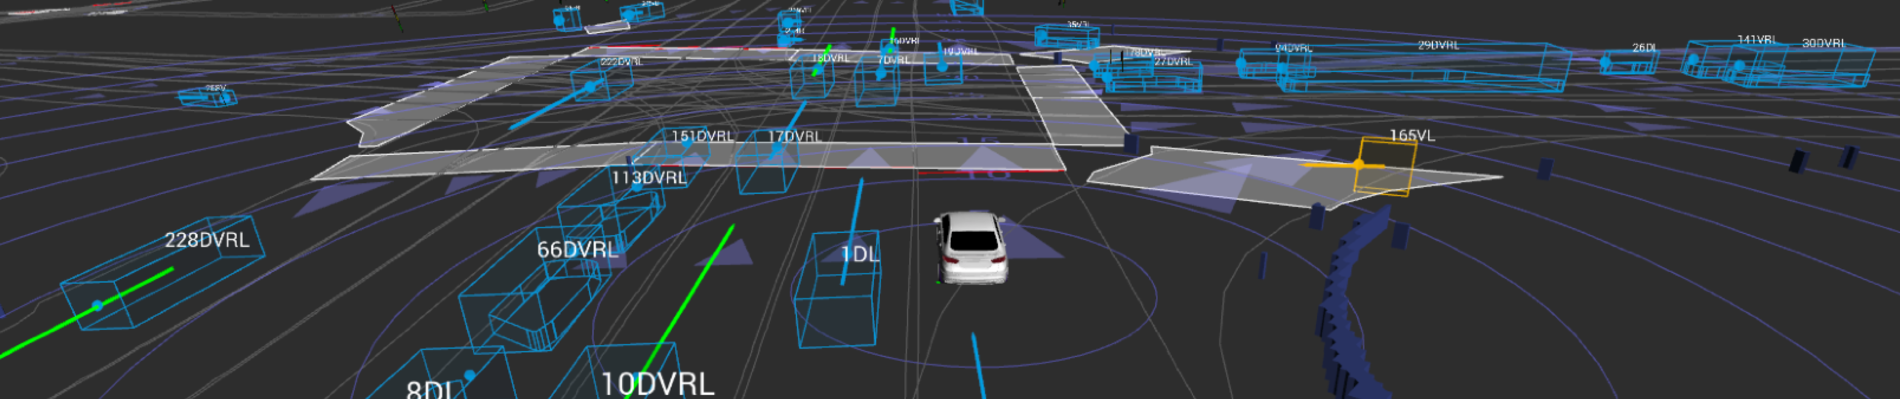
\includegraphics[width=0.9\textwidth]{images/lyft-hd-map.png}
  \caption{\textit{HD} мапа - \textit{Kaggle Lyft} \cite{kaggle_lyft} \label{kaggle-lyft-example}}
\end{figure}

На слици \ref{kaggle-lyft-example} се види пример визуализоване \textit{HD} мапе. Бело возило је агент, а плави правоугаоници су суседи. 
Са слике се види да мапе садрже и полигоне пешачких прелаза и још неке додатне податке. Подаци ових мапа су често у \textit{3D} формату
тј. узима се у обзир и висина. У реалном времену се ови подаци могу комбиновати са улазима из камера. 

\section{Циљ рада}

Циљ овог рада је анализа различитих приступа разумевања контекста сцена у саобраћају. 
Под контекстом се подразумева разумевање статичког дела сцене који обухвата путеве,
семафоре, пешачке прелазе и слично, динамичког дела сцене који обухвата историју кретања објеката на сцени, и интеракције 
свих елеманата у том окружењу. 

Сцене се посматрају из птичје перспективе
и дате су у формату \textit{HD} мапа. На основу информација добијених из обрађених мапа и историје трајекторије објеката
на сцени се врши предвиђање трајекторија агената. Посебна пажња се посвећује анализи већ постојећих
техника заснованих на растеризацији сцена и графовских техника које захтевају трансформацију података у структуру графа. 
Главна инспирација су хијеархијска графовска неуронска мрежа \textit{VectorNet} \cite{vectornet} и \textit{HOME} \cite{home}
архитектура која претежно заснована на примени конволутивних мрежа над растеризованим подацима. Поменути радови не нуде
имплементацију отвореног кода, као ни детаљне описе имплементације архитектуре.

Подаци једног сценарија (једна инстанца \textit{HD} мапе, један случај) нису нужно дати само у једном облику 
тј. само једној структури. Историја
трајекторија може да се чува у табеларном формату, где се за сваки ред чува временски тренутак, идентификатор агента и координате
тог агента у том тренутку. Мапа возног подручја може да буде задата као бинарна матрица где 1 означава да је могућа вожња на тој координати, 
а 0 да није могућа вожња. Први корак
сваке технике подразумева комбиновање и трансформацију података у одговарајући облик, било да је крајњи резултат слика или граф. У раду
се презентују детаљи имплементације припреме података у одговарајуће облике. 
Методе које се анализирају не нуде отворену имплементацију отвореног кода и не залазе у конкретне детаље имплементације. 

Квалитет модела зависи од начина на који се примењује доменско знање. Одређене кључне информације
са сцене могу да се изведу детерминистичким алгоритмима заснованим на одговарајућим хеуристикама. У раду се презентују
једноставне хеуристике које комбинују доменско знање са моделима машинског учења.

\section{Дефиниције појмова}

У овој секцији се дефинишу појмови који се користе у наствавку како би се олакшало разумевање самог рада:
\begin{itemize}
  \item Историја трајекторије - део трајекторије који је познат током процеса предвиђања.
  \item Реализација трајекторије - праве вредности трајекторије који нису познате током процеса предвиђања и користе се за упоређивање са предикцијом.
  \item Предвиђање трајекторије - крајњи резултат процеса предвиђања.
  \item Агент - Објекат који је у центру пажње током процеса предвиђања тј. објекат за који се врши предвиђање трајекторије. 
        Агент је углавном возило и не мора да буде јединствен на сцени.
  \item Крајња тачка трајекторије агента - Последња тачка реализације или предикције трајекторије агента.
  \item Сусед - Остали неагент објекти који се крећу на сцени. Осстали објекти су најчешће друга возила или пешаци.
  \item Путни сегмент - Део пута представљен као трајекторија.
\end{itemize}

\chapter{Преглед основних градивних елемената}
\label{chp:razrada}

\section{Неуронске мреже}

Дубоко учење је грана модерног машинског учења која се бави неуронским мрежама и учењем репрезентација. 
Ова грана машинског учења надмашује традиционалне методе када се ради са великом количином сирових података
као што су текст или слике. 
Неке од познатијих области примене су обрада сигнала, рачунарски вид и обрада природних језика. 
Главна разлика у односу на традиционалне методе је флексибилност у односу на структуру улазних података и
способност самосталног формирања својства. Ручно формирање својства за проблеме из области као што је рачунарски вид је за човека тежак
и временски захтеван задатак. Поред тога, углавном није могуће да се користе исте технике за издвајање својства за различите домене, него
процес издвајања својстава мора да се понавља.

\subsection{Потпуно повезане неуронске мреже}

Основни модел дубоког учења је потпуно повезана неуронска мрежа (\textit{eng. Fully connected Neural Network - FCN}) која
апроксимира произвољну непрекидну функцију. Мрежа се састоји из
низа слојева неурона. Вредност сваког неурона наредног слоја се рачуна као линеарна комбинација свих вредности неурона из претходног слоја. 
Сваки неурон из наредног слоја је на тај начин повезан са сваким неуроном из претходног слоја. Над израчунатим линеарним комбинацијама се примењује
активациона функција. Активациона функција неопходна ради апроксимације нелинеарних функција, јер композиција линеарних функција не може
да апроксимира нелинеарну функцију.  \cite{deep_learning_goodfellow, ml_mladen}.

Вредност функције $f$ која 
се апроксимира се добија \textit{пропагацијом унапред}, односно израчунавањем вредности сваког неурона редом почев од
\textcolor{red}{првог скривеног слоја до последњег}. На слици
\ref{ffn} је приказана потпуно повезана мрежа на апстрактном нивоу.
\textcolor{red}{У оквиру мреже се издвајају улазне вредности, скривени слојеви и излазни слој. На основу
вредности атрибута узорка из скупа података (улазне вредности) се апроксимира вредност функције $f$. Неурони излазног слоја имају апроксимиране вредности функције $f$, а
скривени међуслојеви су опциони и користе се у случају да сам излазни није довољан за апроксимацију функције $f$.
Улазне вредности се користе за израчунавање вредности првог скривеног слоја множењем вредности улаза тежинама. Када су израчунате вредности неурона првог скривеног слоја, онда се оне користе као улазне вредности за израчунавање
вредности у наредном слоју мреже \cite{deep_learning_goodfellow}.}

\begin{figure}[H]
  \centering
  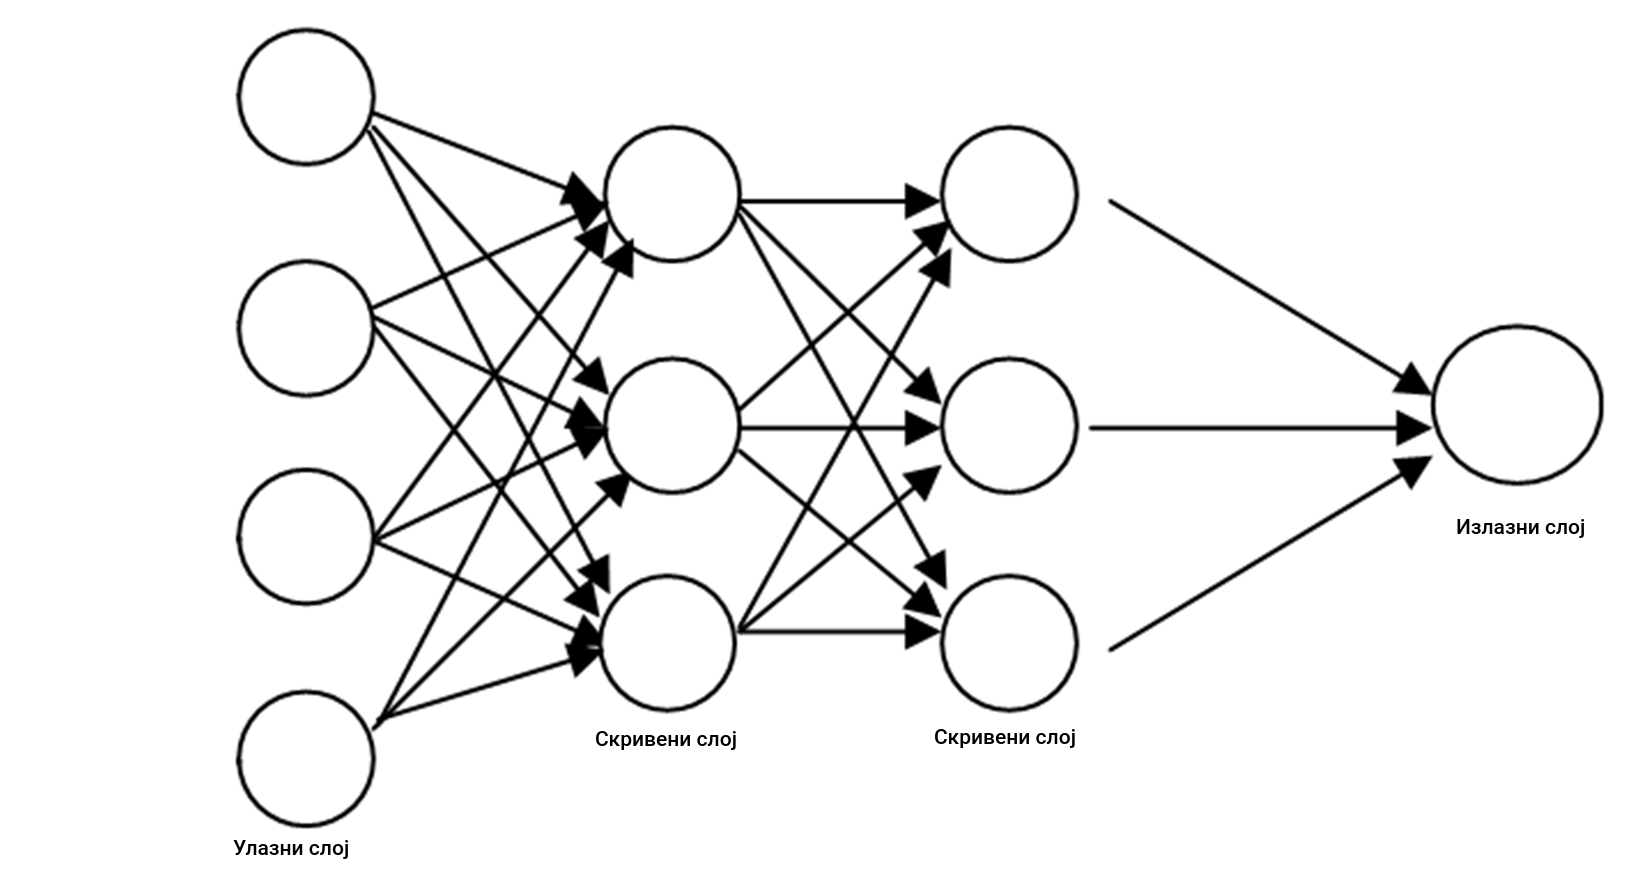
\includegraphics[width=0.9\textwidth]{images/ffn.png}
  \caption{Потпуно повезана мрежа \label{ffn}}
\end{figure}

Мрежа без скривених слојева тј. само са једним слојем тежине се назива перцептрон. Перцептрон може да апроксимира само линеарне функције и 
његове примене су ограничене. Да би мрежа могла да апроксимира било коју нелинеарну непрекидну функцију, неопходно је да има барем
један скривени слој са нелинеарном активационом функцијом. Мрежа са више скривених слојева без нелинеарне активационе функције
је еквивалентна перцептрону. Пример често коришћене
функције активације је \textit{ReLU (Rectified Linear Unit)}, где је $ReLU(x) = max(x, 0)$. 

Почетне вредности тежина слојева мреже се постављају да буду мале вредности из нормалне или униформне расподеле. Тренирање неуронске мреже
је оптимизациони проблем са циљем минимизације функције грешке $L$, где су тежине мреже параметри оптимизационог проблема. У случају регресије, 
функција грешке може да буде $L_2$ растојање између реализације и предикције, а у случају класификације то може да буде унакрсна ентропија.
За решавање овог оптимизационог проблема се користе методе
градијентне оптимизације под претпоставком да је функција $L$ диференцијабилна. 
Рачунање градијената се врши пропагацијом уназад \textit{(eng. backpropagation)}.

\subsection{Примена потпуно повезаних неуронских мрежа у раду}

У овом раду се потпуно повезане неуронске мреже користе за оцену кретања агента када је позната крајња тачка трајекторије агента. Проблем
оцене кретања није тежак када је крајња тачка позната и такав модел је једноставно тренирати. За обе архитектуре 
\textit{TNT-VectorNet} и \textit{HOME} се користи потпуно повезане мреже за оцену кретања агента.

\section{Конволутивне неуронске мреже}

Претходно поменуте потпуно повезане неуронске мреже имају велику моћ апроксимације, али не узимају у обзир топологију података. Постоје
различите архитектуре неуронских мрежа погодне за различите топологије података. Једна од најпознатијих архитектура су
конволутивне неуронске мреже (\textit{CNN - Convolutional Neural Network}) које се често успешно примеђују у процесирању сигнала (временских
серија) и процесирању слика. \cite{deep_learning_goodfellow}.

Сам назив архитектуре је добијен по операцији конволуције која као улаз узима два аргумента. Први аргумент је временска серија у случају
једнодимензионих сигнала или слика у случају дводимензионог сигнала, а други аргумент је филтер (кернел) којим
се издвајају својства из сигнала. Конволутивном применом
различитих филтера на сигнал се добија скуп својстава који могу да се користе у даљем процесу за класификацију или регресију. Традиционалне
методе подразумевају коришћење фиксних филтера за које је закључено да су прикладни за примену у датом домену проблема. Тренирањем модела
заснованих на конволутивним мрежама се уче аутоматски различити филтери. Након учења се очекује да се међу првим слојевима
уче једноставни облици као што су косе линије, док се на вишим нивоима разумеју компликованији облици као што је на пример око човека
\cite{deep_learning_goodfellow, ml_mladen}.

\subsection{Конволуција}

Под претпоставком да су дате функције $x$ и $w$, где се $x$ односи на сигнал, $w$ на филтер функцију и $t$ је временски параметар.
Тада се применом конволуције над $x$ и $w$ добија нови сигнал $s$:

\begin{figure}[H]
  \centering
  $s(t) = \int x(a)\cdot w(t - a) da = (x*t)(t)$
\end{figure}

Пример филтера $w$ је Гаусов филтер који упросечава сигнал и ублажава аутлајере. Подаци су увек коначни и дати у дискретном облику, 
па основни облик конволуција није применљив. Дискретна конволуција за сигнал дужине $n$ се дефинише као:

\begin{figure}[H]
  \centering
  $s(k) = \sum_{i=0}^{n-1} x(i)\cdot w(k-i)$
\end{figure}

У овом случају се $k$ односи на индекс узорка у низу вредности једнодимензионог сигнала. 
Операција се лако уопштава на примену на матрице уместо на низове. Нека је $X$ матрица на коју се примењује филтер $F$
(такође матрица), при чему се као резултат конволуције добија матрица $S$:

\begin{figure}[H]
  \centering
  $S(a, b) = (X*W)(a, b) = \sum_{i=0}^{n-1} \sum_{j=0}^{m-1} X(i, j) \cdot W(a-i, b-j)$
\end{figure}

На слици \ref{convolution} је приказан пример примене конволуције на \textit{2D} сигнал. У овом случају се као филтер користи
матрица димензије $2\times 2$ на слику (\textit{2D} сигнал) димензије $4\times 4$. Операција се своди на множење 
филтера са $2\times 2$ прозором слике који се помера по обе осе. Резултат се добија комбиновањем резултата
у једну матрицу димензије $3\times 3$ \cite{deep_learning_goodfellow}.

\begin{figure}[H]
  \centering
  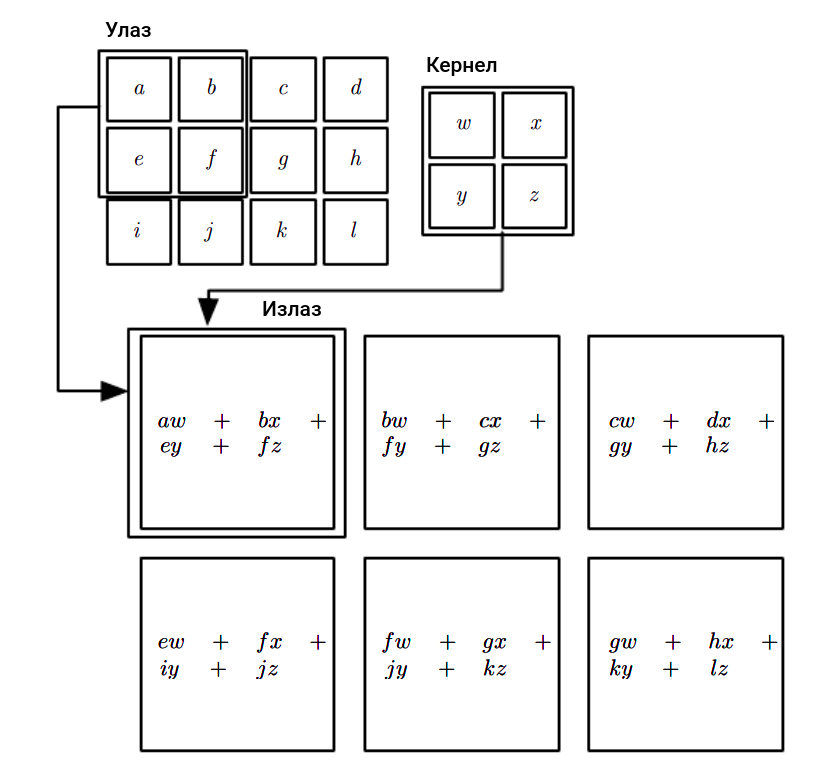
\includegraphics[width=0.6\textwidth]{images/convolution.png}
  \caption{Пример \textit{2D} конволуције\label{convolution}}
\end{figure}

У имплементацији конволутивних мрежа се уместо једног кернела (филтера) за сваки слој користи више њих и њихов број одговара броју излазних канала.
Мотивација са коришћење више филтера је могућност учења различитих облика са различитим филтерима.

\subsection{Агрегација}

Поред конволуција се често користи и агрегација (\textit{eng. pooling}). Агрегација је операција која мења сваки елемент матрице
статистиком која је израчуната на основу околине тог елемента матрице. Та околина је најчешће димензије $2\times 2$ или $3\times 3$ за слике,
а најчешће агрегације које се користе су максимум и просек. Циљ ове операције је смањивање величине улаза без значајног губитка 
информација. Агрегација има смисла само ако сигнали нису осетљиви на мање транслације, иначе постоји опасност губитка значајних информација. 
На слици \ref{maxpool} је приказан пример примене максимума димензије $3$ на једнодимензиони сигнал.

\begin{figure}[H]
  \centering
  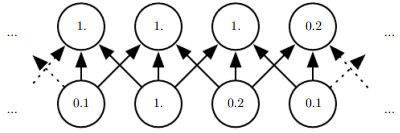
\includegraphics[width=0.5\textwidth]{images/maxpool.png}
  \caption{Пример агрегације\label{maxpool}}
\end{figure}

\subsection{Дубоке конволутивне неуронске мреже}

Конволутивне неуронске мреже су најчешће дубоке тј. састоје се из низа великог броја слојева неуронских мрежа. Типична конволутивна
мрежа садржи градивне елементе који се састоје редом од конволутивног слоја, нелинеарне активационе функције и агрегације. Дубока конволутивна
мрежа се састоји од низа оваквих елемената. У случају класификације слика се користи пар потпуно повезаних слојева испред коначног излаза из мреже.
На слици \ref{dcnn} је дат пример једне такве мреже \cite{deep_learning_goodfellow, ml_mladen}.

\begin{figure}[H]
  \centering
  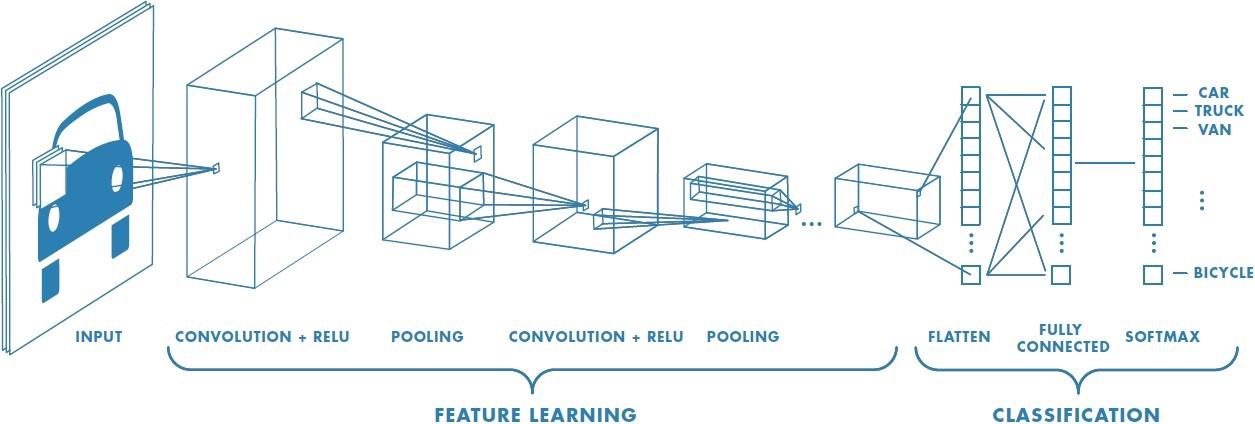
\includegraphics[width=1.0\textwidth]{images/dcnn.jpeg}
  \caption{Пример дубоке неуронске конволутивне мреже \label{dcnn}}
\end{figure}

\subsection{Транспоноване конволутивне неуронске мреже}

Комбинацијом конволутивних слојева и агрегација се улазна слика (дводимензиони сигнал) пресликава у векторску репрезентацију која има мању резолуцију, 
а већи број канала и садржи кључне информације за даљи процес предвиђања (погледати слику \ref{dcnn} - векторизован облик пре поравњања). 
У неким случајевима је потребно да излазна слика буде 
исте или сличне димензије као улазна слика. Примери где је то неопходно су пресликавање слика (\textit{eng. image translation}) тј. апроксимација
неке трансформације над сликама, одређивање маски детектованих објеката и отклањање шума са слике. Тада је неопходно да се
векторска репрезентација са мањом резолуцијом преслика у крајњи резултат. За те потребе се користе комплементарне операције у смислу
смањења и повећања резолуције слике. 

Комплементарна агрегацији је експанзија (\textit{eng. upsampling}) која само реплицира пикселе по свакој оси.
Пример експанзије је дат на слици \ref{upsampling}. 

\begin{figure}[H]
  \centering
  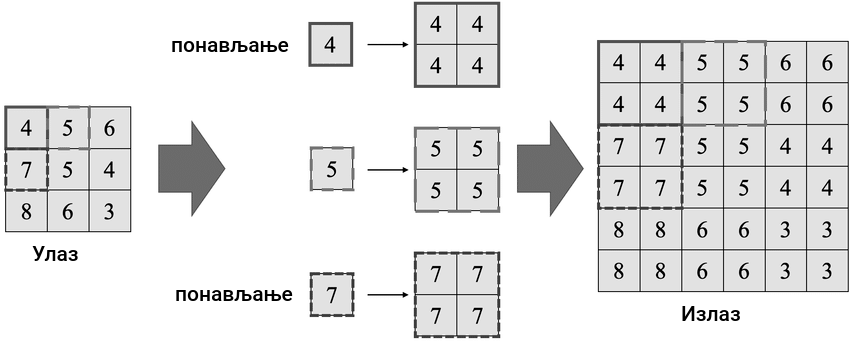
\includegraphics[width=1.0\textwidth]{images/upsampling.png}
  \caption{Пример експанзије \label{upsampling}}
\end{figure}

Комплементарна конволуцији је транспонована конволуција. Свако поље у улазној слици се множи кернелом транспоноване конволуције тако што
се сваки елемент кернела помножи вредношћу поља. Тада се за свако поље добија једна матрица димензије кернела и на основу њих се формира резултујућа
матрица тако да локација центра сваке матрице димензије кернела одговара пољу са којим је вршено множење. Уколико се неке матрице димензије кернела
поклапају у резултајућој матрици, онда се њихове вредности сабирају на пољима где се преклапају. Растојање између тих матрица димензије кернела
може да буде произвољно, а најчешће се узима вредност 2 како би резултајућа матрица била приближно 2 пута већа од улазне матрице.
На слици \ref{transpose-ccn} је дат пример транспоноване конволуције \cite{dive_into_deep_learning}.

\begin{figure}[H]
  \centering
  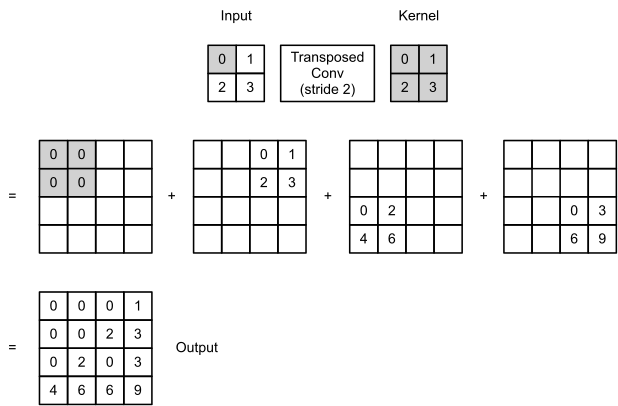
\includegraphics[width=1.0\textwidth]{images/transpose_cnn.png}
  \caption{Пример транспоноване конволуције \label{transpose-ccn}}
\end{figure}

\subsection{Примена конволутивних неуронских мрежа у раду}

Конволутивне неуронске мреже и транспоноване конволутивне неуронске мреже се користе за \textit{HOME} енкодер-декодер архитектуру за
генерисање топлотне мапе вероватноћа крајњих тачака трајекторије агента. За енкодер се користе класичне конволутивне мреже, а за
декодер се користе транспоноване конволутивне мреже \cite{home}.

\section{Графовске неуронске мреже}

Нека је $G = (V, E)$ усмерен граф, где је $V$ скуп чворова графа, а $E$ скуп грана графа. Свака грана је одређена
паром чворова, где је први елемент почетак гране, а други елемент је крај гране. Околина чвора $N(n), n \in V$ је скуп чворова из $V$ 
за које постоји излазна грана у чвор $n$. У наставку ове секције се користe претходнo дефинисани појмови са одговарајућим ознакама.

Графовске неуронске мреже (\textit{eng. Graph Neural Networks - GNN}) представљају скуп модела дубокох неуронских мрежа које могу да се примене на графовске структуре.
Главни изазов рада са графовским структурама је што стандардни алати као што су конволутивне неуронске мреже или рекурентне неуронске мреже
нису директно применљиви. Конволутивне мреже су погодне за податке структуиране као решетка, а рекурентне мреже су погодне за секвенце. За 
графовске структуре је неопходан мало другачији приступ \cite{grl}. 

Приликом кодирања чвора графа се поред својстава самог чвора узимају и својста околине. Пожељно је да мрежа која кодира та својста
буде инваријантна на пермутацију чворова тј. да њена функција не зависи од произвољног распореда колона и врста у матрици повезаности графа. Избор
операција које су инваријантне на распоред аргумената је мањи, што доноси додатне изазове при моделовању графовских неуронских мрежа \cite{grl}.

Основна особина које дефинише графовске мреже је \textit{размена порука између неурона (eng. neural message passing)}. Размена порука између неурона
подразумева кодирање и прослеђивање порука у облику вектора између суседа у графу и ажурирање својстава чворова на основу добијених порука. Размена
порука се врши кроз више итерација. Скривена репрезентација вектора чвора (\textit{eng. node hidden embedding}) $h^{(k)}_n$ се односи на 
векторску репрезентацију чвора $n \in V$ у $k$-тој итерацији размене порука. У нултој итерацији ($k=0$) сваки чвор има своја почетна својства. У 
свакој наредној итерацији се својства чвора ажурирају на следећи начин \cite{grl}:

\begin{figure}[H]
  \centering
  $h^{(k+1)}_n = \theta (h^{(k)}_n, \phi (\{h^{(k)}_v, \forall v \in N(v)\})) = \theta (h^{(k)}_n, m^{(k)}_{N_{n}})$
\end{figure}

Функција $\phi$ је произвољна диференцијабилна функција која агрегира скуп порука добијених из околине чвора $n$. Пошто је функција $\phi$
дефинисана над скупом, она је инваријантна на пермутацију чворова. Чести избори функције $\phi$ су сума, просек или максимум. 
Функција $\theta$ комбинује агрегиране поруке и репрезентацију вектора $n$ у
итерацији $k$ у нову векторизовану репрезентацију чвора $n$. У нултом кораку чвор $n$ има само информације о себи. У првој итерацији чвор $n$ има
информације о себи и свим чворовима у околини, а у другој итерацији додатно има информације о свим чворовима који су удаљени два корака од њега. 
Аналогно важи и за остале итерације. Уколико је број итерација велики, онда сваки чвор има информације о целом графу, али тиме сви чворови постају
слични. Због тога није идеално да графовске неуронске мреже у основном облику буду дубоке, што их разликује у односу на стандардне неуронске
мреже. На слици \ref{nmp} је приказан пример размене порука између неурона за дати пример графа за чвор $A$ \cite{grl}. 

\begin{figure}[H]
  \centering
  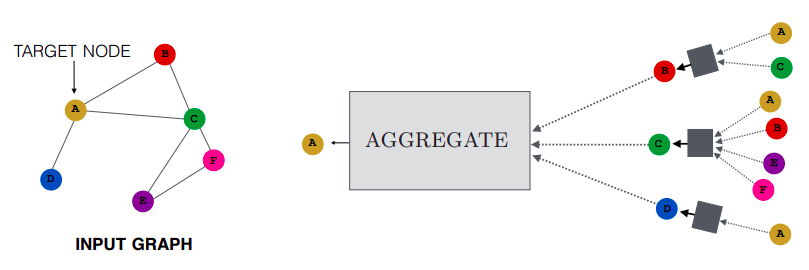
\includegraphics[width=0.7\textwidth]{images/nmp.png}
  \caption{Размена порука између неурона \label{nmp}}
\end{figure}

Нека је $A$ матрица повезаности и нека је $\theta (h^{(k)}_n, m^{(k)}_{N_{n}}) = \sigma (W^{(k)}_{self}\cdot h^{(k)}_n + W^{(k)}_{neigh}\cdot m^{(k)}_{N_{n}})$,
где је $\sigma$ активациона функција, а $W^{(k)}_{self}$ и $W^{(k)}_{neigh}$ су тежине за кодирање самог чвора и агрегираних порука суседа. Тада се у матричном облику
могу представити пресликавања својстава свих чворова:

\begin{figure}[H]
  \centering
  $H^{(k+1)} = \sigma (A\cdot H^{(k)}\cdot W^{(k)}_{self} + H^{(k)}\cdot W^{(k)}_{neigh})$
\end{figure}

Уобичајно је да се за сваки чвор додаје петља ка самом себи тј. постоји грана за сваки чвор $n$ која води у $n$. Тада матрица повезаности $A$
постаје $A+I$, где је $I$ јединична матрицa. У претходној формули $W_{self}$ и $W_{neigh}$ могу да се замене са $W$. На овај начин се 
ограничава могућност апроксимације мреже, али и смањује преприлагођавање модела. Претходна формула добија облик:

\begin{figure}[H]
  \centering
  $H^{(k+1)} = \sigma ((A+I)\cdot H^{(k)}\cdot W^{(k)})$
\end{figure}

Добијена формула има облик сличан графовским конволутивним мрежама које су описане у наставку.

\subsection{Графовске конволутивне мреже}

Графовске конволутивне мреже (\textit{eng. Graph Convolutional Network - GCN}) је једна од основних и најкоришћенијих архитектура графовских мрежа.
Главна разлика у односу на претходну формулу је у нормализацији матрице повезаности. Уколико се користи основни облик матрице повезаности,
онда је модел осетљив на степен чворова тј. чвор улазног степена 100 даје веће вредности након размене порука у односу на чвор улазног степена 1.
Ово отежава процес учења. Размена порука за графовске неуронске мреже се дефинише као \cite{grl}:

\begin{figure}[H]
  \centering
  $h^{(k+1)}_n = \sigma (W^{(k)}, \sum_{v \in N(n) \cup \{n\}} \frac{h_n}{\sqrt{|N(n)|\cdot |N(v)|}})$
\end{figure}

Пошто су степени сваког чвора $|N(n)|$ константе, онда нормализација може да се интегрише у матрицу повезаности тако да се добије
нормализована матрица повезаности $D$, па матрични облик постаје:

\begin{figure}[H]
  \centering
  $H^{(k+1)} = \sigma (D\cdot H^{(k)}\cdot W^{(k)})$
\end{figure}

\subsection{Примена графовских конволутивних мрежа у раду}

Графовске конволутивне мреже се користе за кодирање веза између сложених линија код \textit{VectorNet} \cite{vectornet} модела. Ове мреже
чине основу за подграф компоненту \textit{VectorNet} модела.

\section{Механизам пажње}

Механизам пажње имитира когнитивни процес у којем се човек селективно концентрише на делове неког контекста. У машинском учењу
се механизам пажње користи за препознавање битних елемената неког контекста. Функција механизма пажње може да се
представи као пресликавање упита $q$ и скупа парова кључева $K$ и вредности $V$ у излаз $o$. Све променљиве $q$, $K$, $V$ и $o$ имају
векторске репрезентације.
Променљиве $q$ и $o$ су матрице које имају само један ред, а $K$ и $V$ имају $d_v$ редова.
На апстрактном нивоу се кључеви $K$ упоређују са упитом $q$ и из сваког поређења се добијају тежине. Тамо где је упит ,,боље упарен`` са кључем,
већа је тежина за вредност која одговара том кључу. За одређивање тежина се користи скаларни производ. 
Тежине се нормализују \textit{softmax} функцијом тако да је њихов збир једнак 1.
Вредност вектора излаза $o$ је једнака тежинској суми свих вредности тј. редова из $V$. Више упита може паралелно да се израчунава ређањем
у матрицу $Q$ чиме се добија излаз $O$ тј. један ред за сваки упит:

\begin{figure}[H]
  \centering
  $O = Attention(Q, K, V) = softmax(Q\cdot K^T)\cdot V$
\end{figure}

Опционо може да се скаларни производ $Q\cdot K^T$ скалира вредношћу $\frac{1}{\sqrt{d_k}}$, где је $d_k$ број колона матрице $K$. Скалирање је погодно
у случајевима када је $d_k$ велики број. Претпоставка је да скаларни производ има огромну вредност за велико $k$. Последица великих вредности 
скаларног производа су мале вредности за градијент функције \textit{softmax} \cite{attention_is_all_you_need}. Формула у случају скалирања је следећа:

\begin{figure}[H]
  \centering
  $O = Attention(Q, K, V) = softmax(\frac{Q\cdot K^T}{\sqrt{d_k}})\cdot V$
\end{figure}

Матрице $Q$, $K$ и $V$ се добијају на основу улаза $X$ множењем са тежинама $W^{Q}$, $W^{K}$, $W^{V}$. тако да је $Q = X\cdot W^{Q}$, $K = X\cdot W^{K}$,
$V = X\cdot W^{V}$. Teжине $W^{Q}$, $W^{K}$, $W^{V}$ су параметри модела који се уче.

\subsection{Примена механизма пажње у раду}

У раду се механизам пажње користи у компоненти глобалног графа интеракције код \textit{VectorNet} модела. Циљ је да модел научи
са који елементима сцене агент интерагује и који елементи сцене су генерално релевантни за агента. 

\chapter{Преглед постојећих приступа}
\label{chp:razrada}
% ------------------------------------------------------------------------------

Уколико имамо више објеката на сцени за које треба да се изврши предвиђање трајекторија, онда је лакше да се предвиђање сваке 
трајекторије изврши из угла конкретног објекта. На тај објекат се у наставку реферише као на агента.
Сваки агент може да има свој референтни систем
и одговарајуће окружење у том систему тј. елементе сцене у околини тог агента. Скуп релеватних елемената као што су путеви, остала возила, пешаци и слично се
разликују од окружења једног агента до другог. Један од главних фактора за релеватност елемената је удаљеност тог елемента у окружењу од агента.

Предвиђање може да се извршава у једном кораку, где излаз модела подразумева више трајекторија (по једна трајекторија за сваког агента), 
или итеративно за сваког агента посебно. Сам приступ зависи од конкретног модела, 
али углавном су модели ограничени да итеративно генеришу предикције за сваког агента, што може да буде рачунски захтевније. 
Посматрано из угла аутономне вожње, скоро увек је интересантан само један агент на сцени који одговара возилу којим се управља.

Технике за предикцију трајекторија више објеката могу да се групишу грубо у четири групе:
\begin{itemize}
  \item Технике прилагођене репрезентацијама временских серија;
  \item Технике засноване на растеризацији;
  \item Технике засноване на графовским репрезентацијама;
  \item Хибридне технике.
\end{itemize}

У наставку ове главе биће укратко описане претходно наведене технике.

\section{Технике прилагођене репрезентацијама временских серија}

Из поставке проблема може да се закључи да овај проблем може да се сведе на предвиђање временских серија, јер свака 
трајекторија може да се представи помоћу временске серије. У том случају је интуитиван иницијални приступ да се користе рекурентне неуронске мреже
(\textit{eng. RNN - Recurrent Neural Network}) и конволутивне мреже за једнодимензионе сигнале (\textit{CNN - Convolutional Neural Network}). 
Често коришћена \textit{LSTM} архитектура рекурентних неуронских мрежа је погодна за кодирање динамике објеката на сцени. 
Динамика објеката се односи на историју трајекторија агента и осталих објеката на сцени.
У случајевима када трајекторија једног објекта зависи од трајекторија осталих објеката, није довољно да се само узима у обзир
историја трајекторије агента. У том случају је погодно да се користи механизам пажње као компонента модела која учи 
релевантне везе између различитих објеката на сцени \cite{argoverse, social_lstm, attention_is_all_you_need}. 

Један од главних проблема претходних приступа је неспособност модела да научи мултимодалну природу трајекторија на сцени. На слици
\ref{multimodal-example} је приказан пример сценарија где не постоји само једна валидна предикција трајекторије.
Ради успешног краткорочног планирања у аутономној вожњи, морају да се узму у обзир скоро сва могућа будућа стања сценарија. Модели
који као излаз дају само највероватнију трајекторију нису увек довољни. Бољи приступ је да се уместо модела који као излаз има највероватнију трајекторију користи
модел који као излаз има $N\ (N > 1)$ трајекторија заједно са вероватноћом сваке од тих трајекторија. Модели који се узимају у обзир у овом раду функционишу
по том принципу.

\begin{figure}[H]
  \centering
  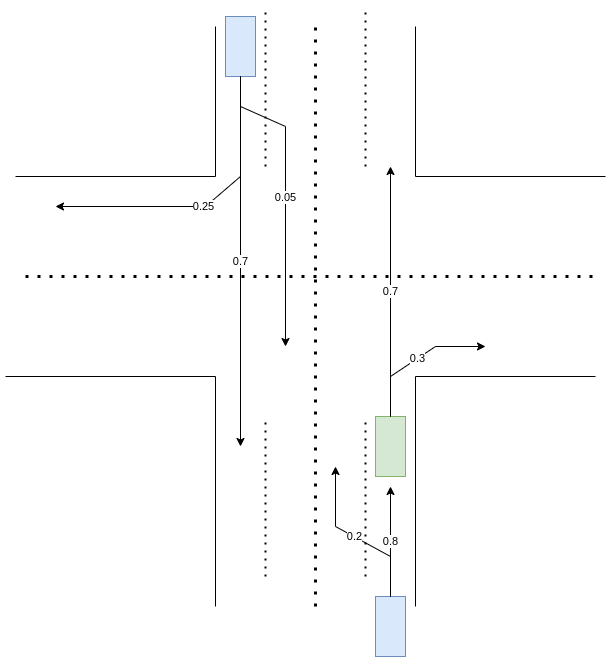
\includegraphics[width=0.5\textwidth]{images/multimodal.drawio.png}
  \caption{Милтимодална природа могућих будућих трајекторија - бројеви на трајекторијама представљају вероватноће}
  \label{multimodal-example}
\end{figure}

Битно је нагласити да трансформација модела који као излаз има једну трајекторију у модел који као излаз има више трајекторија није тако 
\textcolor{red}{једноставна.}
Природан избор за функцију грешке током тренирања је одступање предвиђене трајекторије од истините трајекторије. Конкретан пример
функције грешке је просечно еуклидско растојање тачака предвиђене трајекторије и истините трајекторије које одговарају истом временском тренутку. Ако
се тренира модел који предвиђа једну трајекторију са овом функцијом грешке (под претпоставком да квалитет и квантитет података нису проблем), 
онда ће он научити да предвиђа просечну трајекторију. Уколико се повећа број трајекторија у излазу модела, а функција грешке остане иста тј. предвиђене
трајекторије се упоређују са једном истинитом трајекторијм у сваком сценарију, то не значи да ће модел научити да узима у обзир и остале
вероватне трајекторије, већ ће вероватно генерисати само \textit{N} ,,дупликата`` трајекторија, где је \textit{N} број трајекторија у излазу 
тог модела. Овај проблем се назива колапс мода (\textit{eng. mode collapse}) и односи се на проблем игнорисања неких мода приликом генерисања предикција
\cite{overcoming_mode_collapse}.

Уместо учења модела који дају предикције трајекторија које су у просеку најбоље у тим случајевима, 
алтернатива је скуп модела заснованих на условним генеративним моделима који
омогућавају генерисање произвољног броја трајекторија кроз узорковање из условне расподеле 
(расподела је условљена историјом трајекторије, као и окружењем у којем се тај објекат налази). Овакви модели нису имуни на колапс мода,
али боље превазилазе тај изазов.
Пример таквог модела је \textit{Social GAN} \cite{social_gan} архитектура која узима у обзир претходно наведене услове и генерише ,,социјално прихватљиве`` 
трајекторије пешака. Током процеса предвиђања генеративни модели захтевају напредније алгоритме узорковања над великим бројем генерисаних
трајекторија ради оптимизације покривености трајекторијама тј. ради оптимизација 
односа будућих стања сценарија који је модел узео у обзир и свих могућих будућих стања сценарија. Чак и са одговарајућим алгоритмима,
није гарантована оптимална покривеност због стохастичког узорковања из латентног простора \cite{tnt}. Овакви модели могу да се користе
у аутономној вожњи, али су ипак погоднији за
проблем предвиђања трајекторија пешака у произвољном окружењу који није нужно улица, већ може на пример да буде и парк који има слабија ограничења
на кретање тог пешака.

\section{Технике засноване на растеризацији}

Растеризација подразумева трансформацију \textit{HD} мапа у слике, где слике приказују сцене из птичје 
перспективе (\textit{eng. BEV - Bird's-eye-view}). То значи да различите структуре података које описују један сценарио 
морају да се конвертују у облик слике. На пример, историја трајекторија која је углавном задата у табеларном формату мора да се конвертује 
у слику или да се на неки начин комбинује са растеризованим подацима у оквиру архитектуре модела.
Предност слика је могућност разумевања интеракција елемената на мапи 
коришћењем низа слојева конволутивних неуронских мрежа.
Идеја низа конволутивних мрежа је да преводу сирове слике у компактнији облик својстава који углавном има мању резолуцију, 
али већи број канала. Овако добијена својства се користе за предвиђање трајекторија.
Конволутивне мреже нису ограничене да раде са RGB и сличним форматима слика. Сваком пикселу може да се додели вектор својстава. 
Нека од очигледнијих својстава су: да ли агент заузима тај пиксел, да ли сусед (неагент) заузима тај пиксел,
да ли пиксел припада улици, ... Излаз CNN енкодера се углавном накнадно комбинује са осталим компонентама за генерисање резултата. 

Излази модела такође могу да се представљају као топлотне мапе \textit{(eng. heatmap)}. Структура топлотних мапа
одговара слици, где се сваком пикселу додељује вероватноћа
да се агент налази на тој локацији. За добијање топлотних мапа се користи енкодер-декодер архитектура, где се сирова слика
прво пресликава у компактнији облик својстава низом конволутивних слојева (енкодер), а онда се
применом низа транспонованих конволутивних слојева (декодер), које неформално представљају инверз конволутивних слојева, добија
топлотна мапа која је исте резолуције или редуковане резолуције у односу на улазну слику.
Како крајњи резултат треба да буде једна или више предикција трајекторија, неопходно је да се примени одговарајући алгоритам за
узорковање циљних тачака. Циљна тачка
се дефинише као последња локација предикције трајекторије. Главна мотивација за узорковање циљних тачака је претпоставка да уколико је познато где се
трајекторија завршава, онда је лако да се одреди цела та трајекторија тј. оцени кретање агента до крајње
тачке.\footnote{Претпоствка важи
у случају када је агент возило које у саобраћају има ограничено кретање, док у случају човека који се креће у неком парку то није толико реална
претпоставка.} Број узоркованих крајњих тачака зависи од алгоритма и може да буде фиксан или да варира од једног до другог сценарија. 
Пример алгоритма је узорковање N циљних тачака тако да површина које њихове околине покривају има највећу сумарну вредност вероватноћа 
пиксела топлотне мапе. Околина
тачке може да буде круг са фиксном величином полупречника који представља параметар алгоритма узорковања. Када је позната циљна тачка трајекторије,
онда може да се користи једноставнији модели неуронских мрежа (нпр. потпуно повезане мреже) \cite{home, centernet}.

Архитектура \textit{HOME} \cite{home} користи принцип за паралелно кодирање растеризоване сцене (статички део)
и трајекторија oбјеката (динамички део). Резултати
статичког и динамичког дела модела се спајају конкатенацијом и прослеђују као улаз у декодер за генерисање топлотне мапе. 
Узорковањем тачака из топлотних мапа се добија скуп циљних тачака. Различити алгоритми узорковања дају
боље перформансе модела по различитим метрикама за евалуацију квалитета трајекторија у аутономној вожњи. Независно од модела топлотне мапе
се тренира модел који оцењује кретање трајекторије када је позната њена крајња тачка.

Могуће је растеризовати потпуно податке тј. растеризовати и трајекторије као низ слика. Свака слика садржи скуп тачака које представљају
локације објеката. Архитектура \textit{CASPNet} \cite{caspnet} примењује CNN енкодер на свако стање историје сценарија 
и користи ConvLSTM \cite{convlstm} модел за разумевање
темпоралних веза тих слика. На овај начин се добијају својства динамичког дела сцена. 
На сличан начин је могуће и извући својства и за 
статички део (возне линије, возни површине, ...) користећи класичне конволутивне мреже. Комбинацијом ових података се генеришу
трајекторије које су исто дате у растеризованом облику. Овакав приступ је рачунски веома скуп.

\section{Технике засноване на графовским репрезентацијама}

Мапе имају комплексну топологију, а технике засноване на растеризацији користе конволуцију која тешко 
извлачи потпуно семантику тих мапа. Taкође, конволуција је скупа операција. Алтернатива је моделовање мапа графовским структурама. 
Технике засноване на графовском репрезентацијом као улаз добијају стање мапе кодиране као граф и примењују моделе графовских неуронских мрежа. 
Две архитектуре које представљају основе за већину архитектура ове групе су \textit{LaneGCN} \cite{lanegcn} и \textit{VectorNet} \cite{vectornet}.

Мапа може да се моделује као скуп повезаних сложених линија (\textit{eng. polylines}), где сваком објекту одговара једна усмерена сложена линија. 
\textit{VectorNet} је хијерархијска графовска неуронска мрежа која као улаз добија мапу која је моделована као скуп 
сложених линија, а као резултат даје предикцију једне трајекторије за сваког агента.\footnote{У овом контексту се издвајају агенти
као објекти на сцени за које се врши предвиђање трајекторије.} Идеја је да се прво извуку својста из сложених 
линија појединачних објеката, а онда пронађу одговарајуће међусобне везе између објеката и везе између објеката и возних линија. 
За проналазак међусобних веза се користи механизам пажње \cite{attention_is_all_you_need, vectornet}.
Мотивација је следећа: Нису сви објекти у околини значајни за конкретног агента,
јер они објекти који су далеко од њега и иду супротном линијом не утичу толико на његово кретање. Нису ни сви путни сегменти значајни за агента.
Свакако су значајни путни сегменти који се поклапају са историјом трајекторије агента и путни сегменти по којим агент може потенцијално да се креће
у скоријој будућности. Задатак модела је да закључи који елементи сцене су значајни.

Архитектура \textit{LaneGCN} нуди варијанту конволутивних графовских мрежа (\textit{GCN - Graph Convolution Network}) \cite{gcn}
која је специјализована за графове путних сегмената које имају различите типове веза. Користе се различите матрице
повезаности за суседе, претходнике, следбенике (леви и десни) у контексту путних сегмената. 
За сваку матрицу повезаности може да се примени класичан GCN, а
комбиновањем тих елемената је добија један \textit{LaneGCN} слој \cite{lanegcn}. Сам модел се своди на \textit{GCN} са више матрица повезаности.

\section{Хибридне технике}

Хибридне технике користе комбинацију структура графова и BEV слика. Модел \textit{GOHOME} је модификована верзија \textit{HOME} 
модела који уместо CNN енкодера и растеризоване слике као улазне податке, користи \textit{LaneGCN} архитектуру као енкодер и податке
у облику графа. Заправо ансамбл ова два модела \textit{HOME} и \textit{GOHOME}
даје најбоље резултате по \textit{MR} метрици.\footnote{Објашњење за ову метрике се налази у секцији о евалуацији.}

\section{Технике засноване на облацима тачака}

Последња група нешто одступа од осталих по броју објављених радова, 
али и даље даје добре резултате. Подаци се посматрају као облаци тачака (\textit{eng. point cloud}) 
и примењују се технике намењене за такву структуру података. Основна
архитектура је \textit{TPCN} \cite{tpcn} која је заснована на \textit{PointNet} \cite{pointnet}. Већина осталих техника су ,,изведене`` из ње.

% ------------------------------------------------------------------------------
% ------------------------------------------------------------------------------

\chapter{Метрике за евалуацију модела}
\label{chp:razrada}
% ------------------------------------------------------------------------------

Неке од стандардних метрика за евалуацију квалитета предикције трајекторија су ,,просечнa грешка одступања`` (\textit{eng. ADE - Average Displacement Error})
и ,,грешка последњег одступања`` (\textit{eng. FDE - Final Displacement Error}). У наставку се користе енглеске скраћенице \textit{ADE} и
\textit{FDE}. Метрика \textit{ADE} се рачуна као просечно еуклидско растојање између тачака предикције и истините трајекторије у свим
временским тренуцима који одговарају тој трајекторији. 
Метрика \textit{FDE} узима у обзир само последњу тачку тј. еуклидско растојање између последње тачке реализације и предикције.
Што су метрике \textit{ADE} и \textit{FDE} мање након евалуације модела, то је модел квалитетнији. \cite{social_gan, argoverse}.  
У наставку се налазе формуле у случају да се посматра тачно један објекат (нпр. само агент):

\begin{figure}[H]
  \centering
  $ADE = \frac{1}{T}\sum_{k=1}^{T}\sqrt{(x_k - \hat{x}_k)^2 + (y_k - \hat{y}_k)^2}$
\end{figure}


\begin{figure}[H]
  \centering
  $FDE = \sqrt{(x_{T} - \hat{x}_{T})^2 + (y_{T} - \hat{y}_{T})^2}$
\end{figure}

У наведеним формулама $T$ означава дужину трајекторије агента која је добијена узорковањем локација објекта у дискретним тренуцима, 
$(x_{1}, y_{1}), (x_{2}, y_{2}), ..., (x_{T}, x_{T})$ су $T$ узастопних локација агента на изабраном интервалу. 
Метрике се једноставно уопштавају у случајевима где постоји N објеката на сцени:

\begin{figure}[H]
  \centering
  $ADE = \frac{1}{T\times N}\sum_{n=1}^{N}\sum_{k=1}^{T}\sqrt{(x^{(n)}_k - \hat{x}^{(n)}_k)^2 + (y^{(n)}_k - \hat{y}^{(n)}_k)^2}$
\end{figure}

\begin{figure}[H]
  \centering
  $FDE = \frac{1}{N}\sum_{n=1}^{N}\sqrt{(x^{(n)}_{T} - \hat{x}^{(n)}_{T})^2 + (y^{(n)}_{T} - \hat{y}^{(n)}_{T})^2}$
\end{figure}

Ако узмемо у обзир претпоставку да се релативно детерминистички може одредити трајекторија ако је дата њена последња тачка 
(што је у случају возила у сабраћају разумна претпоставка), онда су ове две метрике корелисане у смислу да модел 
који има добар \textit{FDE}, има и добар \textit{ADE} (и супротно).

Ове једноставне метрике су погодне под претпоставком да је расподела трајекторија унимодална у односу на дату историју тј. да за сваку историју трајекторије 
постоји тачно једна смислена предикција. 
Скупови података трајекторија могу да имају јачу стохастичку природу због природе самог проблема или због непотпуних информација о окружењу.
Пример таквог скупа података је скуп трајекторија пешака. Пешак који је прешао пешачки прелаз, може у том тренутку да скрене лево или десно.
У том случају имају два вероватна сценарија за исту историју трајекторије, али углавном немамо информације о циљевима самог пешака \cite{social_gan, best_of_many_cvae}. 
У случају возила је ситуација мало блажа због већег броја ограничења која за последицу имају да су трајекторије возила
лакше за предвиђање од трајекторија пешака. На слици \ref{multimodal-example} је већ приказан пример једног сценарија у саобраћају где
се за исту историју могу очекивати различити исходи.

Скуп метрика ,,најбољи из групе`` (\textit{eng. ,,Best of Many``}) узимају у обзир мултимодалну природу расподела трајекторија. Модел може
да генерише неколико различитих предикција трајекторија и да за сваку предикцију да одговарајућу вероватноћу (поузданост). 
За рачунање грешке се узима предикција која је најбоља по дефинисаном критеријуму. Критеријум не мора да се поклапа са самом мером која се користи 
тј. не мора нужно да се изабере трајекторија која је најбоља по тој мери, већ за тај избор може да се користи друга мера. 
Конкретан пример такве метрике је \textit{minADE} која ће бити описана у наставку \cite{best_of_many_cvae, argoverse}. 
Претходно наведене метрике \textit{ADE} и \textit{FDE} се уопштавају у \textit{minADE} и \textit{minFDE}. Због једноставности узимају се у обзир облици
са једним објектом: \cite{Disdis, best_of_many_cvae}

\begin{figure}[H]
  \centering
  $minADE = ADE(\displaystyle\argmin_{k \in \{1, ..., K\}} FDE(\hat{A}_k, A), A)$
\end{figure}

\begin{figure}[H]
  \centering
  $minFDE = \displaystyle\min_{k \in \{1, ..., K\}} FDE(\hat{A}_k, A)$
\end{figure}

Овде је $A_k = ((x^{(k)}_1, y^{(k)}_1), (x^{(k)}_2, y^{(k)}_2), ...,  (x^{(k)}_T, y^{(k)}_T))$ истинита трајекторија, а 
$\hat{A}_k = ((\hat{x}^{(k)}_1, \hat{y}^{(k)}_1), (\hat{x}^{(k)}_2, \hat{y}^{(k)}_2), ...,  (\hat{x}^{(k)}_T, \hat{y}^{(k)}_T))$ 
трајекторија из скупа предикција. Обе метрике \textit{minFDE} и \textit{minADE} 
се своде на избор трајекторије која најмање одступа од истините трајекторије у последњем тренутку тј. бира се трајекторија која има најмањи \textit{FDE}.

Уколико модел генерише више од \textit{K} трајекторија, узима се и обзир првих \textit{K} по поузданости. У специјалном случају када је $K = 1$, онда 
\textit{minFDE} постаје \textit{FDE}, a \textit{minADE} постаје \textit{ADE}. 
Проблем са \textit{minADE} i \textit{minFDE} је у томе што не узимају у обзир остале трајекторије поред најбоље и самим тим се не прави разлика
између предикције са свим добрим трајекторијама и предикције са једном добром трајекторијом \cite{Disdis}. 
Друга замерка овим метрикама је што не узимају у обзир поузданост предикција након филтрирања \textit{K} трајекторија. Уколико је најбоља трајекторија
прецизна, желимо и даље да знамо да ли је модел сигуран или је добар резултат последица ,,среће``. Модификоване метрике \cite{home}: 

\begin{figure}[H]
  \centering
  $p\mbox{--}minADE = ADE(\hat{A}_{min}, A) - \ln{P(\hat{A}_{min}|E)}$
\end{figure}

\begin{figure}[H]
  \centering
  $p\mbox{--}minFDE_{prob} = FDE(\hat{A}_{min}, A) - \ln{P(\hat{A}_{min}|E)}$
\end{figure}

Овде је $\hat{A}_{min}$ трајекторија која има најбољу $FDE$ оцену, а $P(\hat{A}_{min}|E)$ је условна вероватноћа те 
трајекторије $\hat{A}_{min}$ у односу на стање окружења $E$. Уколико је мала грешка по метрици \textit{ADE} (\textit{FDE}) за одговарајућу трајекторију, 
али њена вероватноћа има малу вредност, онда негативан логаритам те вероватноће има велику вредност \cite{argoverse}.
У импементацији се ова вероватноћа ограничава са доње стране, како не
би дошло до прекорачења због велике апсолутне вредности након примене логаритма на веома мале вредности.

Одступање крајње тачке које је 1 или 2 метра даље од реализације није толико релевантно у односу на одступање од 
неколико метара \cite{home}. Метрика $MR^{\alpha}_{K}$ (\textit{eng. Miss Rate - "проценат промашаја"}) даје информацију
колико су процентуално чести случајеви великих одступања тј. ситуација у којима је промашена мода. Ова метрика се дефинише на следећи начин: 
нека је дат мултимодални скуп података димензије $N$ и нека се за сваки елемент из скупа података генерише $k$ предикција (трајекторија). Ако
у $M$ случајева крајња тачка најбоље од тих $K$ трајекторија одступа за више од $\alpha$ од истините крајње тачке, 
онда је $MR^{\alpha}_{K} = \frac{M}{N}$. Најбоља трајекторија од $K$ предвиђених је она која је најбоља по \textit{FDE} метрици тј.
крајња тачка те трајекторије је најближа крајњој истинитој тачки. За параметар $\alpha$ се узима вредност $2m$ за \textit{Argoverse} 
скуп података \cite{argoverse}. Дефиниција метрике се компактно записује на следећи начин:

\begin{figure}[H]
  \centering
  $MR^{\alpha}_{k} = \frac{1}{N}\cdot \sum^N_{n=1} I(\displaystyle\min_{k\ \in\ \{1..K\}}||\hat{A}^{k}_{n} - A_{n}||_{2} > \alpha)$
\end{figure}

Такође постоји верзија метрике која узима у обзир вероватноћу и кажњава предикцију модела ако је добра, а модел је ипак несигуран. \cite{argoverse}
Обична $MR^{\alpha}_{k}$ метрика рачуна само број тачака трајекторије које одступају много од одговарајуће тачке истините трајекторије, док
$MR^{\alpha}_{k}{prob}$ додатно кажњава ситуације у којима не постоји велико одступање, али модел није довољно сигуран. 

Све до сада наведене метрике имају примену и ван аутономне вожње. Пошто је агент углавном возило, може да
се анализира да ли предвиђена трајекторија скреће са пута. Због тога се уводи метрика ,,сагланост са возним подручјем`` 
(\textit{eng. DAC - Drivable Area Compilance}), која одређује учесталост трајекторија које нису скренуле са пута од изабраних 
\textit{K} трајекторија \cite{argoverse}:

\begin{figure}[H]
  \centering
  $DAC = \frac{DAC_{occ}}{T}$
\end{figure}

У претходној формули се $DAC_{occ}$ односи на број трајекторија које су скренуле са пута од Т предвиђених трајекторија. 
У евалуацији модела се узимају у обзир све метрике. За параметар \textit{K} за \textit{minADE} и \textit{minFDE} се узима вредност 6,
као што је то урађено у већини радова на ову тему.

\chapter{Припрема података \label{initprep}}

Основни скуп података за тренирање и тестирање техника предвиђања трајекторија је \textit{Argoverse Motion Forecasting} скуп података
који се састоји од 324 хиљаде сценарија у саобраћају сачиуваних као \textit{HD} мапе. Постоје две групе \textit{HD} мапа
за градове Питсбург и Мајами. Коришћењем аутономних возила су генерисани сценарији који представљају неколико узастопних слика сцена (у табеларном формату)
на деловима мапа. Сви детаљи о овом скупу података се могу пронаћи на адреси 
\href{https://www.argoverse.org/index.html}{\color{blue}{www.argoverse.org}} \cite{argoverse}. \\


\noindent Kључне информације које се издвајају из сваког сценарију су:
\begin{itemize}
  \item Мапа сценарија (Питсбург или Мајами);
  \item Трајекторије агената;
  \item Трајекторије осталих објеката на сцени (суседи);
  \item Путни сегменти.
\end{itemize}

У наставку се описује процес прве фазе припреме података. Формат података који се добија након ове фазе је погодан
за даљу трансформацију у графовску структуру или слику (растеризован облик).

У табели \ref{dp-params-table} се види преглед свих параметара процеса који ће
бити детаљно објашњени у наставку ове главе. Параметри $N_r$ и $N_h$ су изабрани тако да се поклапају
са осталим радовима. Ако би ти параметри били другачији, онда поређење метрика нема толико смисла. 
Престпоставка је да претрагом осталих параметара може да се повећа квалитет података за учење, а самим тим
и квалитет модела. Како је та опција рачунски јако скупа, у овом случају се прескаче.

\begin{table}[H]
  \centering
  \begin{tabular}{c|c}
    Ознака параметра & Објашњење \\
    \hline
    $N_r$ & Дужина трајекторије реализације \\
    \hline
    $N_h$ & Дужина трајекторија историје \\
    \hline
    $N_{hmin}$ & Минимална дужина историје трајекторије агента \\
    & пре допуњавања \\
    \hline
    $N_{homin}$ & Минимална дужина историје трајекторије суседа \\
    & пре допуњавања \\
    \hline
    $N_{romin}$ & Минимална дужина трајекторије реализације суседа \\
    & пре допуњавања \\
    \hline
    $T_{steps}$ & Умножак максималног растојања до сегмента пута \\
    \hline
    $D_{lsinit}$ & Минимални радијус за проналазак путних сегмената \\
    & у околини посматраног агента \\
    \hline
    $D_{lsmax}$ & Максимално растојање до пута \\
    \hline
    $K_{ls}$ & Корак умножак радијуса за проналазак путних сегмената \\
    \hline
    $K_c$ & Број најбољих путних сегмената по \textit{DTW} методи \\
    \hline
    $\theta_{min}$ & Најмањи угао између правца путног сегмента \\
    & и правца трајекторије агента
  \end{tabular}
  \caption{Преглед параметара припреме података}
  \label{dp-params-table}
\end{table}

\section{\textit{Argoverse} интерфејс}

Сирови подаци сваког сценарија се векторизују и чувају у полу-структуираном формату. 
За парсирање и обраду улазних података се користи \textit{argoverse API} интерфејс. Сваки град се састоји из скупа
повезаних путних сегмената који чине један усмерен граф. Функције које се користе из \textit{Argoverse} интерфејса се 
односе на операције над тим графом. Скуп функција које се користе:
\begin{itemize}
  \item Одређивање свих путних сегмената који се налазе у околини агента на основу последње тачке у историји трајекторије.
  \item Одређивање следбеника, претходника и суседа у графу у односу на посматрани путни сегмент.
  \item Читање метаподатака о путним сегментима: Да ли се путни сегмент налази у неком пресеку, да ли постоји контрола саобраћаја и
        да ли је путни сегмент усмерен лево, десно или је прав.
  \item Примена претраге у дубину над графом у односу на посматрани путни сегмент који представља почетни чвор у алгоритму претраге.
  \item Одређивање путног подручја града (матрица).
\end{itemize}

Циљ овог корака процесирања података је векторизација података у формат који је је независан од модела који се користи тј.
обједињавање заједничког дела припреме података.

\section{Припрема трајекторије агента}

Трајекторија агента\footnote{Низ $(x, y)$ тачака, где је приближна временска разлика између две тачке око 0.1 секунди у \textit{Argoverse}
скупу података.} 
се дели на два дела: историја (својства) и реализација (будуће вредности). Реализација се састоји од $N_r$ вредности
$x$ и $y$ координата тј. векторизована димензија је $N_r\times 2$.
Историја се аналогно формира да садржи историју $N_h$ опажања $x$ и $y$ координата. Овај део трајекторије иде непосредно
пре реализације. То значи да је за један елемент скупа података неопходно $N_h + N_r$ тачака у једном сценарију. 
Сценарио се дефинише као део мапе града који се посматра
у одређеном временском интервалу. Скуп података није већ
дат у том формату и може да има произвољан број координата агента у једном неприпремљеном сценарију. Посматрају се следећи случајеви:
\begin{itemize}
  \item Постоји више од $N_h + N_r$ опажања: Одбацује се реп трајекторије (првих неколико вредности хронолошки гледано).
        Уколико је скуп података мали (што не важи за \textit{Argoverse} скуп података), може се узорковати више временских интервала
        опажања и да се за сваки формира по један сценарио.
  \item Постоји мање од $N_{hmin} + N_r$ опажања, где је $N_{hmin}$ минимална дужина историје трајекторије: Сценарио се одбацује (сматра се да је невалидан).
  \item Постоји између $N_{hmin} + N_r$ и $N_h + N_r$ опажања: реп трајекторије који се односи на историју трајекторије 
        се допуњава до димензије $N_h + N_r$ посматрано као да објекат мирује у тим тренуцима.
\end{itemize}
Уколико је историја
трајекторије скоро потпуно непозната, онда није реално да се очекују добре перформансе модела на том сценарију. Филтрирање се
односи на скуп података за учење, а током предвиђања је свакако неопходно да се да неки резултат. Параметар $N_r$ је постављен на \textit{30},
а $N_h$ је постављен на \textit{20}. Ове вредности су изабране тако ради усаглашавања са осталим радовима. Параметар $N_{hmin}$ је
постављен на \textit{5}, али избор вредности је флексибилан. 
Коначно, облик историје је $(N_h, 3)$, где трећа вредност означава да ли је опажање право ($1$) или допуњено ($0$).

Све координате се нормализују тако да су релативне у односу на последње опажање историје агента. Последње опажање историје
агента има координату (0, 0) у новом координатном систему, а све остале тачке се транслирају за вектор $-C$, где је $C$ оригинална позиција
последњег опажања. Координатни систем се такође ротира тако да се вектор који је одређен првом и последњом тачком историје трајекторије,
што чини наивно апроксимиран правац трајекторије, поклапа са \textit{y}-осом сличко као и у оригиналном \textit{Vectornet} раду \cite{vectornet}. Последња
трансформација је скалирање свих координата са $\frac{1}{25}$, где је ова вредност добијена анализом стандардних девијација свих тачака
на сценаријима (узета је просечна вредност свих сценарија). Ове трансформације су кључне за перформансе модела, јер је сам проблем који се решава
једноставнији:
\begin{itemize}
  \item Применом транслације модел не мора да учи где се агент налази, јер је то увек (0, 0) координата;
  \item Применом ротације моделу је олакшано учење усмерења трајекторије тј. моделу је лакше да одреди оријентацију агента;
  \item Применом скалирања се добијају стабилнији градијенти.
\end{itemize}
Оригинална позиција последњег опажања и угао ротирања се чувају за сваки сценарио. На овај начин је могуће извршити
инверзно пресликавање у оригинални координатни систем. За све метрике наведене у претходој секцији сем \textit{DAC} је довољно
да се само изврши инверзно скалирање, јер су транслација и ротација изометрије које чувају растојања. За метрику \textit{DAC} је 
неопходно да се изврши усклађивање са мапом путног подручја.

\section{Припрема трајекторија суседа}

Трајекторије суседних објеката се деле на два дела аналогно трајекторији агента. Неопходно је да се синхронизују трајекторије 
суседних објеката по временским ознакама (eng. \textit{timestamp}) са трајекторијом агента, јер не постоји у сваком тренутку исти
број објеката на сцени. Након синхронизације се трајекторије деле на историју и реализацију и проверава се да ли дужине тих
делова задовољавају критеријуме:
\begin{itemize}
  \item Уколико је дужина трајекторије историје краћа од $N_{homin}$, где је $N_{homin}$ минимална дужина историје трајекторије суседа: 
        Објекат се одбацује;
  \item Уколико је дужина трајекторије реализације краћа од $N_{romin}$, где је $N_{рomin}$ минимална дужина реализације трајекторије суседа, Објекат исто одбацује.
\end{itemize}
Вредности параметара $N_{homin}$ и $N_{romin}$ се постављају на \textit{5} и \textit{3}.

Као додатна провера, за сваког суседа се провера растојање од агента. Уколико је сусед превише далеко, онда се се он одбацује.
Критеријум за одбацивање суседа узима у обзир брзину агента (по $x$ и $y$ оси одвојено) и растојање њихових последњих опажања
у трајекторији историје. Уколико неки од следећих услова није
испуњен, онда се сусед игнорише у сценарију: 
\begin{itemize}
  \item $\frac{O_n^x}{V_s^x} \leq T_{steps}$
  \item $\frac{O_n^y}{V_s^y} \leq T_{steps}$
\end{itemize}
где је $O_n^x$ ($O_n^y$) нормализована $x$ ($y$) координата суседа $n$, $V_s^x$ ($V_s^y$) је наивно
апроксимирана брзина агента $s$
по $x$ ($y$) оси\footnote{Брзина се апроксимира као просек промена координата у трајекторији историје.} и $T_{steps}$ је параметар толеранције.
Трајекторије се секу или допуњавају до фиксног облика (kao што је то у случају припреме трајекторије агента). 
Фиксна димензија сваке трајекторија суседа омогућава да се историје трајекторија свих изабраних суседа представе у компактно векторизованом
облику димензије $N_n\times N_h\times 3$. Аналогно важи и за реализацију трајекторија свих изабраних суседа које могу да се представе у векторизованом
облику димензије $N_r\times N_h\times 3$. Прве две вредности треће димензије се односе на $x$ и $y$ координату, а 
трећа вредност је информација о томе да ли је та тачка допуњена или не.

\section{Припрема путних сегмената}

Скуп података Argoverse садржи информацијфе о путевима сваког града структуиране као скуп краћих путних сегмената
којима су додељени атрибути који их додатно описују и који ће бити описани у наставку. Како за конкретан сценарио нису битни сви путни сегменти
графа, већ само они који се налазе у околини агента, неопходно је да се изврши филтрирање путних сегмената. Овај део припреме се ослања на 
\textit{argoverse-api} пакет.

Путни сегменти се такође приказују као трајекторије. За координате путног сегмента се узима централна линија путног сегмента
која чини скуп тачака на средини пута у односу на ширину.

На основу локације агента се издвајају путни сегменти који су у околини агента са радијусом $D_{lsinit}$ по $L_1$ растојању. 
Уколико нема пронађених сегмената централних линија, онда се вредност за $D_{lsinit}$ множи са $K_{ls}$\footnote{$D_{lsinit}$ и $K_{ls}$ су фиксне вредности
у \textit{argoverse} интерфејсу.} највише до максималне вредности $D_{lsmax}$. Ако и даље нема сегмената, 
онда се сценарио одбацује, јер није пронађен ниједан путни сегмент у околини. 
За сваки сегмент се чува низ од 20 $(x, y)$ координата проширених са метаподацима:
\begin{itemize} 
  \item \textit{is\_intersection} - да ли се сегмент сече са неким другим сегментом,
  \item \textit{turn\_right} - да ли је у питању скретање удесно, 
  \item \textit{turn\_left} - да ли је у питању скретање улево, 
  \item \textit{turn\_none} - да ли нема скретања, 
  \item \textit{is\_traffic\_control} - да ли постоји контрола саобраћаја. 
\end{itemize}
Коначан векторизован облик је димензије $N_{ls}\times 20\times 7$ тј. низ $N_{ls}$ путних сегмената дужине 20, где свака тачка путног сегмената има своје 2 координате
и 5 вредности за метаподатаке. 

\section{Припрема кандидата путних сегмената}

Постоји коначан број путних сегмената по по којима
објекат може да се креће у скоријој будућности на задатој мапи. Због тога је корисно да се информације о кандидатима путних сегмената
користе као улаз у модел или као хеуристике.
\textit{Argoverse} интерфејс нуди своју имплементацију
за проналазак кандидата путних сегмената. Алгоритам се своди на пројекцију једне параметризоване трајекторије на другу параметризовану трајекторију и 
одређивање дужине преклапања као разлика параметара пројектоване последње и прве тачке. Дат је поједностављен алгоритам \ref{argoverse-clcand} у \textit{Python} 
псеудокоду који описује укратко идеју алгоритма.

\begin{figure}
\begin{python}
def argoverse_algoritam(trajektorija, avm, dfs_radijus, min_duz, max_duz):
  # trajektorija: istorija trajektorije agenta 
  # avm: Argoverse mapa (interfejs ka grafu mape)
  # dfs_radijus: uslov zaustavljanja dfs algoritma
  # min_duz: Minimalna duzina poklapanja trajektorije i putnog segmenta
  # max_duz: Maksimalna duzina poklapanja trajekotrije i putnog segmenta

  prva_tacka = trajektorija[0]
  poslednja_tacka = trajektorija[-1]
  putni_segmenti = []  # trenutni putni segmenti
  radijus = 2  # trenutni radijus

  # radijus povecava dok se ne pronadju neki putni segmenti 
  # u okolini po L1 rastojanju (okolina je kvadrat)
  while len(putni_segmenti) == 0:
    putni_segmenti = avm.pronadji_putne_segmente_u_okolini(
      poslednja_tacka, radijus)
    radijus *= 2

  # Za svaki putni segment se pronalaze njegovi prethodnici
  # i sledbenici u grafu koji se onda objedinjuju 
  # (svaki prethodnik sa svakim sledbenikom)
  potpuni_putni_segmenti = []
  for ps in putni_segmenti:
    sledbenici = avm.dfs(ps, dfs_radijus)
    prethodnici = avm.dfs(ps, dfs_radijus, unazad=True)
    for p in prethodnici:
      for s in sledbenici:
        potpuni_putni_segmenti.append(objedini_segmente(p, s))

  # svi putni segmenti se aproksimiraju parametrizovanom krivom P(t)
  aproksimirani_putni_segmenti = aproksimacija_ps(potpuni_putni_segmenti)

  filtrirani_putni_segmenti = []
  # pronalaze se putni segmenti koji se najbolje poklapaju po duzini
  # sa istorijom trajektorije agenta
  for aps in aproksimirani_putni_segmenti:
    t_pocetak = aps.projekcija(prva_tacka)
    t_kraj = aps.projekcija(poslednja_tacka)
    duzina = t_kraj - t_pocetak
    if duzina >= min_duz and duzina <= max_duz:
      filtrirani_putni_segmenti.append(aps)
  return filtrirani_putni_segmenti
\end{python}
\caption{Поједностављен \textit{Argoverse} алгоритам за проналазак кандидата путних сегмената\label{argoverse-clcand}}
\end{figure}

Овај алгоритам у великом броју случајева погађа кандидате путних сегмената. У теорији је главна мана што узима у обзир само прву и последњу
тачку трајекторије агента. На слици \ref{argoverse-clcand-flaws} је направљен вештачки пример где алгоритам ради лоше. Нека је зелена стрелица
трајекторија агента и нека су плава и црвена стрелица путни сегменти који се узимају у обзир. Црвени путни сегмент је сличнији
трајекторији агента од плавог путног сегмента, али крајеви плавог путног сегмента и крајеви трајекторије агента се скоро савршено поклапају. 
То значи да се приоритет даје плавом сегменту иако је визуално више има смисла црвени путни сегмент.

\begin{figure}[H]
  \centering
  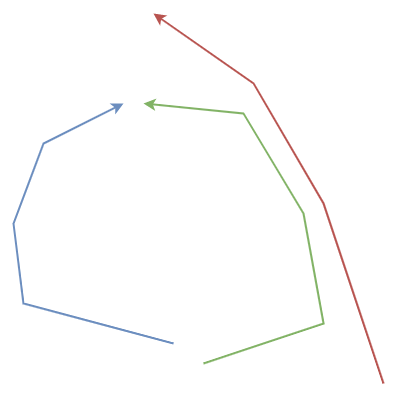
\includegraphics[width=0.5\textwidth]{images/argoverse-clcand-flaws.drawio.png}
  \caption{Пример где \textit{Argoverse} алгоритам за проналазак кандидата не даје тачне одговоре}
  \label{argoverse-clcand-flaws}
\end{figure}

Током тренирања \textit{VectorNet} модела који ће бити објашњен у наредној секцији, анализом података је примећено да је један од главних
разлога лошијих перформанси заправо слаб квалитет узорковања кандидата путних сегмената. Није ретко да се изабере путни сегмент који припада
супротној линији вожње и да због тога предикције буду јако лоше. Из тих разлога је одлучено да се имплементира једноставнији алгоритам
који се своди на коришћење \textit{DTW (Dynamic Time Warping)} методе и апроксимације угла између трајекторије и путног сегмента. приказан
је алгоритам \ref{dtw-algorithm} као \textit{Python} псеудокод.

\begin{figure}
  \begin{python}
  def dtw_algoritam(trajektorija, avm, dfs_radijus, putni_segmenti, 
      k = 3, max_ugao = 90):
    # trajektorija: istorija trajektorije agenta 
    # avm: Argoverse mapa (interfejs ka grafu mape)
    # dfs_radijus: uslov zaustavljanja dfs algoritma
    # putni_segmenti: koriste se putni segmenti dobijeni iz prethodnog koraka
    # k: broj najboljih putnih segmenata koji se uzimaju u obzir kao kandidati
    # max_ugao: Maksimalni ugao uzmedju trajektorije 
    #           i kandidata putnog segmenta
    
    # racuna se rastojanje putnog segmenta od trajektorije
    # koristi se dtw metoda sa L2 metrikom
    rastojanje_putni_segment = []
    for ps in putni_segmenti:
      rastojanje = dtw(trajektorija, ps)
      rastojanje_putni_segment.append((rastojanje, ps))

    # sortiranje po rastojanju
    rastojanje_putni_segment = sorted(rastojanje_putni_segment)
    # rastojanje vise nije bitno
    putni_segmenti = [ps for _, ps in rastojanje_putni_segment]
    putni_segmenti = putni_segmenti[:k]  # k najboljih

    # za svakog od putnih segmenata se pronalaze sledbenici dfs algoritmom
    kandidati = []
    for ps in putni_segmenti:
      sledbenici = avm.dfs(ps, dfs_radijus)
      kandidati.extend(sledbenici)

    kandidati = list(set(kandidati))  # uklanjanje duplikata

    # kandidati se filtriraju na osnovu ugla izmedju putnog segmenta
    # i trajektorije
    filtrirani_kandidati = []
    traj_pravac = izracunaj_pravac_trajektorije(trajektorija)
    traj_ugao = izracunaj_ugao_pravca(traj_pravac)
    for ps in kandidati:
      ps_pravac = izracunaj_pravac_trajektorije(ps)
      ps_ugao = izracunaj_ugao_pravca(ps_pravac)
      ugao = abs(traj_ugao - ps_ugao)
      if ugao > min_ugao:
        continue
      
      filtrirani_kandidati.append(ps)

    return filtrirani_kandidati

  \end{python}
  \caption{Алгоритам заснован на \textit{DTW} метрици и хеуристици угла између правца трајекторија \label{dtw-algorithm}}
  \end{figure}

Идеја је следећа: уместо да се узима у обзир само последња тачка, упоређују се све тачке путног сегмента и трајекторије 
(путни сегмент је такође трајекторија). Коришћење \textit{ADE} метрике није идеално за поређење временских серија, јер 
то подразумева јака ограничења за асоцијације тачака. Асоцијација тачака се односи на то која тачка прве трајекторије може 
да се упари са којом тачком друге трајекторије. У случају \textit{ADE} метрике, свака тачка прве трајекторије
може да се упари само са једном тачком друге трајекторије. Метода \textit{DTW} одбацује то ограничење и омогућава
да свака тачка једне трајекторије може да се упари са било којом тачком друге трајекторије. Остају ограничења да једна
тачка једне трајекторије може да се упари са највише једном тачком друге трајекторије (а може и мање) и 
немогуће је испреплетано упаривање (ако се тачка 5 упари са тачком 8, онда тачка 4 не може да се упари са тачком 9). Метода
\textit{DTW} има разне примене над временским серијама, а алгоритам је уопштење Левенштајновог растојања за ниске. На слици
\ref{euclidean_vs_dtw} се илуструје начин функционисања методе. У алгоритму се узима најбољих $K_c$ кандидата пре примене 
\textit{DFS}-a.

\begin{figure}[H]
  \centering
  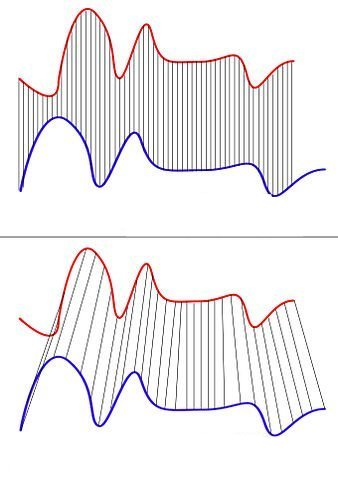
\includegraphics[width=0.5\textwidth]{images/Euclidean_vs_DTW.jpg}
  \caption{Упоређивање серија помоћу класичног еуклидског растојања (горе) и \textit{DTW} методе (доле)}
  \label{euclidean_vs_dtw}
\end{figure}

Упоређивање трајекторија на овај начин није довољно. Проблем прави трајекторија агента на сценама где се он не креће или се веома споро креће. Пошто
се \textit{DTW} своди на еуклидско растојање са флексибилнијим асоцијацијама тачака, 
онда у случају да трајекторија агента има приближан облик тачке, долази до упаривања са најближим путним сегментом уместо са идеалним. Додатни проблем 
код овог приступа је
то што је путни сегмент одређен централном трајекторијом и ако агент није потпуно усклађен са његовим путним сегментом (нпр. искаче мало
из своје траке), онда је 
најближи путни сегмент заправо онај суседни који има супротну траку. Узимање путног сегмента са супротном траком је катастрофално,
јер применом \textit{DFS}-а се врши претрага у потпуно погрешном смеру. Због тога се додаје хеуристика која упоређује углове између
трајекторија кандидата путних сегмената добијених \textit{DTW} методом и угла трајекторије агента. Угао се одређује као угао вектора правца
трајекторије, а вектор правца је одређен првом и последњом тачком трајекторије. Уколико је угао између трајекторије агента и 
трајекторије путног сегмента већи од $\theta_{min}$ степени, онда се тај путни сегмент одбацује. За $K_c$ се узима вредност 3, а
за $\theta_{min}$ се узима вредност 90.

Коначан векторизован облик је димензије $N_c\times N_r\times 3$, где је $N_c$ број пронађених кандидата,
$N_r$ дужина трајекторије реализације. Пошто се путеви допуњавају по потреби до димензије $N_r$, користи се трећа координата
за маску која има вредност 0 ако је пут допуњен, односно 1 ако пут није допуњен. 

\section{Визуализација сценарија}

На сликама \ref{scenario-example-MIA-148229}, \ref{scenario-example-MIA-16518}, \ref{scenario-example-PIT-20617} и \ref{scenario-example-PIT-146292} 
се налазе примери визуализованих сценарија након иницијалне припреме. На сваком сценарију су приказани елементи обојени посебном бојом:
\begin{itemize}
  \item Путни сегменти обојени сивом бојом;
  \item Историја трајекторије агента обојена тамно зеленом бојом;
  \item Истинита вредност трајекторије агента која се предвиђа обојена светло зеленом бојом;
  \item Историја трајекторија свих суседа (осталих покретних објеката на сцени) обојена наранџастом бојом;
  \item Истинита вредност трајекторије суседа чији се временски интервал поклапа са истинитом вредношћу трајекторије агента обојена жутом бојом;
  \item Кандидати путних сегмената обојени црном бојом и приказани испрекиданим линијама.
\end{itemize}

Кандидати путних сегмената након примене \textit{DFS} хеуристике су јако прецизни и у већини случајева су квалитета као на
сликама \ref{scenario-example-MIA-148229}, \ref{scenario-example-MIA-16518} и \ref{scenario-example-PIT-20617}. Сценарио 
\ref{scenario-example-PIT-146292} је издвојен као проблематичан пример како би се приближније приказала мана \textit{DTW} хеуристике.
У екстремном случају када агент мирије и трајекторија има облик тачке, примена \textit{DTW} метрике са еуклидским растојањем се своди на
проналазак најближе трајекторије тј. као да се само користи еуклидско растојање, што врло вероватно проналази погрешног кандидата за путни сегмент.
У овом случају агент има спор старт, па је трајекторија збијена и има облик тачке. Због облика се историја трајекторије агента (зелена линија)
упарује са најближим и најкраћим путним сегментима у околини, што је у овом случају изабрани кандидат за путни сегмент.

\begin{figure}[H]
  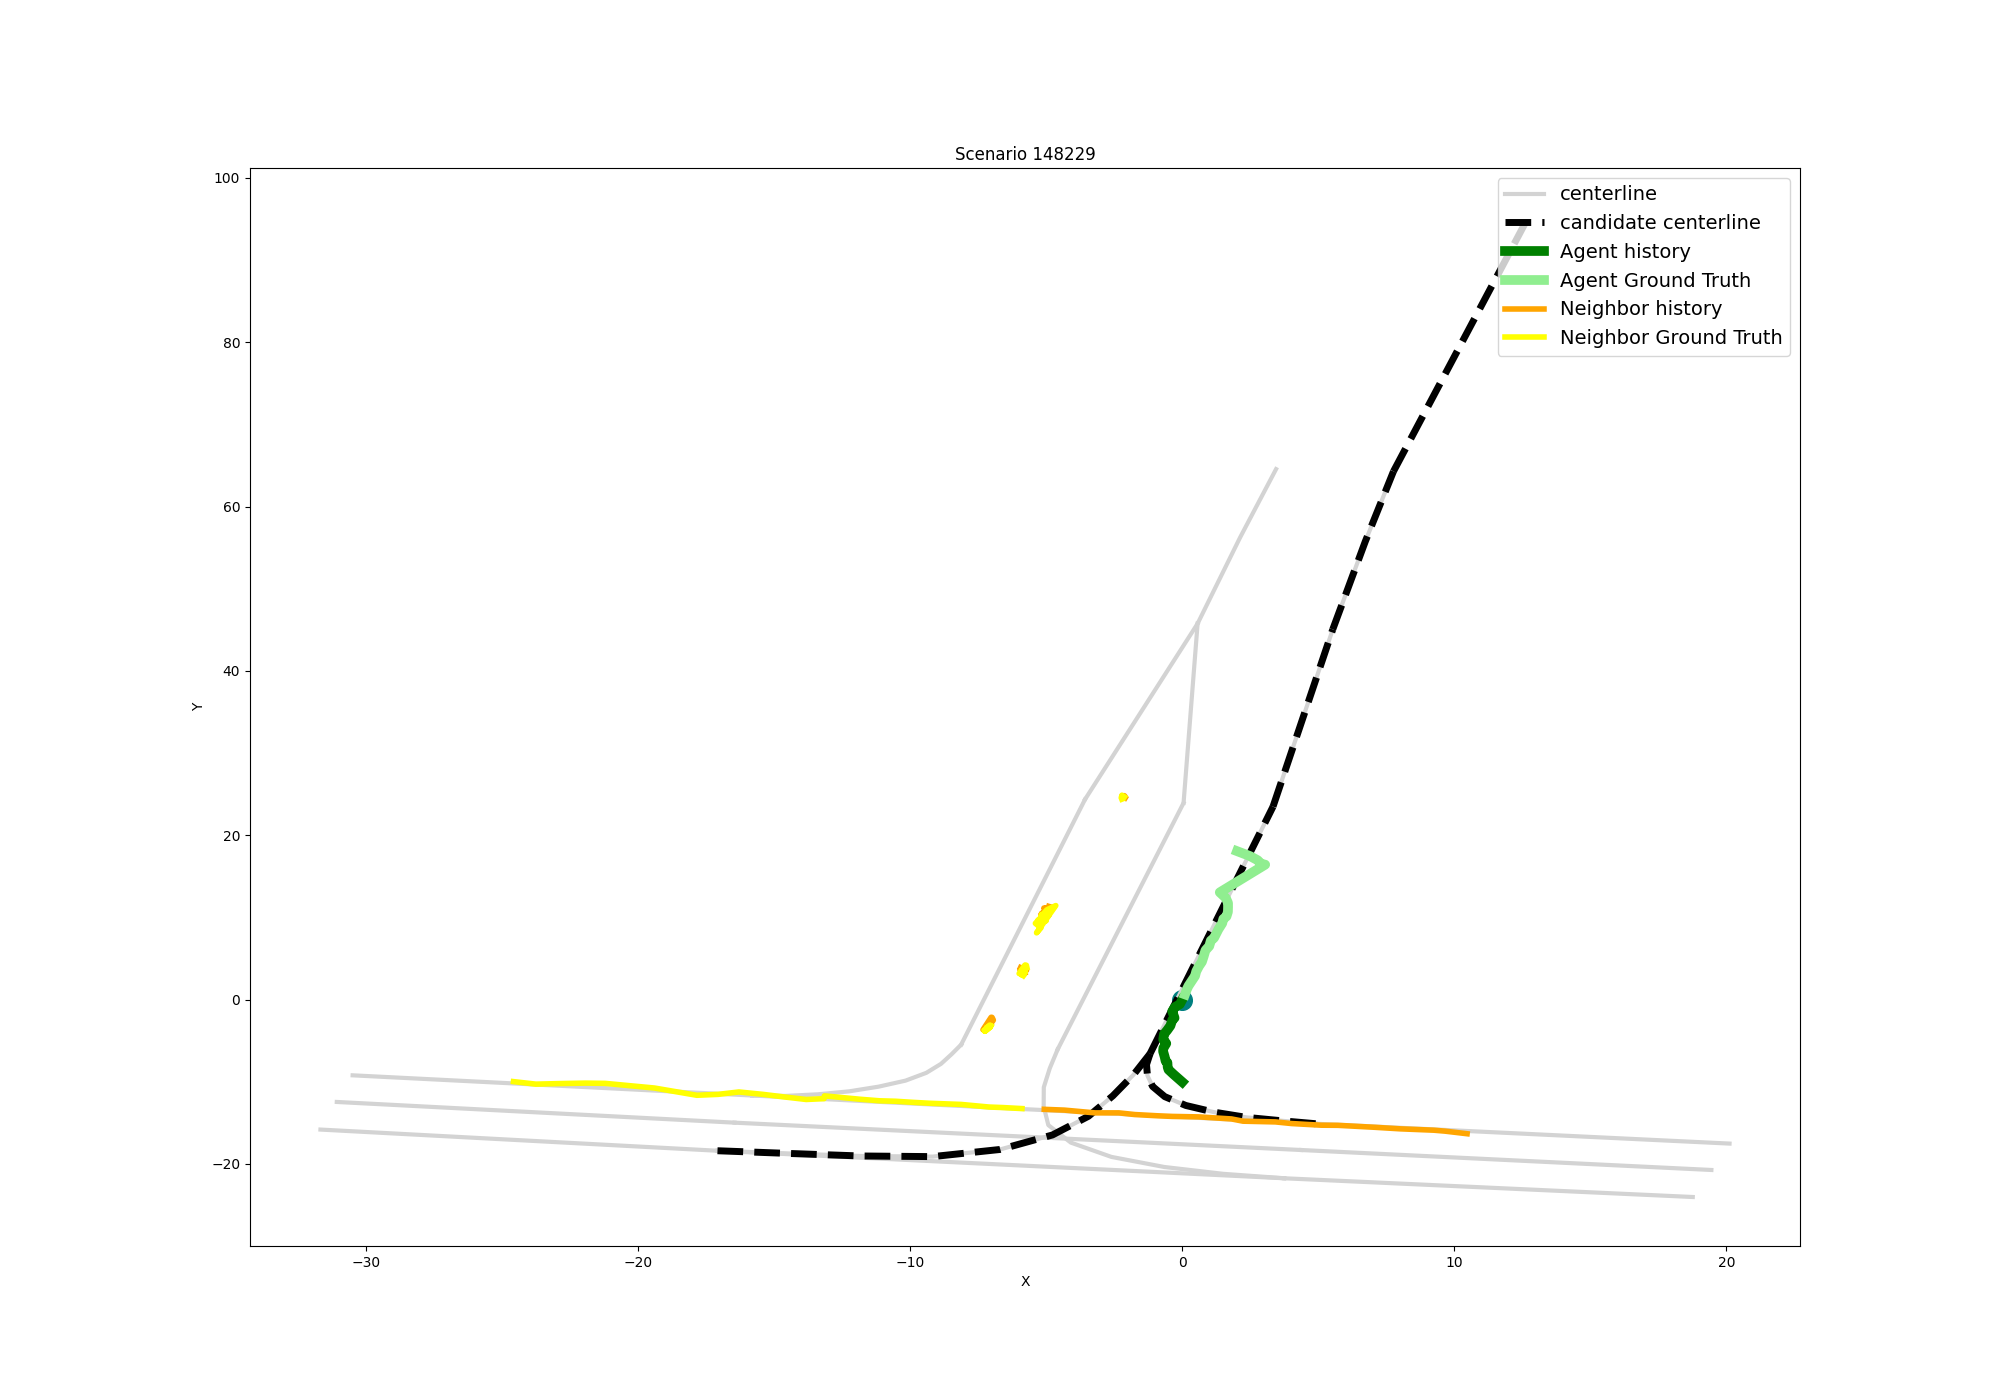
\includegraphics[width=0.9\textwidth]{images/scenario_MIA_148229.png}
  \caption{Визуализација припремљених података - \textit{MIA 148229}}
  \label{scenario-example-MIA-148229}
\end{figure}

\begin{figure}[H]
  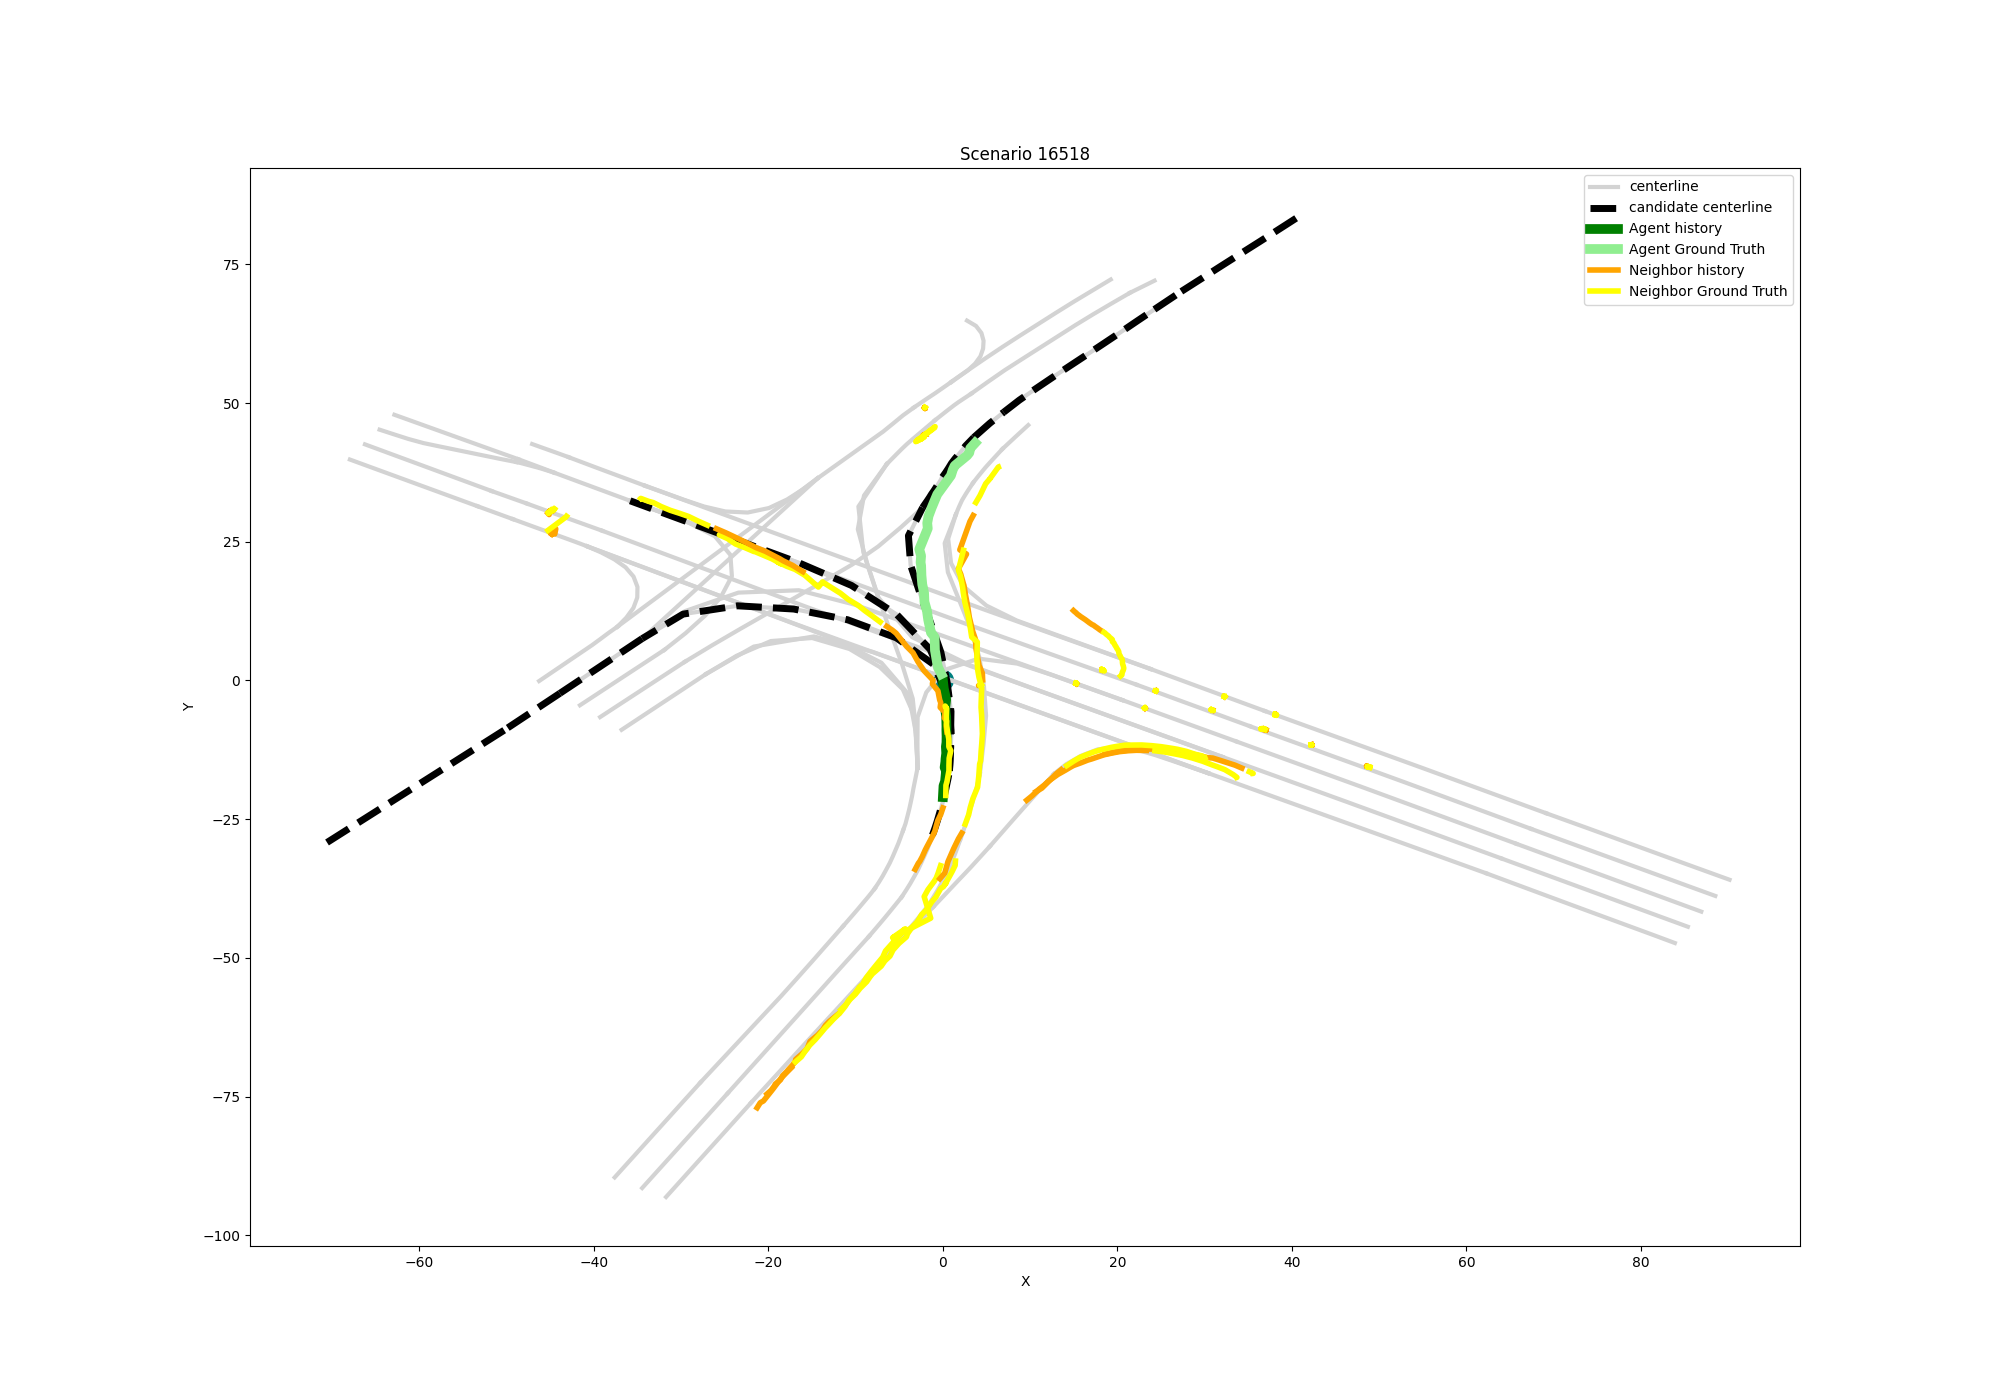
\includegraphics[width=0.9\textwidth]{images/scenario_MIA_16518.png}
  \caption{Визуализација припремљених података - \textit{MIA 16518}}
  \label{scenario-example-MIA-16518}
\end{figure}

\begin{figure}[H]
  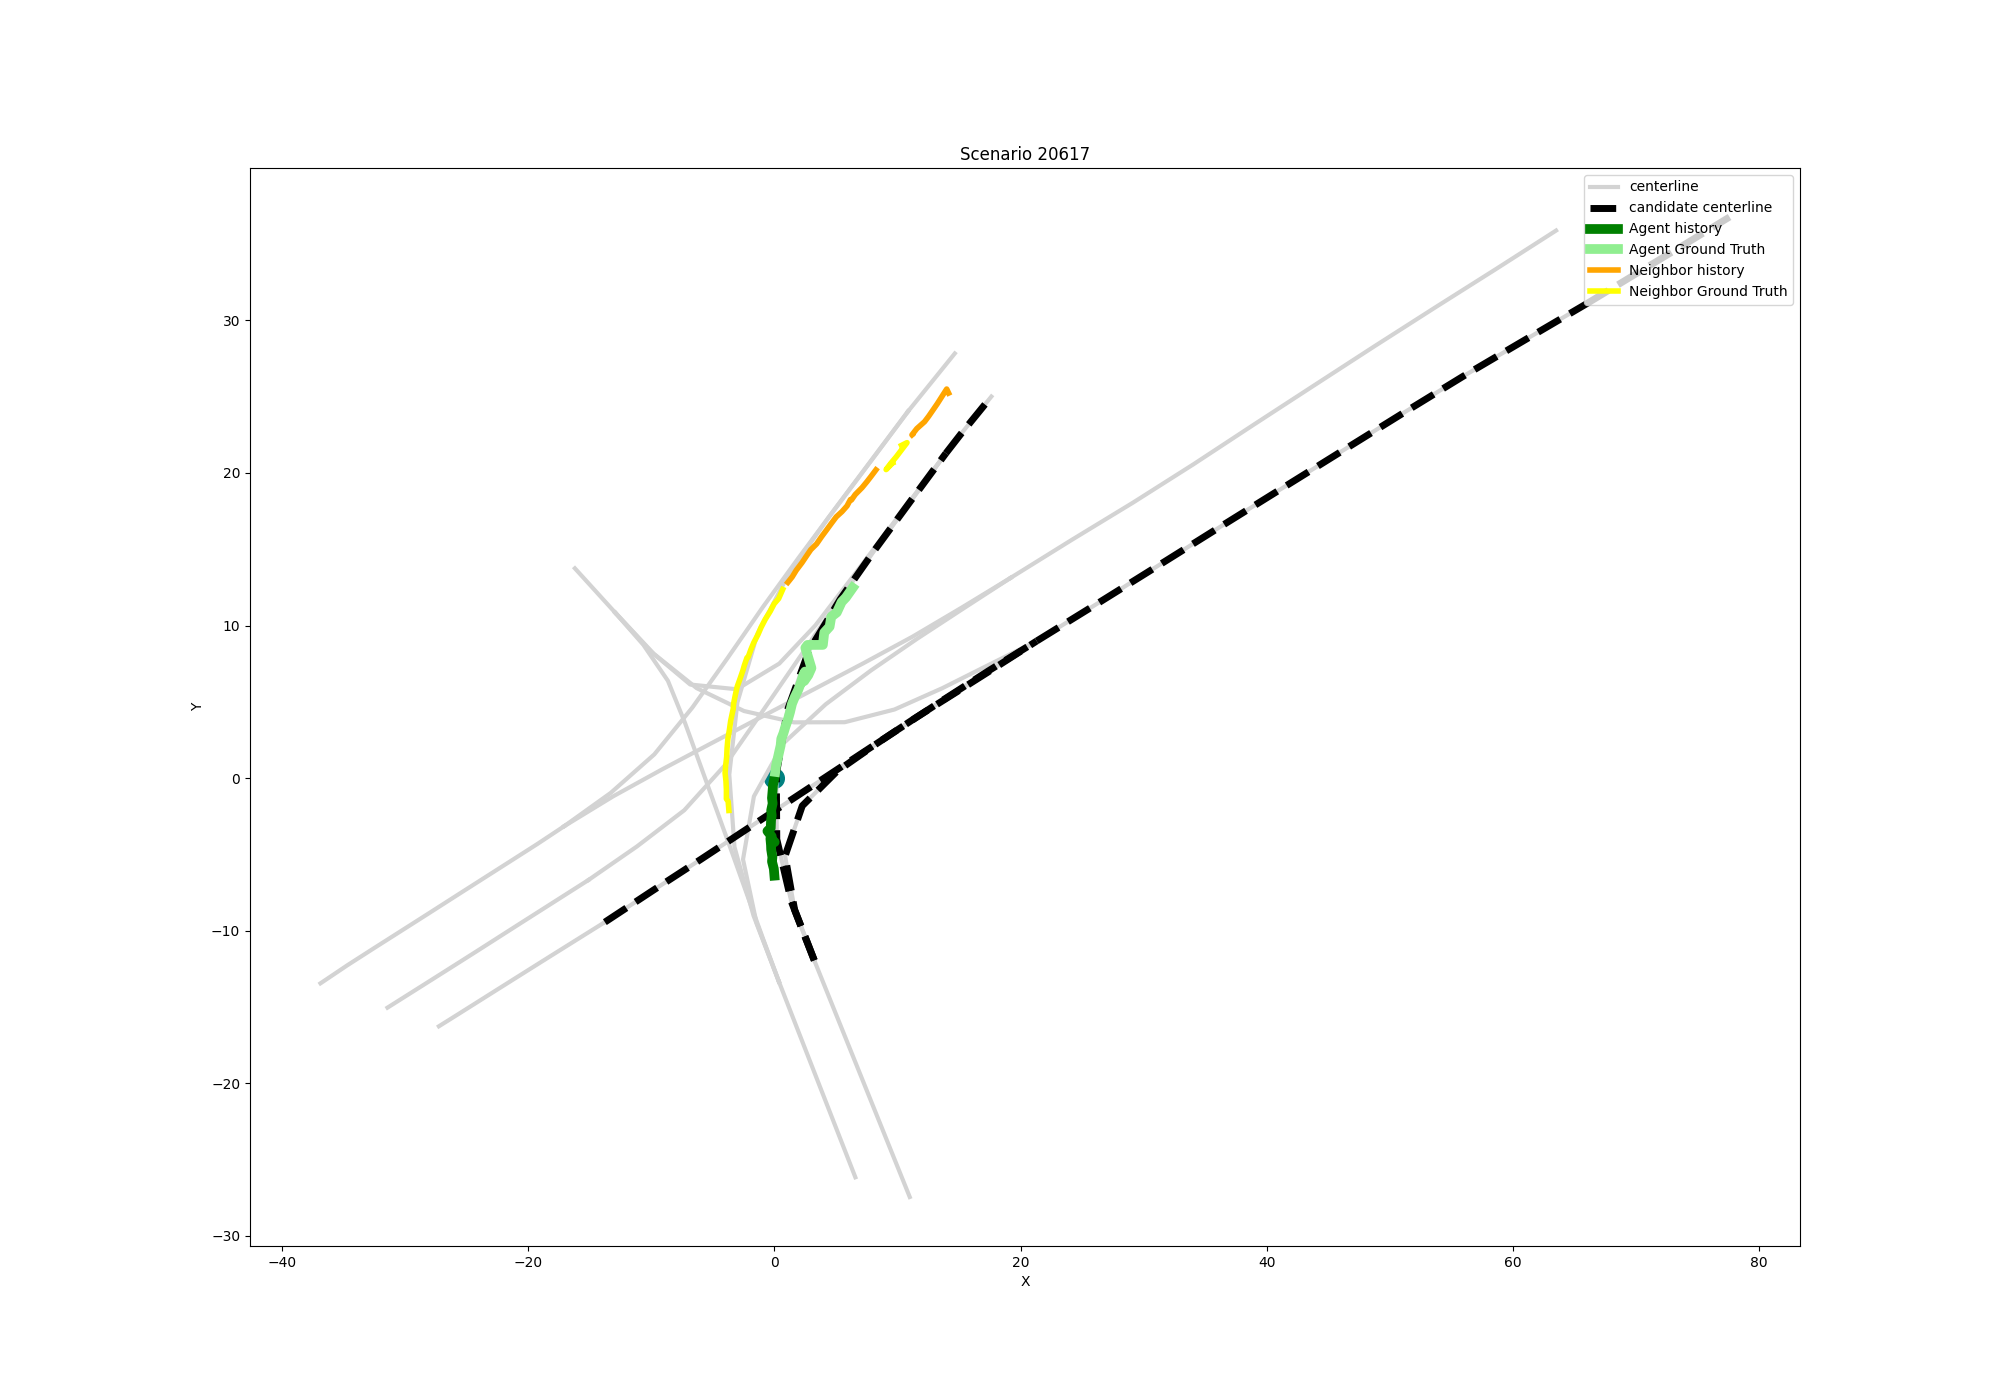
\includegraphics[width=0.9\textwidth]{images/scenario_PIT_20617.png}
  \caption{Визуализација припремљених података - \textit{PIT 20617}}
  \label{scenario-example-PIT-20617}
\end{figure}

\begin{figure}[H]
  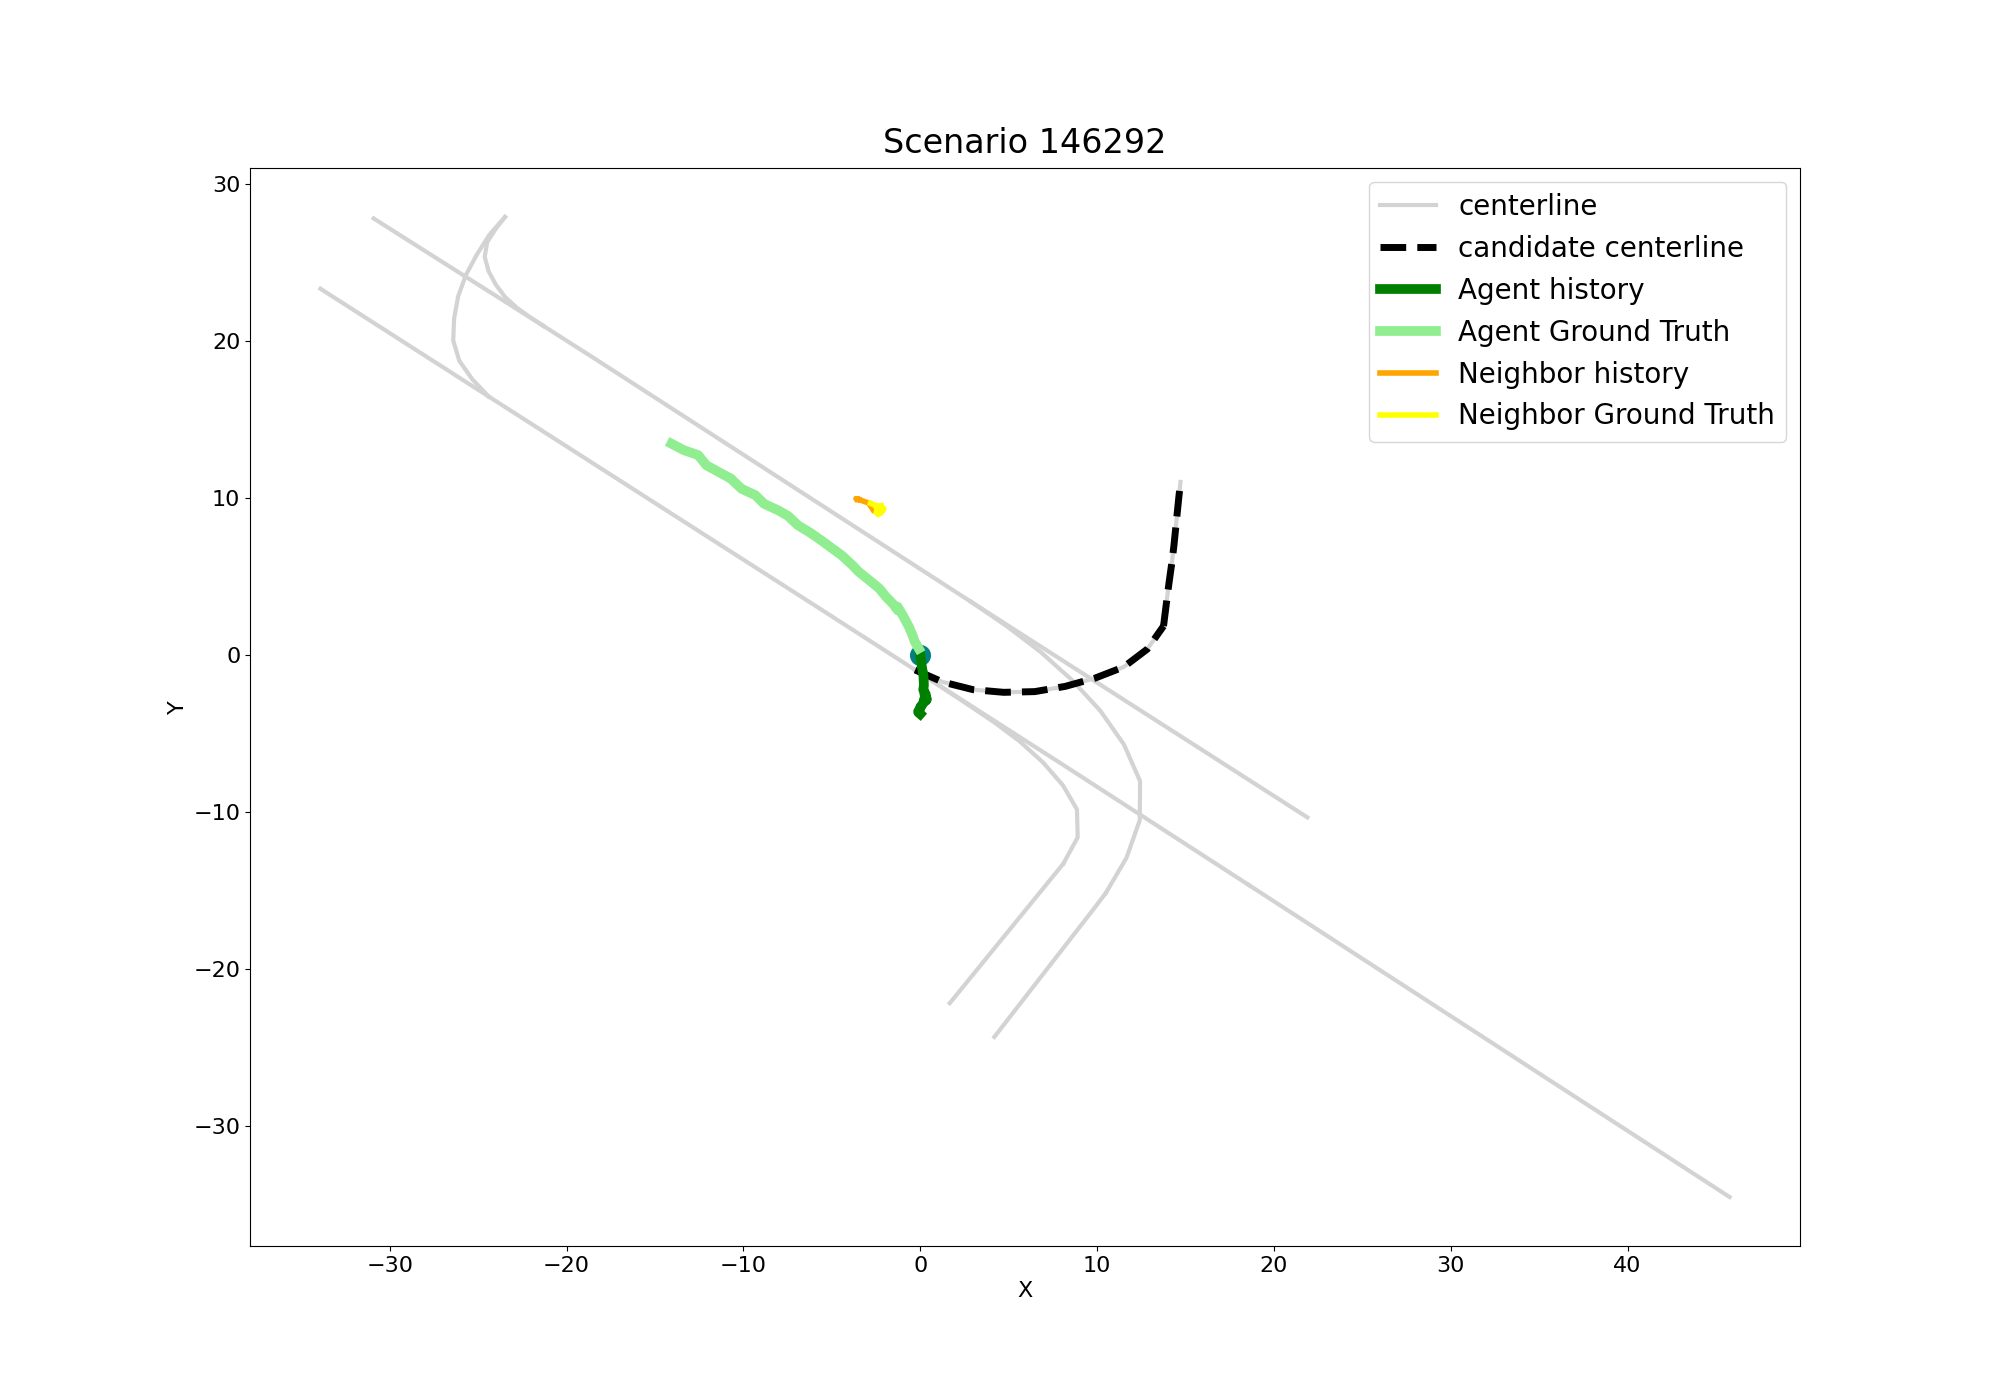
\includegraphics[width=0.9\textwidth]{images/scenario_PIT_146292.png}
  \caption{Визуализација припремљених података - \textit{PIT 146292}}
  \label{scenario-example-PIT-146292}
\end{figure}

% ------------------------------------------------------------------------------
\chapter{Техника заснована на разумевању контекста обрадом сцене представљене графом}
\label{chp:razrada}
% ------------------------------------------------------------------------------

Независно од конкретног скупа података \textit{HD} мапа, сваки сценарио може да се представи графовском структуром која повезује тачке на сцени, где
свака тачка има своја својства. Свака трајекторија може да се посматра као усмерена сложена отворена линија (\textit{eng. polyline}) тј.
низ тачака таквих да су сваке две суседне тачке у низу спојене једном усмереном дужи. Тој сложеној линији одговара граф у којем свака тачка
чини чвор, а усмерене дужи чине гране. Како већина елемената \textit{HD} мапа може да се представи сложеном линијом, граф чини идеалну структуру
за представљање једног сценарија. Граф може да се посматра на два нивоа, где се први, нижи ниво односи на топологији сложених линија, а други, виши ниво 
се односи на на везе између сложених линија тј. сложене линије чине чворове у том графу. На овај начин је дефинисана хијерархија графа. 
У наставку се граф на првом нивоу назина подграф, а граф веза између сложених линија се назива глобални граф интеракција (односи се на интеракције
између различитих сложених линија на сцени).

Сценарио из \textit{Argoverse} скупа података се састоји из трајекторија агента, трајекторија суседа, путних сегмената и кандидата путних сегмената.
Како путни сегмент чини специјалну врсту трајекторија, јасно је да сви елементи сценарија могу да се представе сложеним линијама, а самим тим
цео сценарио може да се представи као претходно поменути граф. На слици \ref{polylines-representation} се налази пример једног сценарија
представљен преко сложених линија.

\begin{figure}[H]
  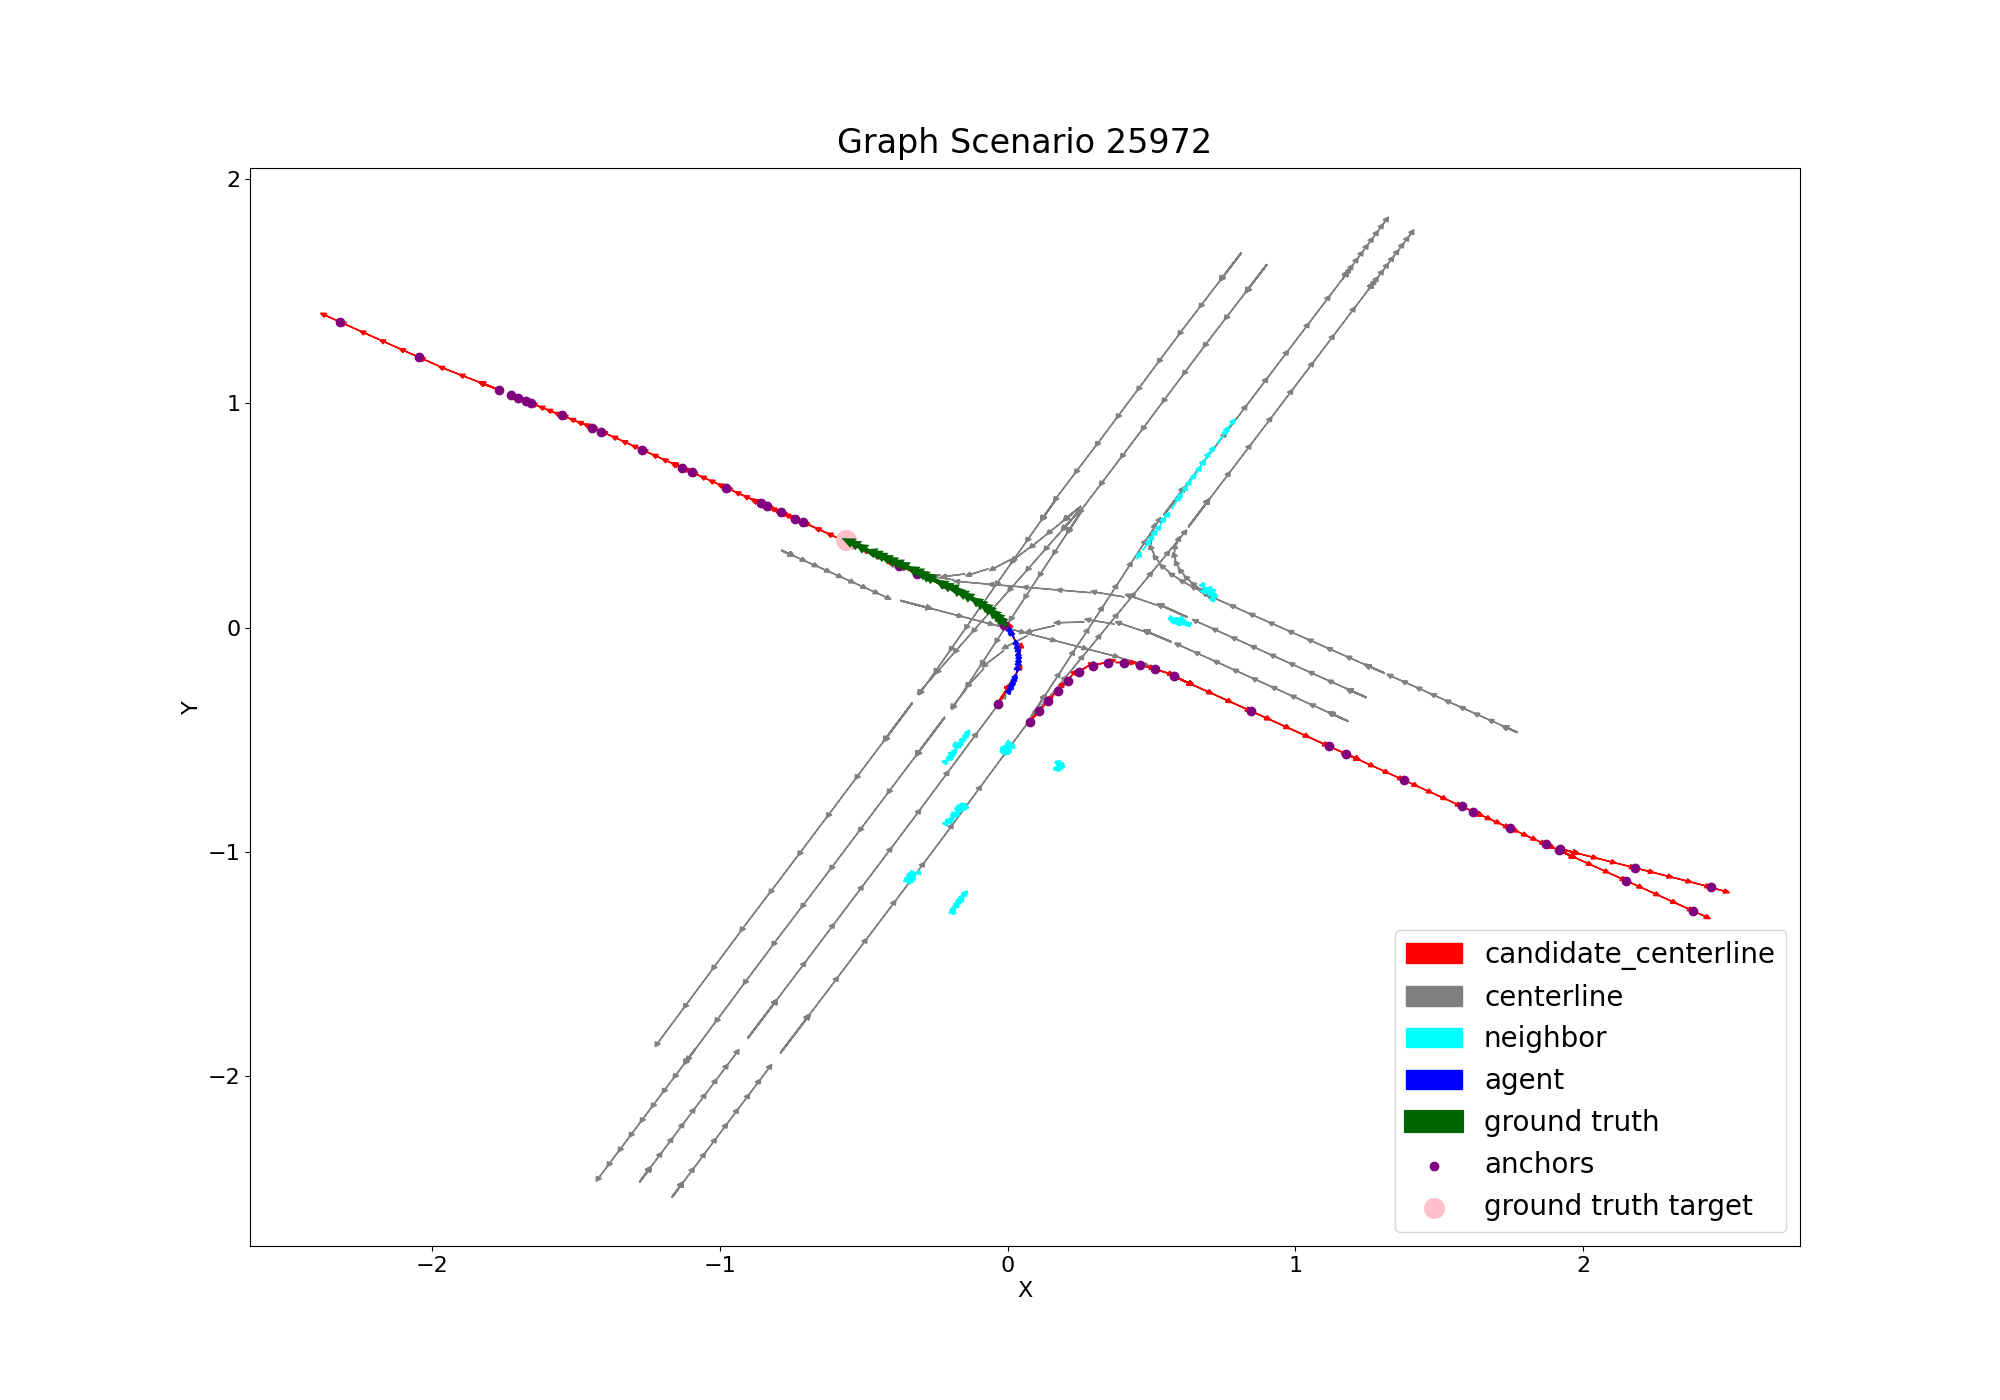
\includegraphics[width=1.0\textwidth]{images/polylines-representation.png}
  \caption{Визуализација репрезентације сложеним линијама}
  \label{polylines-representation}
\end{figure}

\section{Припрема података}

Припрема података у овој секцији се наставља на иницијални процес припреме података и своди се на трансформацију свих елемената
\textit{HD} мапа у сложене линије. Да би било могуће спојити више сценарија у један подскуп података (\textit{eng. batch}) 
за једну итерацију тренирања, неопходно је да се испуне одређени услови:
\begin{itemize}
  \item Сваки сценарио мора да има исти број сложених линија ($N_{p}$). Ако је број сложених линија већи од $N_{p}$, онда се 
        вишак сложених линија одбацује, при чему се води рачуна о приоритету сложених линија: агент, остали објекти, путеви, путеви кандидати.
        Ако је број сложених линија мањи од $N_{p}$, онда се скуп допуњава сложеним линијама са нула чворовима.
  \item Свака сложена линија мора да има исти број чворова ($N_{n}$). Ово се решава аналогно броју сложених линија.
  \item Сваки чвор сложених линија мора да има исти број својстава ($N_{f}$). Сваки чвор има иста својства, са тим
        да се својства допуњавају нулама ако немају смисла за тај тип сложених линија (агент и путни сегменти немају иста својства).
\end{itemize}

\noindent Сваки чвор сложене линије има следећа својства:
\begin{itemize}
  \item Координате \textit{x} и \textit{y}: просек претходне и тренутне тачке трајекторије - 2 скалара;
  \item Смер по \textit{x} и \textit{y}: разлика тренутне и претходне тачке трајекторије - 2 скалара;
  \item Тип објекта као \textit{onehot} вектор (агент, сусед - објекат, пут, пут кандидат) - 4 скалара;
  \item Метаподаци путних чворова (нуле у случају трајекторија агента и објеката суседа, јер то нису путни сегменти
        и метаподаци путних сегмената не важе за агенте и суседе)
    \begin{itemize}
      \item Да ли се сегмент пресеца са неким другим сегментом - 1 скалар;
      \item Да ли постоји контрола саобраћаја - 1 скалар;
      \item Смер као \textit{onehot} вектор (нема, десно, лево) - 3 скалара
    \end{itemize}
  \item Да ли је чвор прави (1) или вештачки (0) - 1 скалар (вештачки чвор се додаје да би сваки
        изабран подскуп подака имао исту димензију векторске репрезентације.).
\end{itemize}

Коначан формат улазних података у \textit{VectorNet} је $B\times N_{p}\times N_{n}\times 14$, где је $B$ број сценарија у једном подскупу података,
а $N_{p}$ и $N_{n}$ су параметри. За сам \textit{VectorNet} модел је довољно да се сви елементи трансформишу у скуп сложених линија. За
\textit{TNT-VectorNet} варијанту је потребно да се узоркују предлози крајњих тачака на основу кандидата путних сегмената. 

\subsection{Узорковање предлога крајњих тачака из кандидата путних сегмената}

У кораку иницијалне припреме у глави \ref{initprep} су одређени кандидати путних сегмената. Циљ скупа кандидата путних сегмената је да се применом доменског знања
одреде сви могући путеви где се очекује да агент у будућности може да се креће. Узорковање предлога крајњих тачака трајекторије агента се врши над
скупом тих кандидата путних сегмената. Величина узорка $N_{ep}$ се унапред дефинише и чини хиперпараметар припреме података. Нека је величина скупа
кандидата путних сегмената једнака $N_{crs}$. Тада се узоркује $\frac{N_{ep}}{N_{crs}}$ тачака са сваког путног сегмента. Разлика броја
узоркованих тачака са два путна сегмента није већа од 1. Након тога се за сваки путни сегмент узоркују тачке униформно. 

Путни сегмент је представљен као сложена линија $A_{1}A_{2}...A_{n}$ тј. низ дужи. Свака дуж $AB$ може да се параметризује као 
$r(t) = A + t\cdot \vec{AB},\ t \in [0, 1]$. Аналогно томе, сложена линија може да се параметризује тако што се параметризује свака дуж која њој припада,
а ограничење на параметар $t$ сложене линије се поставља тако да важи $t \in [0, n]$ ($n$ je дужина сложене линије), где се цео део параметра $t$ односи индекс дужи, а децимални
део се односи на позицију у оквиру те дужи. Ако се сложена линија овако параметризује, онда је униформно узорковање еквивалентно еквидистантном узорковању
параметра $t$. 

Мана овог алгоритма су "нагомилане" узорковане тачке за неке делове сложене линије. Ово је последица чињенице да путни сегменти у \textit{Argoverse} 
скупу података не садрже дужи приближно једнаке дужине и понекад пар дужи чини већину дужине сложене линије тј. путног сегмента. 

Приказана су два примера \ref{poly-MIA-189984}, \ref{poly-MIA-32197} визуализације трансформисане сцене са узоркованим крајњим тачкама трајекторије агента:
\begin{itemize}
  \item Сивом бојом су обојене сложене линије путних сегмената; 
  \item Tамно плавом бојом је обојена сложена линија историје агента; 
  \item Светло плавом бојом су обојене сложене линије суседних објеката на сцени;
  \item Зеленом бојом је обојена истинита вредност трајекторије агента;
  \item Црвеном бојом су обојене сложене линије кандидата путних сегмената;
  \item Мали љубичасти кругови представљају узорковане тачке;
  \item Велики розе круг представља истиниту крајњу тачку агента.
\end{itemize}

\begin{figure}[H]
  \centering
  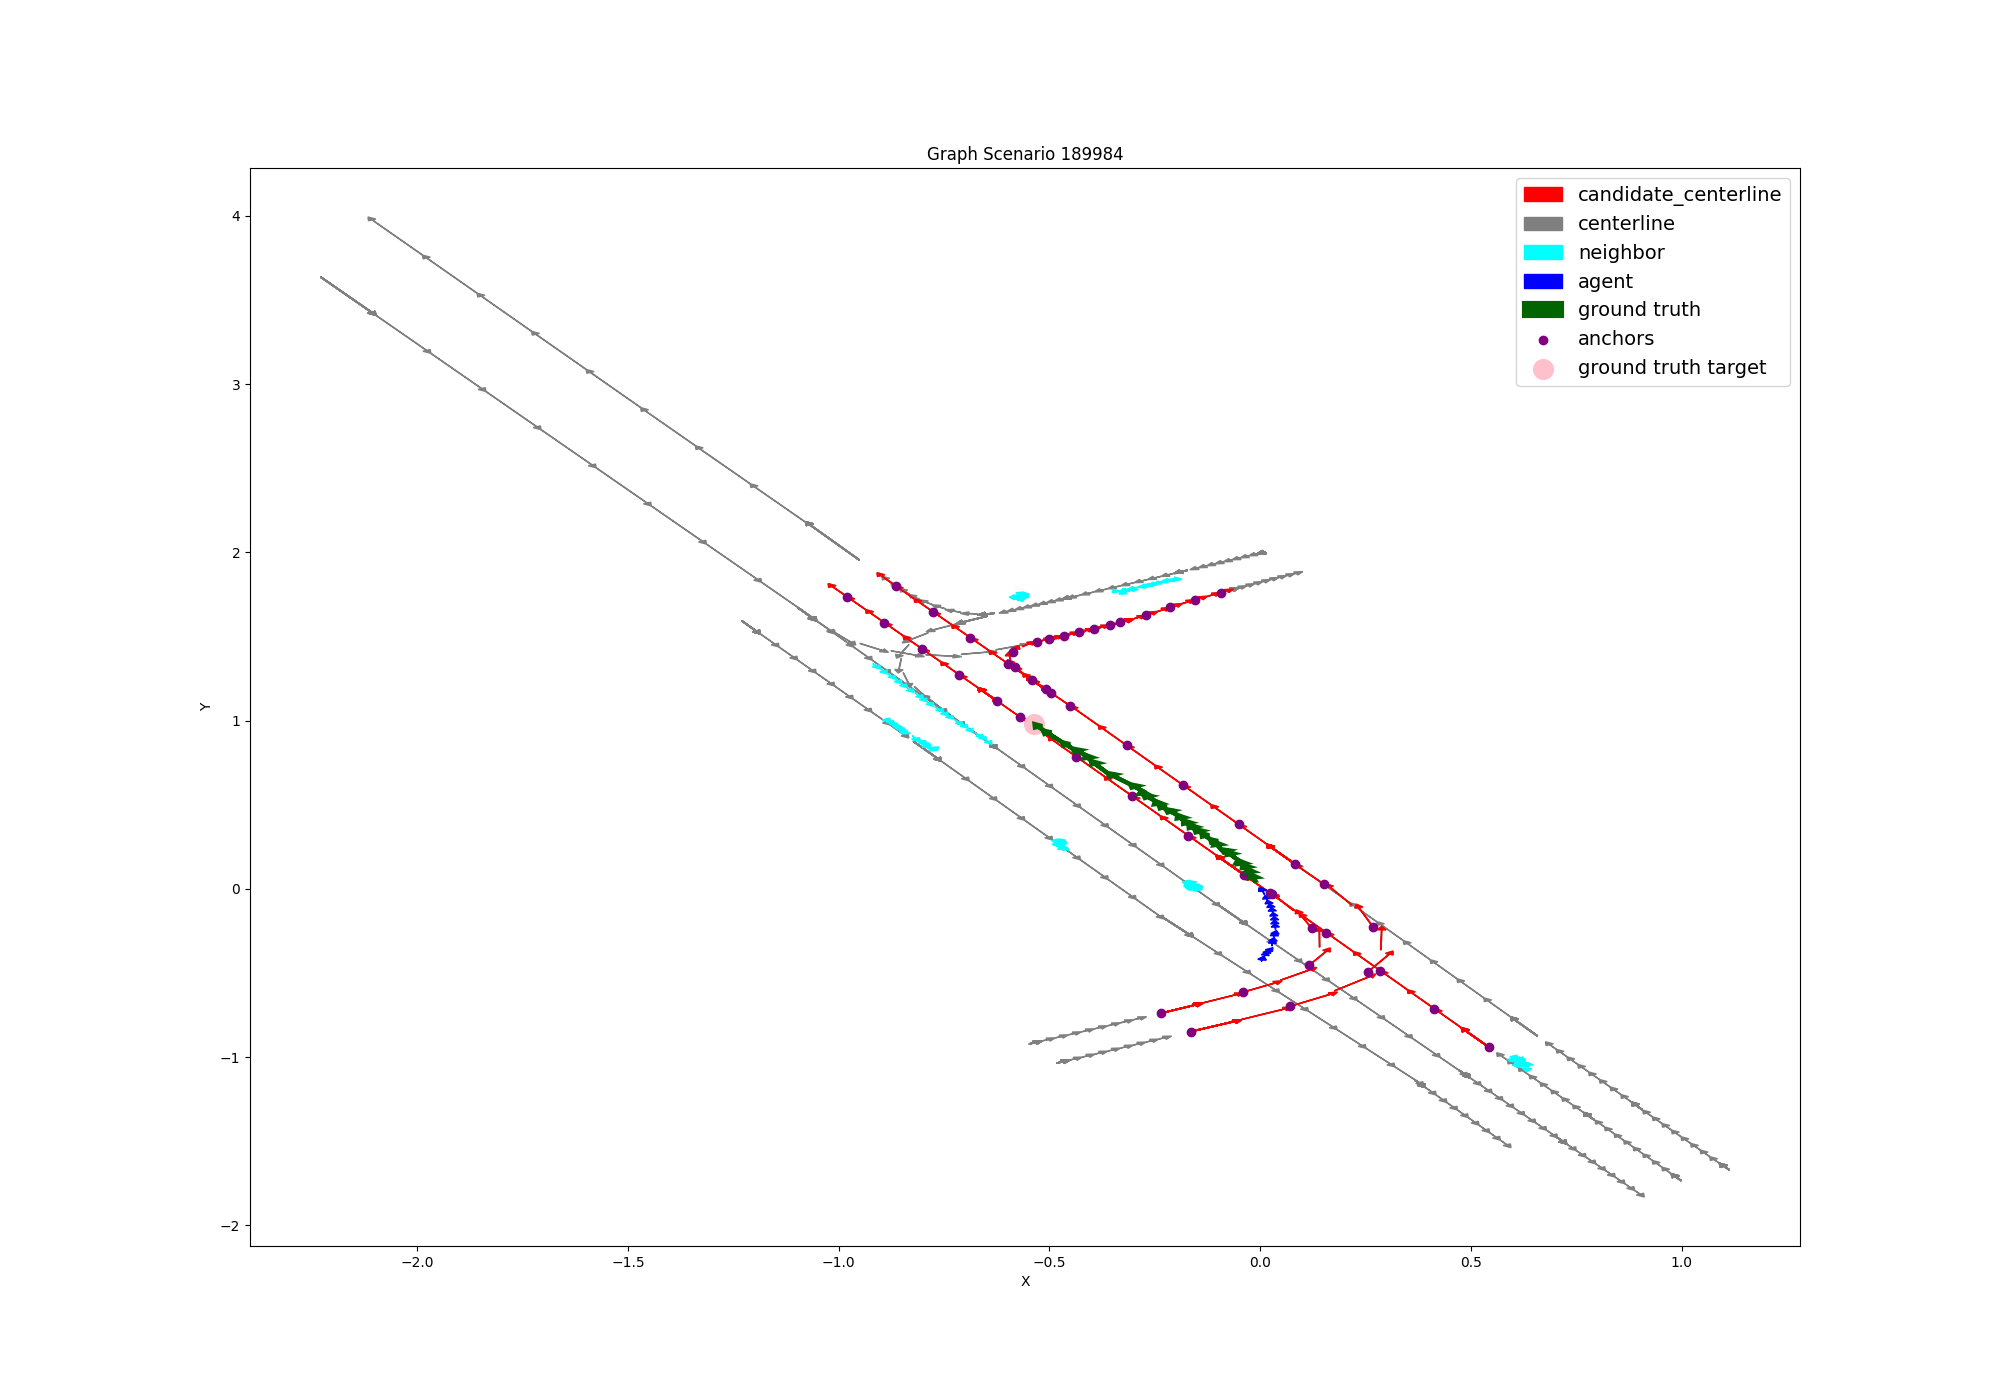
\includegraphics[width=0.9\textwidth]{images/polylines_MIA_189984.png}
  \caption{Визуалиција сложених линија - \textit{MIA 189984} \label{poly-MIA-189984}}
\end{figure}

\begin{figure}[H]
  \centering
  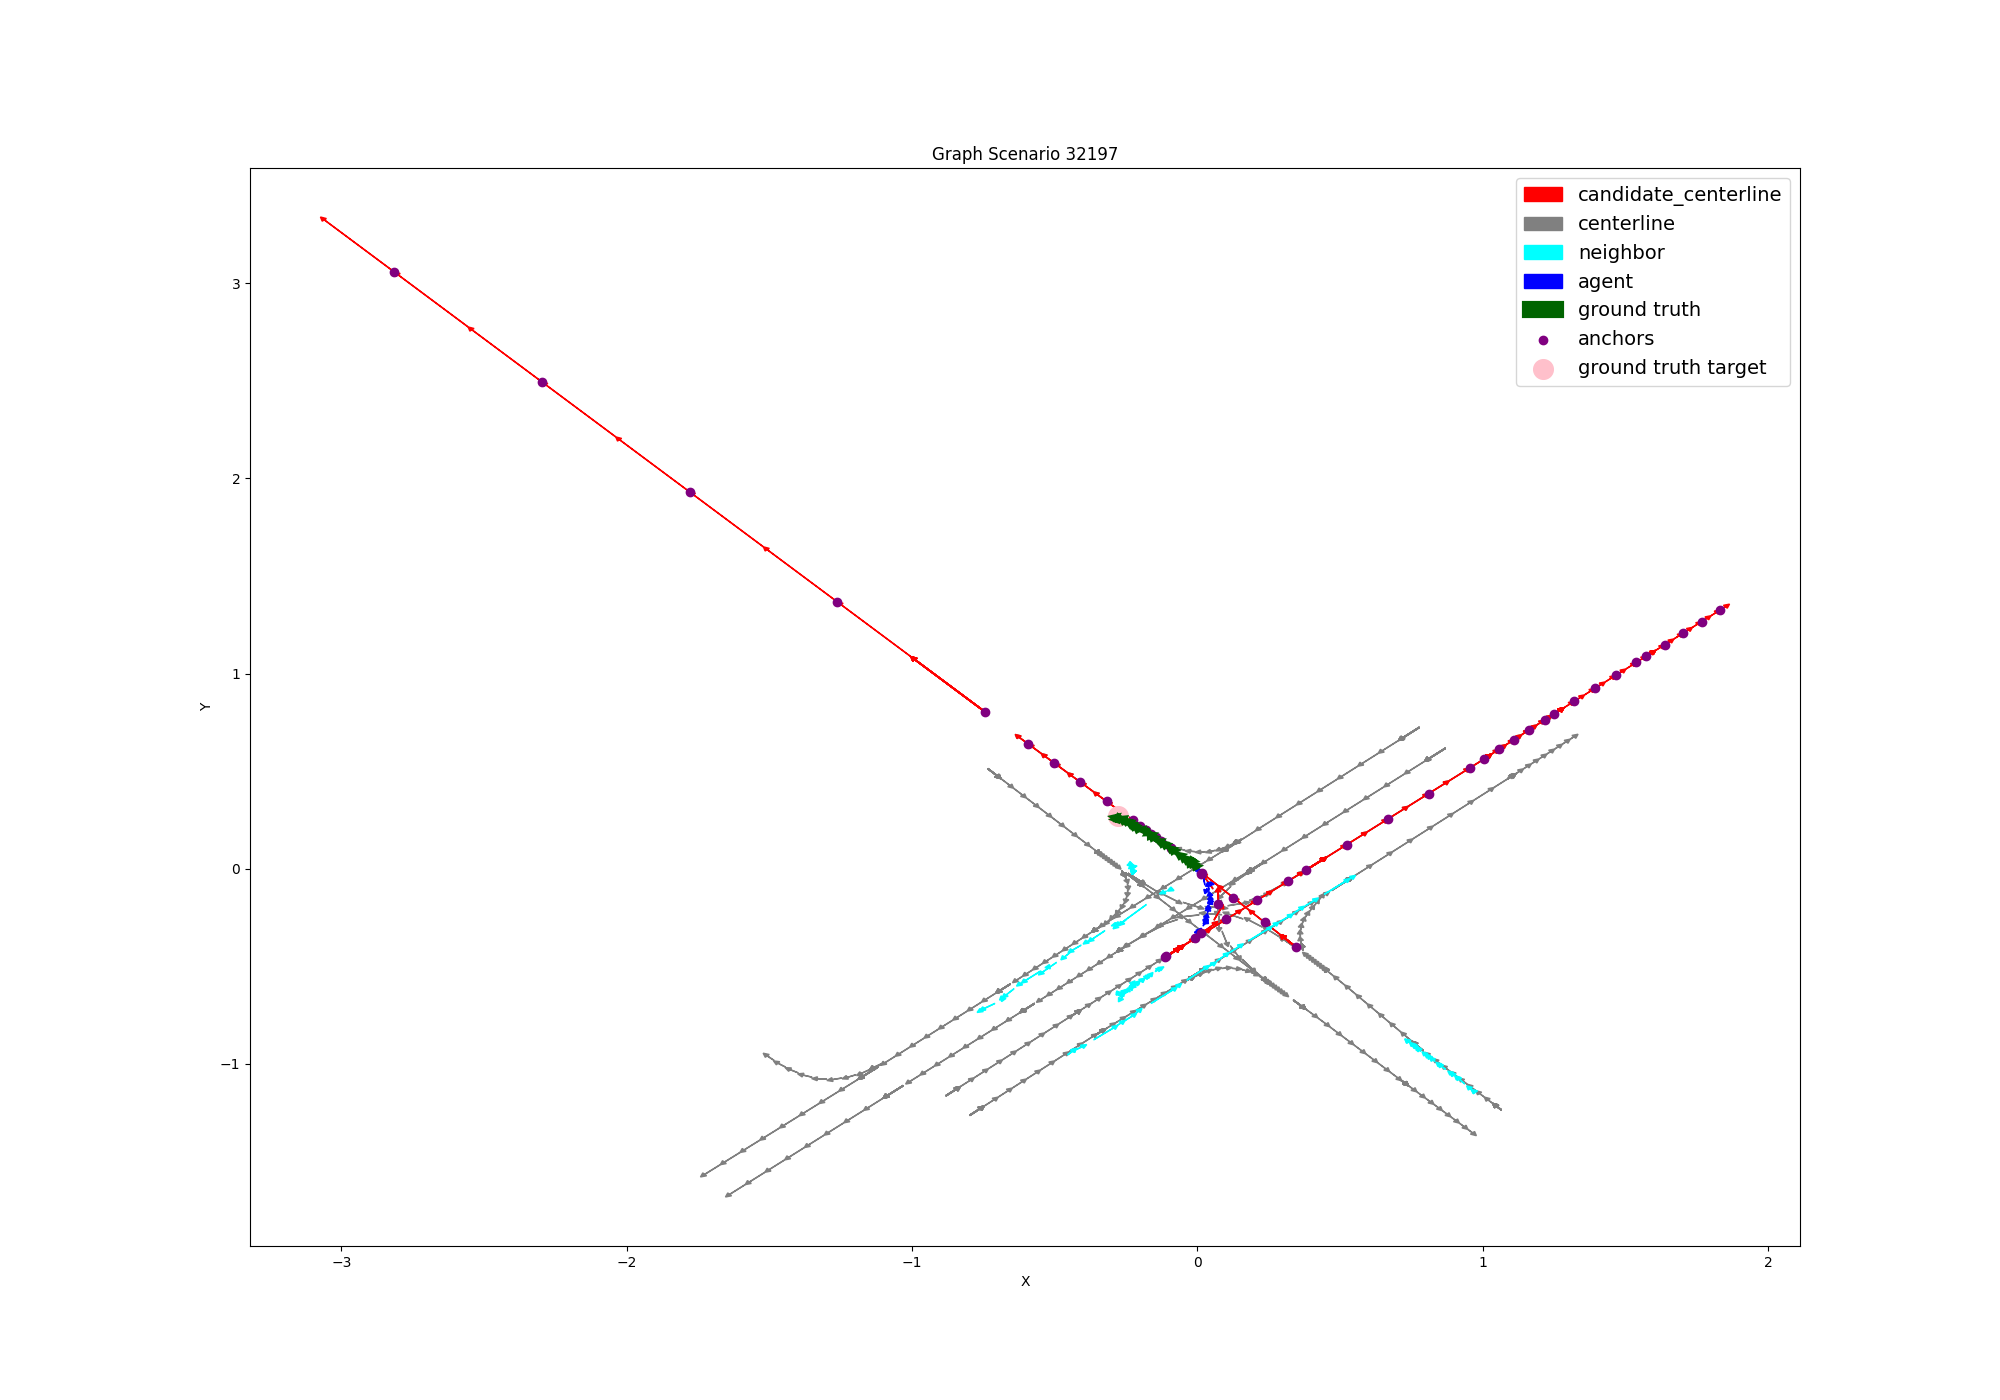
\includegraphics[width=0.9\textwidth]{images/polylines_MIA_32197.png}
  \caption{Визуалиција сложених линија - \textit{MIA 32197} \label{poly-MIA-32197}}
\end{figure}

\section{Модел \textit{VectorNet}}

\textit{VectorNet} је хијерархијска графовска неуронска мрежа која као улаз добија претходно дефинисани граф на два нивоа, а као резултат
даје предвиђања трајекторија за све изабране агенте. Архитектура може да генерише предикције за више агената у исто време. То
је погодно искористити у случају да координатни систем сценарија није већ прилагођен конкретном агенту. У супротном је погодније
да се користи итеративни приступ генерисања предикција.

У наставку ове и осталих секција ће бити описана комплетна архитектура и начин тренирања ове неуронске мреже. Модел се састоји из три компоненте,
чији називи одговарају структури комплетног графа који се користи \cite{vectornet}:
\begin{itemize}
  \item Подграф: агрегација сложених линија у један вектор који се даље посматра као чвор у глобалном графу;
  \item Глобални граф интеракција: моделовање интеракција на високом нивоу у глобалном графу помоћу механизма пажње;
  \item Предвиђање трајекторија за чворове глобалног графа који одговарају агентима.
\end{itemize}

\subsection{Подграф}

Свака сложена линија на сцени се посматра као посебан подграф. Применом графовске неуронске мреже
се издвајају битна својства и везе између чворова. Резултат се на крају агрегира како би се добио један вектор који представља репрезентацију те сложене линије.

Модел подграфа је варијанта \textit{GCN} архитектуре \cite{gcn} са више слојева. Визуализација једног слоја се види на слици \ref{vectornet-subgraph}. 
Сваки слој може да се представи следећом формулом:

\begin{figure}[H]
  \centering
  $v^{(l+1)}_{i} = \rho_{rel}(g_{enc}(v^{(l)}_{i}),\ \rho_{agg}(A, \{g_{enc}(v^{(l)}_{j})\})))$
\end{figure}

Овде је $v^{(l)}_{i}$ вектор својства чвора из претходног слоја ($v^{(0)}_{i}$ су улазна својства), $g_{enc}$ слој за кодирање
својства чвора, $\rho_{agg}$ операција агрегације порука добијених од суседних чворова, $A$ je матрица повезаности сложене линије, 
а $\rho_{rel}$ операција обједињавања агрегираних порука суседа и својства самог чвора. Конкретни избори
који се користе у овом раду су \cite{vectornet}:
\begin{itemize}
  \item $g_{enc}$ је потпуно повезана неуронска мрежа;
  \item $\rho_{agg}$ је максимум свих порука од суседа (\textit{maxpool});
  \item $\rho_{rel}$ је конкатенација својста чвора и агрегираних порука;
  \item \textit{A} је у оригиналном раду матрица повезаности потпуно повезаног графа. Алтернативе су повезаност једног чвора са следећим 
  или свим следећим у сложеној линији. 
\end{itemize}

\noindent Векторска репрезентација сложене линије
се добија агрегацијом последњег слоја добијеног графа. За агрегацију се опет користи \textit{maxpool} функција:

\begin{figure}[H]
  \centering
  $P_{feat} = \rho_{agg}(\{v^{(L)}_{i}\})$
\end{figure}

На слици \ref{vectornet-subgraph} је визуализован цео процес трансформације који се примењује над подграфом. Процес на слици се односи на само
једну итерацију трансформације, али може бити више идентичних итерација.

\begin{figure}[H]
  \centering
  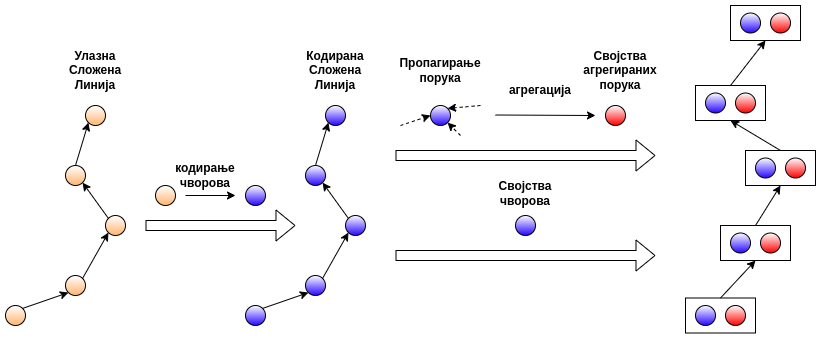
\includegraphics[width=0.9\textwidth]{images/vectornet-subgraph-rs.drawio.png}
  \caption{Визуализација једног слоја \label{vectornet-subgraph}}
\end{figure}

Из угла имплементације, улаз у ову компоненту модела је вектор димензије $B\times P\times T\times F$,
где је $B$ димензија подскупа података једног корака, 
$P$ је број сложених линија у једном графу, $T$ је дужина сложене линије, a $F$ је број својстава. Након $L$ слојева се добија вектор димензије 
$B\times P\times T\times (F \cdot 2^{L})$ који се агрегира на нивоу чворова на вектор димензије
$B\times P\times (F \cdot 2^{L})$\footnote{Претпоставка је да свака сложена линија има исти број својстава и да сваки граф има исти број сложених линија.}.
Агрегирану сложену линију посматрамо као један чвор у глобалном графу.
         
\subsection{Глобални граф интеракција}

Циљ глобалног графа интеракција је разумевање интеракција између агента и осталих објеката на сцени. Често постоји пуно објеката
на сцени, али агент не интерагује директно са свим тим објектима. Неопходно је да се издвоје објекти на сцени који су релевантни за агента.

Глобални граф интеракција се посматра као класичан граф са матрицом повезаности \textit{A}. Преко матрице повезаности \textit{A}
може да се дефинише хеуристика, као што је на пример удаљеност чворова на сцени. На тај начин се форсира да модел више узима у обзир ближе објекте
у односу на даље објекте на сцени.
У оригиналном раду се ради једноставности глобални граф посматра као потпуно повезан граф без тежина \cite{vectornet}.

Механизам пажње се примењује над
чворовима глобалног графа и проналазе везе између чворова графа \cite{attention_is_all_you_need}. Интуиција је да се на овај начин проналази путни сегменти који најбоље одговарају будућој трајекторији агента и
одређивање суседних објеката који утичу на само кретање агента. Не постоји ограничење на избор неуронске мреже која се примењује на глобални граф.
У наставку је дата општа формула глобалног графа интеракција. Глобални граф може да има више слојева, где
се векторизована репрезентација чвора $P_{i}$ ($i$ индекс тог чвора) у $l$-том слоју означава као $P_{i}^{(l)}$. 
Улаз у први слој глобалног граф интеракција је излаз подграфа из претходног корака, а векторске репрезентације тих чворова се означавају
са $P_{i}^{(0)}$.

\begin{figure}[H]
  \centering
  $\{P^{(l+1)}_{i}\} = GNN(\{P^{(l)}_{i}\}, A)$
\end{figure}

Конкретно у имплементацији се користи механизам пажње за \textit{GNN}.
Нека је $P$ матрица атрибута свих векторских репрезентација чворова поређаних у редове.
Векторске репрезентације се пројектују потпуно повезаним неуронским мрежама на $P_{Q}$ (упит), $P_{K}$ (кључ) и $P_{V}$ (вредност). 
Скалирање скаларног производа са $\frac{1}{\sqrt{d_{K}}}$ је опционо, где је $d_{K}$ број редова матрице $P_{K}$.

\begin{figure}[H]
  \centering
  $GNN = softmax(\frac{P_{Q}P^{T}_{K}}{\sqrt{d_{K}}})P_{V}$
\end{figure}

Глобални граф интеракција заједно са подграфом чини енкодер архитектуре,
чији је циљ разумевања контекста сцене на висиком нивоу. Последњи слој је декодер који се односи на предикцију трајекторија.

\subsection{Предикција трајекторија}

Излаз глобалног графа интеракција садржи векторске репрезентације за сваки чвор који одговара неком објекту на сцени.
За предикцију трајекторија се \textcolor{red}{филтрира} чвор тј. векторска репрезентација агента. За агента се примењује призвољан декодер модел
чији је излаз предикција трајекторије. Најједноставнији приступ је коришћење потпуно повезане неуронске мреже под претпоставком да су 
тачке трајекторије међусобно независне. Овај корак се замењује напреднијим приступом у модификованој верзији заснованој на узоркованим циљним тачкама.

\subsection{Функција грешке}

За функцију грешке предикције трајекторија $L_{traj}$ се користи Хуберова функција грешке тј. комбинација $L_1$ и $L_2$ функције грешке. Хуберова функција грешке $H_{\delta}$ се дефинише на следећи начин:

\begin{figure}[H]
  \centering
  $H_{\delta}(\hat{y}, y) = \begin{cases}
    \frac{1}{2}\cdot(y - \hat{y})^2, & |y - \hat{y}| \leq \delta \\
    \delta \cdot (|y - \hat{y}| - \frac{1}{2}\cdot \delta), & |y - \hat{y}| > \delta
  \end{cases}$
\end{figure}

У процесу тренирања може да се дода задатак \textbf{оцене недостајућих чворова глобалног графа интеракција} само у циљу
добијања боље генерализације модела. Насумично се бирају чворови у графу и замаскирају
се његова својства (множењем нулом).
Сваком чвору се додају две ,,нове`` вредности које су једнаке минималној вредности сваке од координата почетних
тачака сложене линије\footnote{Опис својстава сложених линија је описан у секцији за припрему података}. Нове вредности представљају репрезентације тих сложених линија који се користе као улази приликом тренирања модела за оцену недостајућих својстава чворова. Циљ овог задатка је форсирање бољег разумевања
веза између трајекторија и генерално веза између сложених линија у графу. Функција грешке овог задатка ($L_{node}$) се имплементира коришћењем $L_1$
функције грешке.

Функција грешке за оцену трајекторија агента $L_{traj}$ и функција грешке за оцену
недостајућих вредности чворова глобалног графа интеракција $L_{node}$ се сабирају у коначну функцију грешке \textit{VectorNet} модела.
Хиперпараметром $\alpha$ се додаје тежине једног сабирка функције грешке у односу на други \cite{vectornet}.

\begin{figure}[H]
  \centering
  $L = L_{traj} + \alpha \cdot L_{node}$
\end{figure}

\section{Модификована верзија \textit{VectorNet} са узоркованим крајњим тачкама трајекторија}

Претходно поменута верзија \textit{VectorNet} модела може да се унапреди додавањем доменског знања. Један приступ је да се користе унапред
дефинисани предлози трајекторија који се користе као основе за генерисање предикција трајекторија. Предлози су фиксни током процеса
предвиђања и бирају се на основу анализе података. Кластеровањем свих трајекторија се добија скуп типичних очекиваних праваца
који могу да се користе као основа приликом предвиђања \cite{multipath}.

Алтернатива која се исто заснива на предлозима је да се уместо предлога трајекторија користе предлози крајњих тачака трајекторија
тј. циљних тачака. Модел који генерише трајекторију на основу циљне тачке и својства из \textit{VectorNet} се тренира слично као и основни модел, 
али квалитет целог система доста зависи од квалитета узорковања тих предлога. Алгоритам за узорковање предлога је већ објашњен у секцији за
иницијалну припрему података.

Архитектура \textit{TNT: Target-driveN Trajectory prediction} \cite{tnt} се заснива баш на тој идеји. Њени кораци су следећи:
\begin{enumerate}
  \item Разумевање контекста помоћу \textit{VectorNet} модела (основа архитектуре);
  \item Генерисање корекција \textit(eng. offsets) и оцена поузданости за сваки предлог циљне тачке трајекторије;
  \item Узорковање модификованих предлога на основу оцењене поузданости;
  \item Оцена трајекторије до сваког изабраног предлога крајње тачке.
  \item Оцена вероватноће за сваку од добијену трајекторију;
  \item Филтрирање трајекторија на основу вероватноћа.
\end{enumerate}

На слици \ref{tnt-viz-1} су представљени кораци 2 и 3 под претпоставком да је корак 1 претходно извршен. На сцени се налазе два агента
\textit{1} и \textit{2}. Мали љубичасти кругови се односе на предлоге циљних тачака који су узорковани од кандидата путних сегмената у процесу припреме података.
Сви узорковани кругови се налазе на централним линијама путних сегмената, јер се тако узоркују. Кругови су означени тако да је јасно ком агенту припадају. На основу поузданости је 
извршено филтрирање иницијалних предлога, због чега су неки кругови избељени. За остале кругове постоје корекције\footnote{
  У имплементацији се у једном кораку генеришу корекција и поузданост за све узорковане циљне тачке, али овде су због прегледности
  избачене корекције за одбачене предлоге.
} (наранџасти кругови спојени са иницијалним предлогом).


\begin{figure}[H]
  \centering
  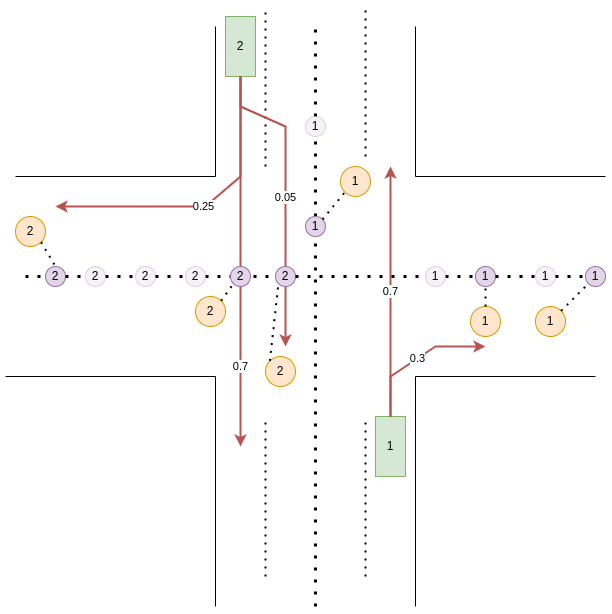
\includegraphics[width=0.6\textwidth]{images/tnt-viz-Page-1.drawio.png}
  \caption{Визуалиција \textit{TNT} - фаза 1 \label{tnt-viz-1}}
\end{figure}

На основу ових коначних циљних тачака се врши предвиђање трајекторија и то је приказано на слици \ref{tnt-viz-2}. Крај предвиђене трајекторије не мора
нужно да се поклапа са циљном тачком.

\begin{figure}[H]
  \centering
  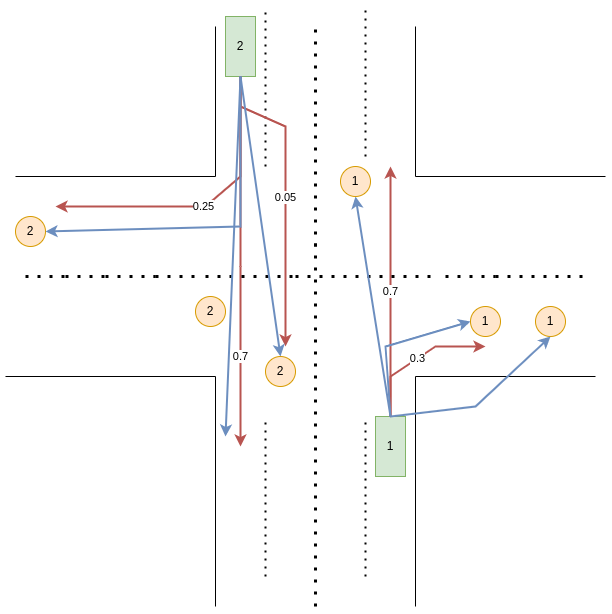
\includegraphics[width=0.6\textwidth]{images/tnt-viz-Page-2.drawio.png}
  \caption{Визуалиција \textit{TNT} - фаза 2 \label{tnt-viz-2}}
\end{figure}

Уместо последња два корака могу да се користе вероватноће (поузданости) предлога крајњих тачака (уместо целих трајекторија),
али из добре крајње тачке не следи
нужно квалитетна трајекторија (нпр. уколико предложена трајектрорија прелази преко тротоара). На слици \ref{tnt-good-target-bad-traj}
је дат такав пример. Овде је зелени правоугаоник агент, црвена трајекторија је истинита вредност трајекторије која се предвиђа, 
наранџасти круг је циљна тачка, а плава трајекторија је предикција. 

\begin{figure}[H]
  \centering
  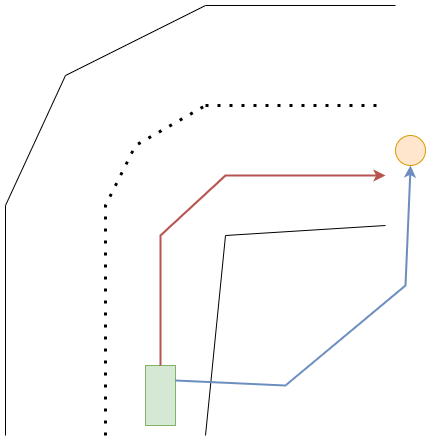
\includegraphics[width=0.5\textwidth]{images/tnt-good-end-point-and-bad-traj.drawio.png}
  \caption{Пример случаја где је добра циљна тачка, а лоша трајекторија \label{tnt-good-target-bad-traj}}
\end{figure}

\textit{VectorNet} чини језгро архитектуре, а сви наредни кораци могу да се имплементирају потпуно повезаним неуронским мрежама уз комбинацију
једноставних детерминистичких алгоритама. Главни изазов ове архитектуре је у алгоритму за генерисање 
предлога\footnote{Алгоритам је укратко описан у секцији за иницијалну припрему података} и балансирању
хиперпараметара функција грешака приликом учења модела.

Ако се не учи \textit{оцена недостајућих чворова глобалног графа интеракција} уз \textit{VectorNet},
онда функција грешке има следећи облик који ће бити објашњен у наставку:

\begin{figure}[H]
  \centering
  $L = \lambda_{1} \cdot L_{offsets} + \lambda_{2} \cdot L_{tarconf} + \lambda_{3} \cdot L_{trajde} + \lambda_{4} \cdot L_{trajconf}$
\end{figure}

Нека је $P_{p}$ скуп свих предлога крајњих тачака трајекторија и нека је $P_{gt}$ истинита крајња тачка трајекторије. Тада се издваја
из скупа $P_{p}$ елемент $P_{closest}$ који је најближи истинитој крајњој тачки\footnote{Овде не узимамо у обзир поправке,
већ нетрансформисане, узорковане вредности. 
Уколико се у обзир узимају вредности са поправкама, онда процес учења постаје тежак због шума (мења се индекс најближе тачке). Ово можда не би био
толики проблем да су остале трајекторије другачије дефинисане тј. независне од промене изабране, најближе тачке.}. 
Тада је:

\begin{figure}[H]
  \centering
  $L_{offsets} = H_{\delta}(P_{closest\_offset}, \hat{P}_{closest\_offset})$
\end{figure}

\noindent где је $H_{\delta}$ Хуберова функција грешке са параметром $\delta$, $P_{closest\_offset} = P_{gt} - P_{closest}$,
а $\hat{P}_{closest\_offset}$ је предикција тог одступања. Циљ је да баш тај најближи предлог има највећу поузданост, па се функција грешке за 
поузданост дефинише на следећи начин:

\begin{figure}[H]
  \centering
  $L_{tarconf} = BCE(P_{closest\_onehot}, \hat{P}_{confs})$
\end{figure}

\noindent где \textit{BCE} је бинарна унакрсна ентропија, $P_{closest\_onehot}$ индекс елемента $P_{closest}$ у \textit{onehot} 
формату\footnote{Индекс се представља као низ димензије броја класа (предложених крајњих тачака у овом случају) где су свуда нуле сем на локацији која одговара
вредности тог индекса.} и $\hat{P}_{confs}$ поузданост модела за сваки предлог (за сваки предлог се даје поузданост из интервала $[0, 1]$). Функција грешке за
трајекторије је аналогна као и за предлога крајњих тачака. Састоји се из функције грешке за одступање трајекторија од реализације и оцене
поузданости модела за сваку од тих трајекторија.

\begin{figure}[H]
  \centering
  $L_{trajde} = H_{delta} (T_{traj}, \hat{T}_{traj})$
\end{figure}

\noindent где је $T_{traj}$ истинита вредност трајекторије, а $\hat{T}_{traj}$ је њена предикција. Приликом предвиђања се
на основу предвиђених крајњих тачака оцењује трајекторија агента до тих тачака. Предикције крајњих тачака могу да варирају током процеса учења,
чиме се знатно отежава учење оцене трајекторије до крајње тачке због шума који настаје константном променом тежина у претходним слојевима.
Због тога се приликом учења за оцену трајекторије
$\hat{T}_{traj}$ узима истинита крајња тачка трајекторије како би учење било стабилније. Ова техника се зове ,,учитељско форсирање`` (\textit{eng. teacher forcing}) \cite{teacher_forcing}.

Последња компонента се односи на поузданост модела за сваку оцену трајекторија. За сваку оцењену трајекторију се рачуна максимално растојање
између свих упарених тачака оцењене трајекторије и истините вредности трајекторије тј.
$D(T_{traj}, \hat{T}_{raj}) := max(||T^{k}_{traj} - \hat{T}^{k}_{traj}||^{2}_{2})$. Тада се ,,истинита расподела`` $P_{traj\_confs}$ одређује као \textit{softmax} 
ових негативних вредности.

\begin{figure}[H]
  \centering
  $L_{trajconf} = BCE(P_{traj\_confs}, \hat{P}_{traj\_confs})$
\end{figure}

\section{Експерименти и резултати}

У табели \tref{vectornet-results} се налазе резултати \textit{TNT-VectorNet} модела. (TODO: Radim na poboljsanju rezultata)

\begin{table}[H]
  \begin{tabular}{c|c|c}
    Назив модела & \textit{minADE} (6) & \textit{minFDE} (6) \\
    \hline
    \textit{TNT-original без оцене трајекторија} & 0.877 & 1.632 \\
    \textit{TNT-original са оценом трајекторија} & 0.728 & 1.292 \\
    \textit{TNT-original-public} & 0.910 & 1.45 \\
    \textit{TNT-custom без оцене трајекторија}  & 1.19 & 2.25
  \end{tabular}
  \caption{Резултати}
  \label{vectornet-results}
\end{table}

Модел узима у обзир 50 узоркованих предлога за крајње тачке трајекторија агента и за сваки од тих предлога генерише корекције координата
и оцењује сваки од тих предлога. Филтрира се 12 најбољих од 50 крајњих тачака по оцени и за сваку од тих 12 крајњих тачака
модел естимира трајекторије заједно са њиховим естимираним вероватноћама. За крајњи резултат се бирају 6 трајекторије са највећим 
вероватноћама.   

На сликама \ref{tnt-MIA-210790} и \ref{tnt-MIA-36186} су приказа два сценарија и понашање модела тим сценаријима:
\begin{itemize}
  \item Сивом бојом су обојени путеви; 
  \item Тамно плавом је обојена историја трајекторија агента;
  \item Светло плавом су обојене историје суседних објеката;
  \item Црвеном линијом су обојени путеви кандидати;
  \item Мали љубичасти кругови су узорковани предлози;
  \item Велики плави кругови су изабрани узорковани предлози са највећом поузданошћу;
  \item Велики наранџасти кругови су модификовани изабрани предлози; 
  \item Светло зеленом бојом су представљене предикције за сваку од изабраних крајњих тачака;
  \item Тамно зеленом бојом су обојени истинити резултати. 
\end{itemize}

\begin{figure}[H]
  \centering
  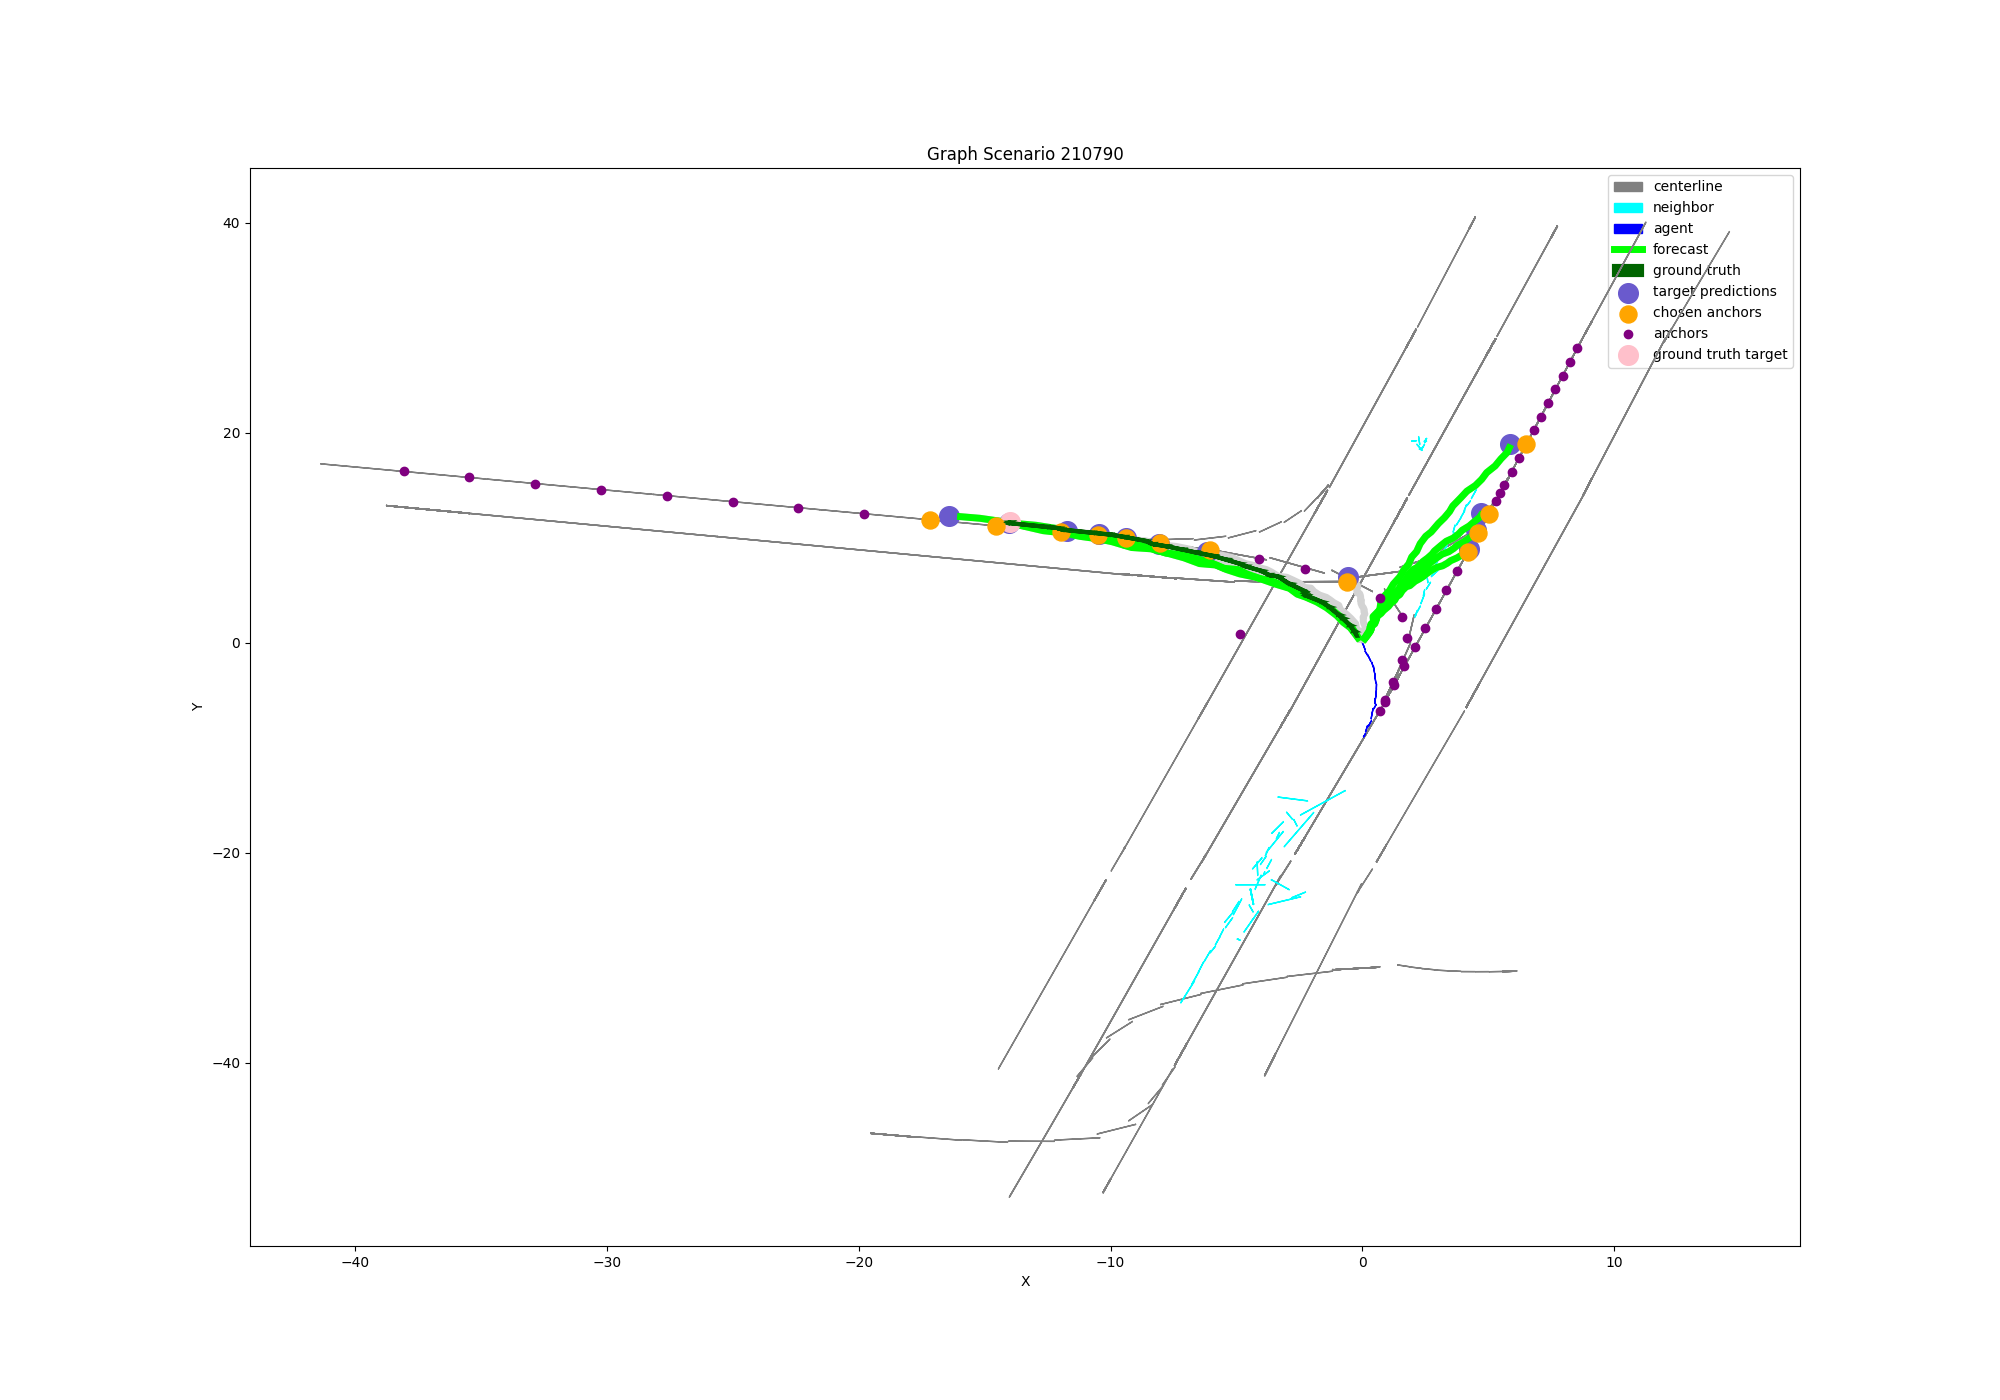
\includegraphics[width=0.9\textwidth]{images/result_MIA_210790_scenario.png}
  \caption{Предикције на сценарију \textit{MIA-210790} \label{tnt-MIA-210790} - TODO: legend}
\end{figure}

\begin{figure}[H]
  \centering
  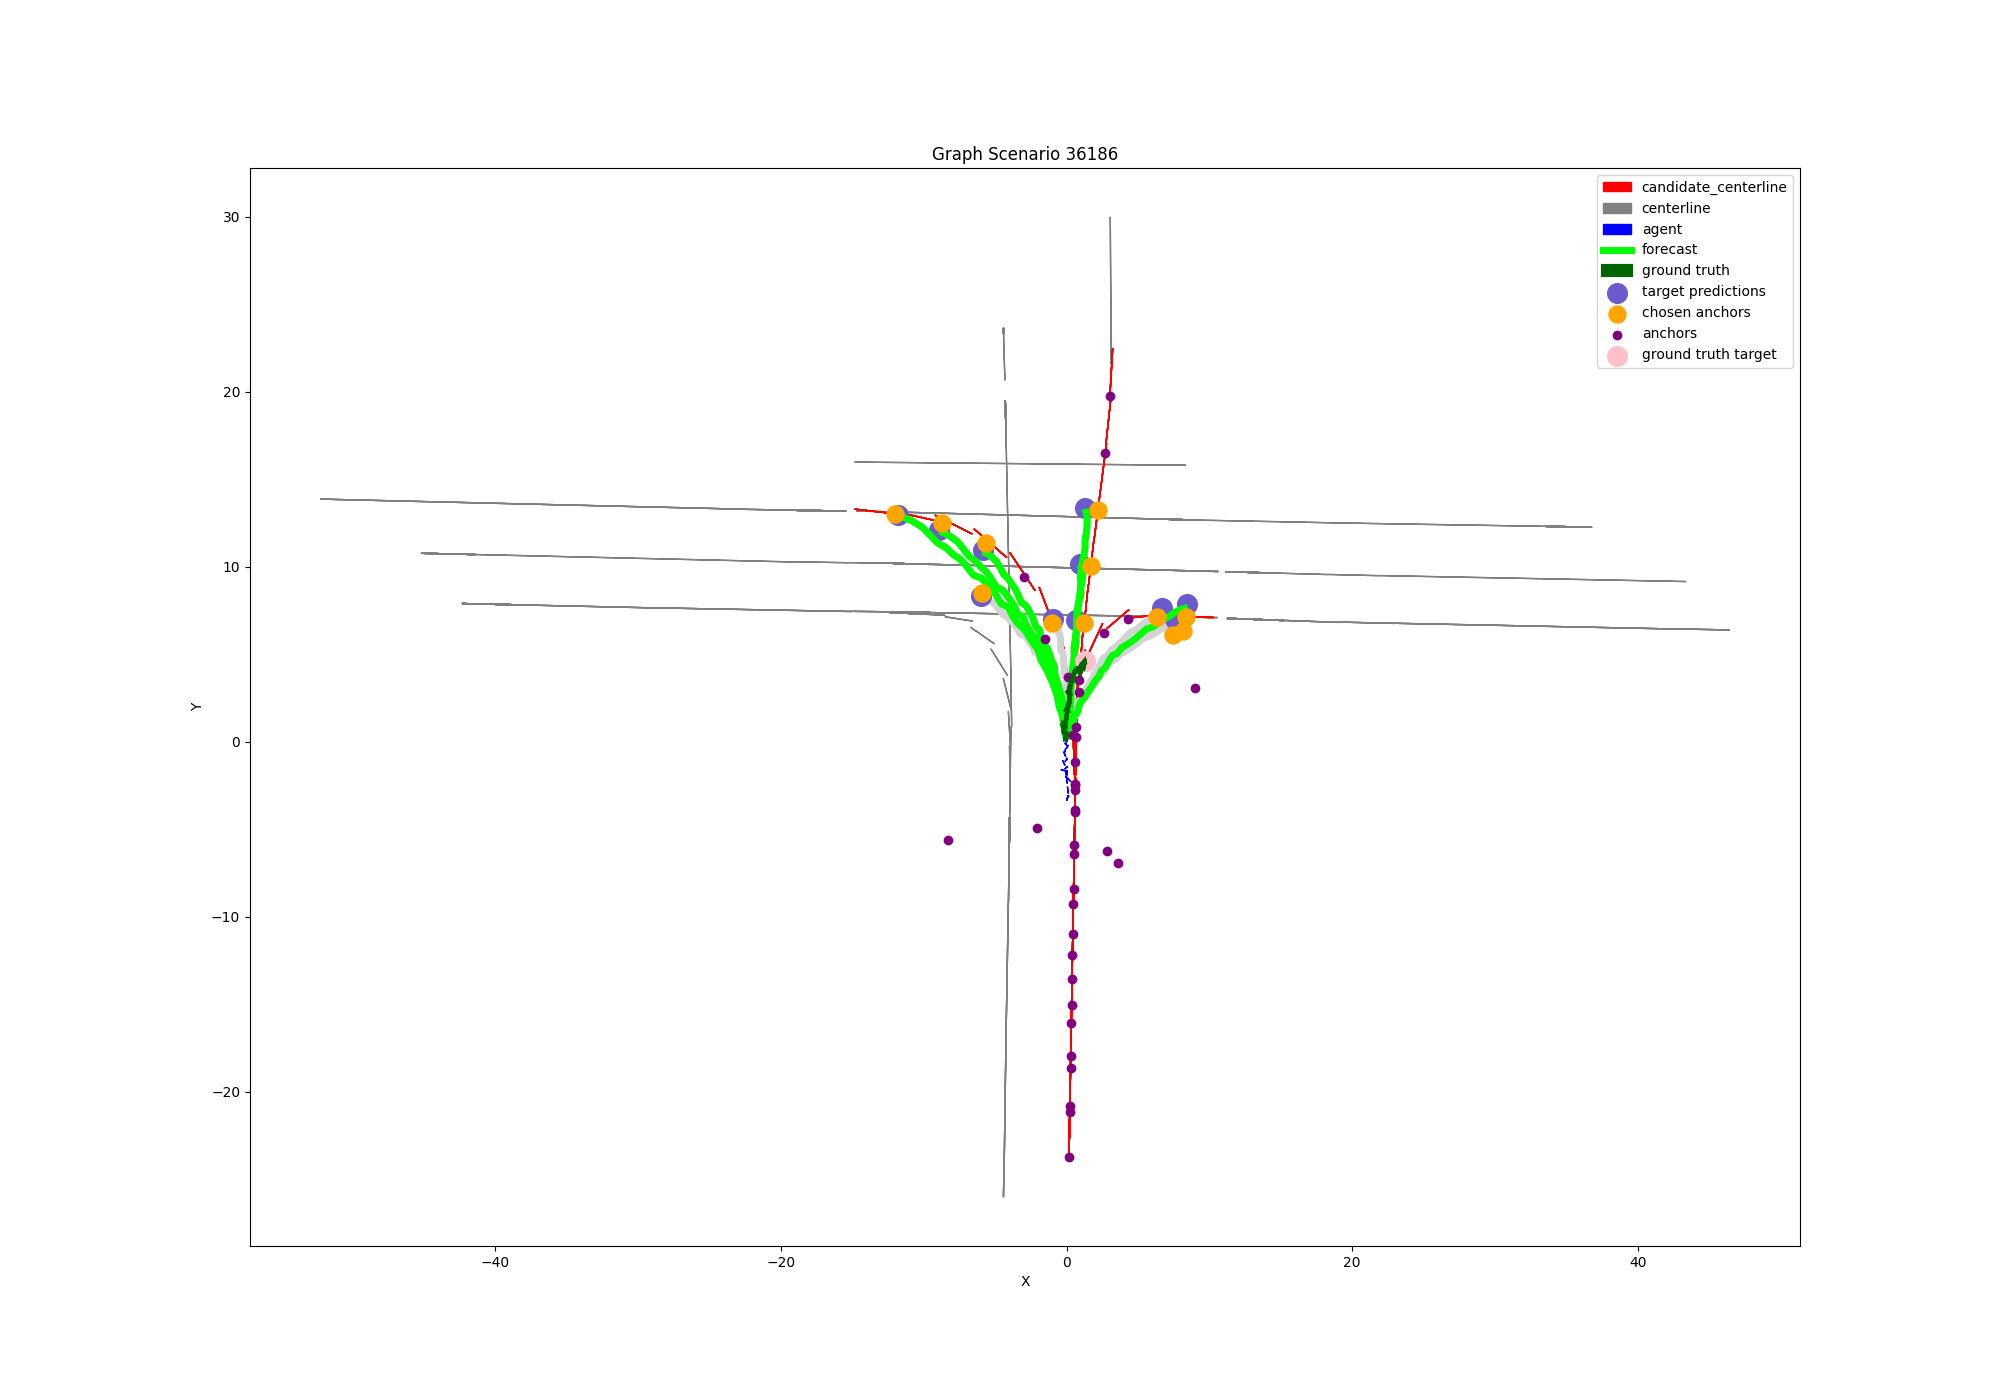
\includegraphics[width=0.9\textwidth]{images/result_PIT_36186_scenario.png}
  \caption{Предикције на сценарију \textit{MIA-36186} \label{tnt-MIA-36186} - TODO: legend}
\end{figure}

% ------------------------------------------------------------------------------
\chapter{Техника заснована на разумевању контекста обрадом растеризоване сцене}
\label{chp:razrada}
% ------------------------------------------------------------------------------

Алтернативни приступ структуирању података \textit{HD} мапа је растеризација. Како су подаци
сцене представљени из птичје перспективе тј. дводимензионалном облику онда је природно да се мапе сцена посматрају као слике. 
Уобичајно се слика представља као матрица пиксела, где сваки пиксел има једну вредност (један канал) у случају црно белих слика или 
три вредности (три канала) у случају слика у боји (нпр. \textit{RGB} формат). За \textit{HD}
мапе не постоје боје, већ се сваком пикселу додељују својства сцене. Неки од примера својства који могу 
да се доделе пикселу: да ли се на датој позицији налази агент,
да ли на тој позицији постоји контрола саобраћаја, да ли је могућа вожња на тој локацији и слично (конкретна својства
биће објашњена у следећој секцији). Избор својства која се додељују
пикселу је флексибилан и може да варира од једног скупа података до другог.
Процес трансформације \textit{HD} мапе у слику се у наставку реферише као растеризација \textit{HD} мапе. 

Када су подаци у облику слика, могућа примена конволутивних неуронских мрежа са циљем извлачења контекста сцене из растера. 
Контекст сцене се односи на све неопходне информације које модел користи за предвиђање трајекторија. Информације из контекста подразумевају
везу између агента и осталих објеката на сцени, везу између агента и путних сегмената, и одређивање простора у којем је агенту дозвољено да се креће.
Ове информације су комплексне и не могу се тек тако лако представити у векторизованом облику ручним издвајањем својстава. 
Претпоставка је да применом конволутивних неуронских мрежа могу извући информације на различитим нивоима комплексности. 

У овој глави се презентује постојећа архитектура \textit{HOME} која имплементира предикцију трајекторија у три фазе: 
генерисање топлотне мапе вероватноћа крајњих тачака трајекторије агента, 
узорковање крајњих тачака на основу претходно добијене топлотне мапе и оцена трајекторије до задате крајње
тачке \cite{home}. У наставку се прво описује припрема података. Након припреме података је детаљно описана архитектура.

\section{Растеризација \textit{HD} мапа}

Корак растеризације се наставља на иницијалну припрему у глави \ref{initprep}, исто као и припрема података за \textit{Vectornet} модел. 
Овај корак припреме захтева онлајн\footnote{Oнлајн припрема подразумева да се подаци припремају током тренирања модела.} 
приступ припреме због димензије података након конверзије у растеризовани облик. Растеризован облик чини
низ ретких матрица (већина вредности у матрици је нула), због чега подаци у том облику могу да буду 
и до 200 пута веће димензије од података у основном облику. За чување 
свих слика је потребно око \textit{4TB} за \textit{Argoverse} скуп података, 
док скуп података у основном облику заузима око \textit{30GB}. Иницијална
припрема, која претходи овом кораку, се и даље врши офлајн. 
Исти приступ је могуће искористити и за \textit{VectorNet} имплементацију, али у том случају није од толиког значаја. 

У \textit{Argoverse} скупу података су познате комплетне сцене градова, а за генерисање предикција конкретног агента у конкретном тренутку је
потребан само један исечак града у облику квадрата центриран у односу на агента. 
Димензија тог квадрата је хиперпараметар припреме података и модела. Квадрат је идеално довољно велики да обухвати скоро сваку
трајекторију у скупу података, али то захтева слике веће резолуције и самим тим је рачунски захтевније. 
За исечак се узима квадрат димензије $224\times 224$ центриран у односу на последњу познату локацију агента који обухвата
величину сваке трајекторије у скупу података. Центрирање се поклапа
са координатним системом агента у који се сцена пресликава у иницијалној припреми. Издвојен исечак са
одговарајућим својствима у сваком пикселу чини улаз у модел за генерисање топлотне мапе вероватноћа крајњих тачака агента. 

\subsection{Припрема улазних својстава}

Коначан облик једне слике је векторска репрезентација димензије 
$9\times 224\times 224$\footnote{Слика се представља у $C\times H\times W$ формату што одговара \textit{PyTorch} формату.}, 
где је $9$ број својстава додељених једном пикселу. Пример матрица сваког својства за конкретан сценарио се види на слици \ref{raster-MIA-24732}. 
Сваки пиксел садржи следећа својства:
\begin{itemize}
  \item Возно подручје: Да ли локација пиксела припада путу тј. да ли је могућа вожња на тој локацији. Информација се бележи бинарно, где
        1 означава да је на тој локацији могућа вожња, а 0 да није могућа вожња. Ово својство је јединствено за технике
        засноване на разумевању контекста растеризацијом сцене, јер такав податак није лако директно додати на граф. 
        Возно подручје је такође ротирано тако да одговара координатном систему агента.
  \item Растеризована трајекторија агента: Трајекторија агента се растеризује тако што се посматра локација агента
        у сваком тренутку који је забележен у историји трајекторије агента. За сваку локацију се одређује
        правоугаоник димензије $S_x\times S_y$ у њеној околини. 
        Сваки пиксел који припада том правоугаонику добија вредност 1 за својство растеризоване
        трајекторије агента, док вредност непромењених пиксела остаје на 0. 
        У оригиналној имплементацији се за сваки временски тренутак чува засебна матрица. То значи да се за трајекторију дужине 20 
        чува 20 веома ретких матрица. Ради уштеде ресурса се користи само једна матрица за све тачке трајекторије \cite{home}.
        Још једна алтернатива је да се на серију слика трајекторија примени \textit{ConvLSTM} мрежа као што је то урађено у \textit{CASPNet}
        раду \cite{caspnet}. 
  \item Растеризоване трајекторије суседа: Аналогно агенту се растеризују трајекторије осталих објеката на сцени.
  \item Растеризовани метаподаци путних сегмената: За сваки путни сегмент је дато 5 бинарних својстава:
        \begin{itemize}
          \item да ли путни сегмент припада пресеку путних сегмената;
          \item да ли путни сегмент обухвата контролу саобраћаја;
          \item да ли путни сегмент подразумева скретање удесно;
          \item да ли путни сегмент подразумева скретање улево;
          \item да ли путни сегмент не подразумева скретање.
        \end{itemize}
        Путни сегменти се посматрају као специјална врста трајекторија, па се растеризују аналогно трајекторији агента.
  \item Растеризовани кандидати путних сегмената: Кандидати путних сегмената на основу којих се узоркују предлози крајњих тачака
        за \textit{TNT-VectorNet} модел се у овом случају користе као улаз у модел. 
\end{itemize}

На слици \ref{raster-MIA-24732} је визуализованo свако од претходно наведних својстава. Белом бојом су обојени пиксели који имају вредност 1,
а необојени, црни пиксели имају вредност 0. 

\begin{figure}[H]
  \centering
  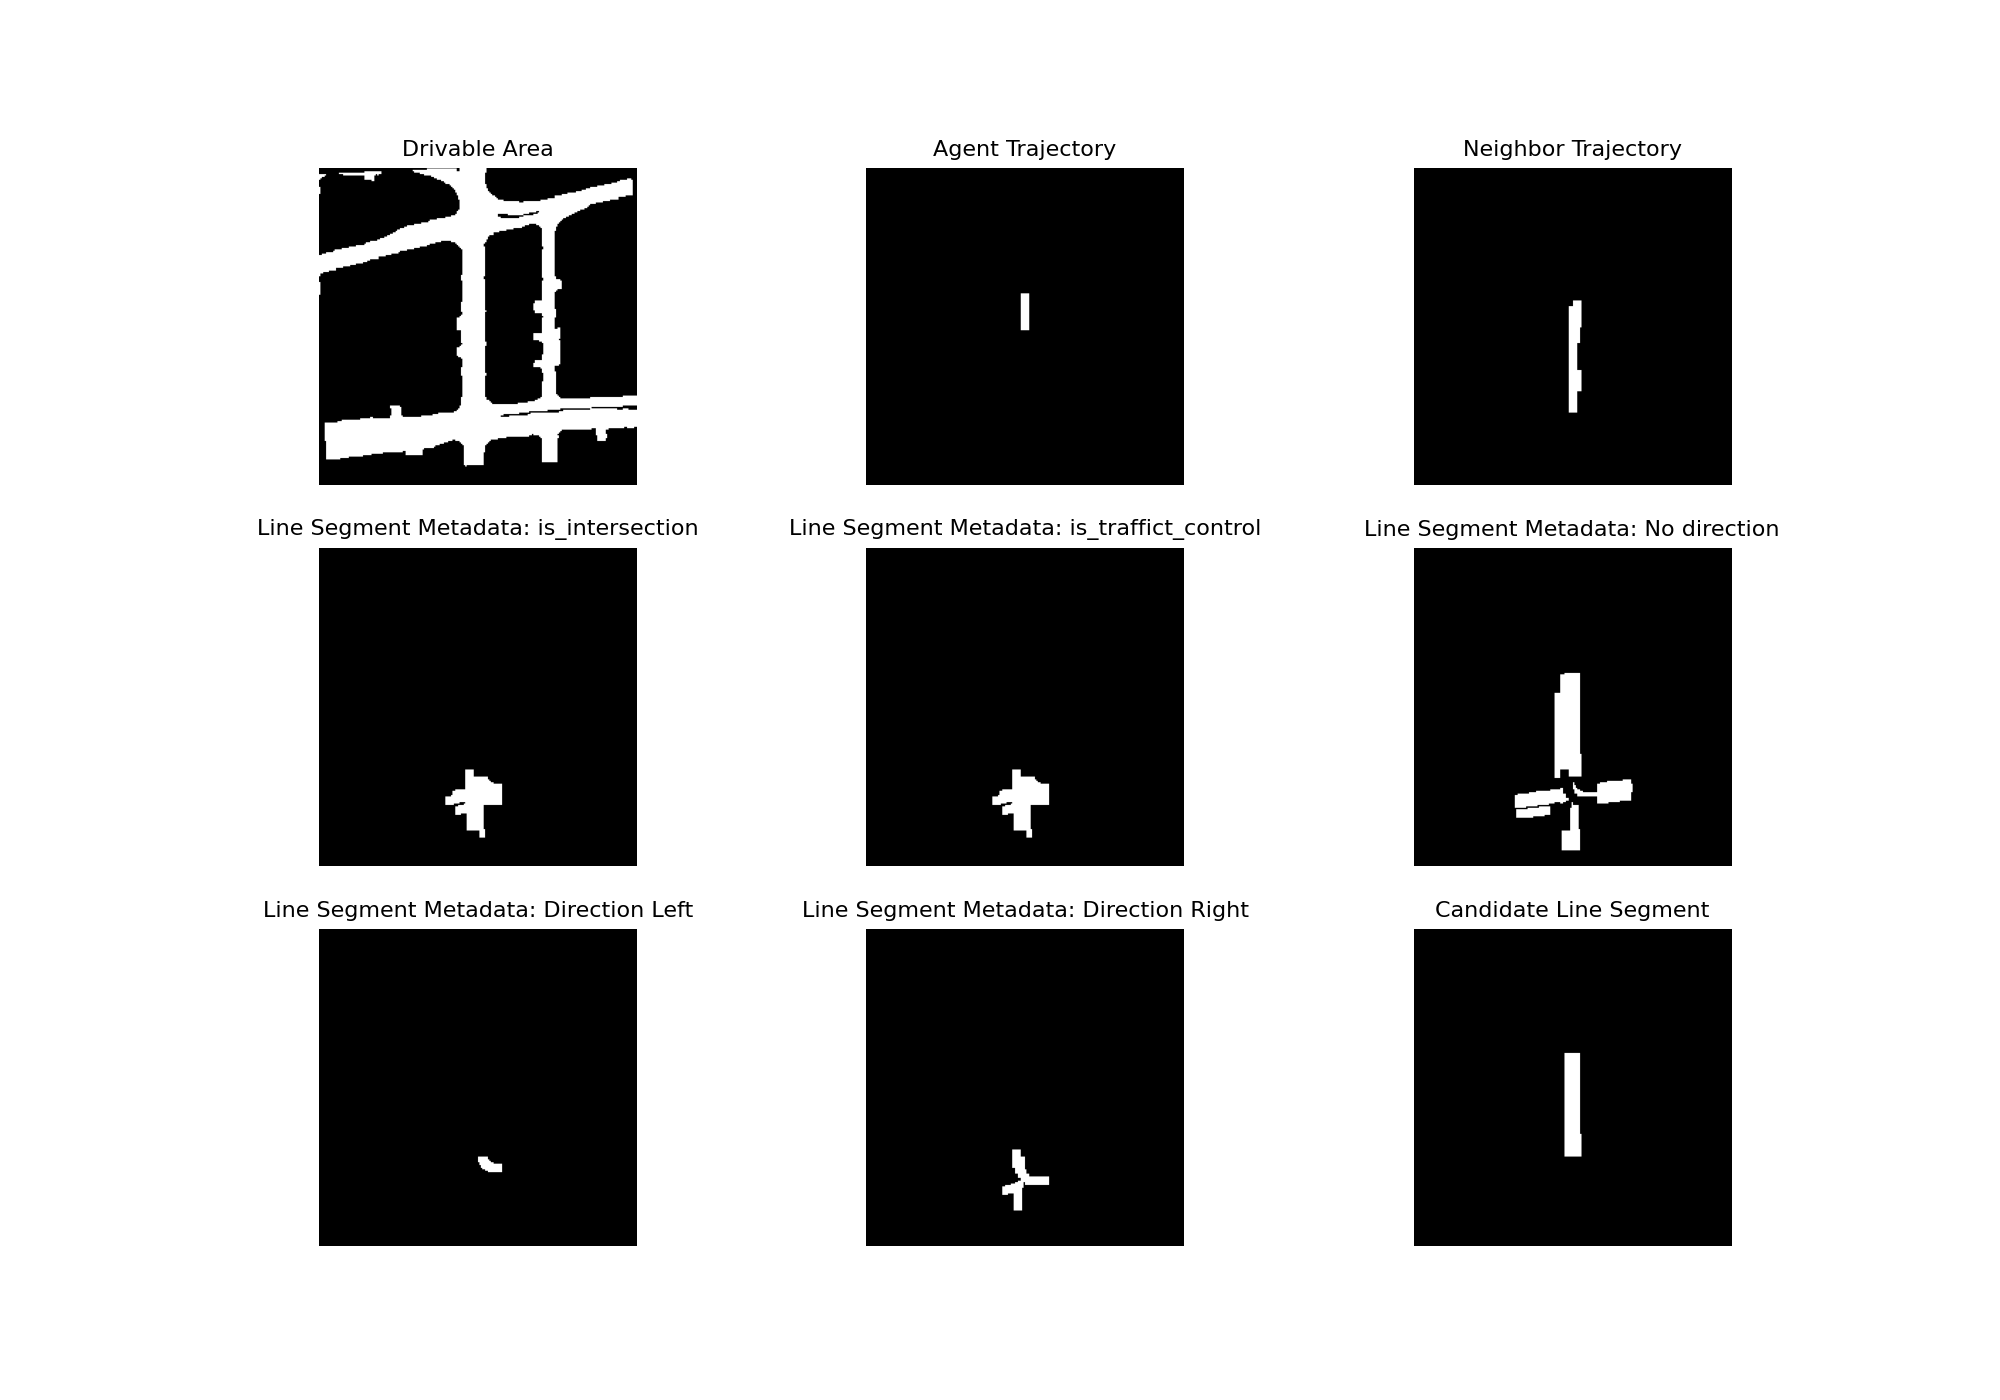
\includegraphics[width=1.0\textwidth]{images/raster_MIA_24732.png}
  \caption{Растеризована својства на сценарију \textit{MIA-24732} \label{raster-MIA-24732}}
\end{figure}

\subsection{Припрема топлотних мапа вероватноћа крајњих тачака агента}

Поред припреме улазних података у модел, припремају се и истините вредности топлотних мапа вероватноћа крајњих тачака агента. 
Истинита крајња тачка трајекторије агента припада тачно једном пикселу, али непосредно суседни пиксели такође чине добре предикције. 
У случају да се користи само један пиксел за истиниту вредност, модел се подједнако кажњава ако изабаре најгори могући пиксел 
за крајњу тачку агента као и када изабере пиксел који је непосредно поред истинитог пиксела. 
Како би се направила разлика између тих пиксела, примењује се Гаусов кернел након постављене истините крајње тачке топлотне мапе. 
Облик топлотне мапе је $224\times 224$ и поклапа се са димензијом улазне слике. 
Опционо, топлотна мапа која се добија као излаз модела може да буде мање димензије, а да се накнадно скалира на одговарајућу димензију. 

На слици \ref{heatmap-MIA-24732} је приказан пример сценарија са истинитом топлотном мапом. Црном бојом су обојени делови мапе
где није могућа вожња, а тамно сивом бојом су обојени делови мапе где је могућа вожња. Плава испрекидана линија представља историју
трајекторије агента, а зеленa испрекидана линија представља истиниту вредност трајекторије агента (део трајекторије који се предвиђа). Жутом бојом
је обојена топлотна мапа.

\begin{figure}[H]
  \centering
  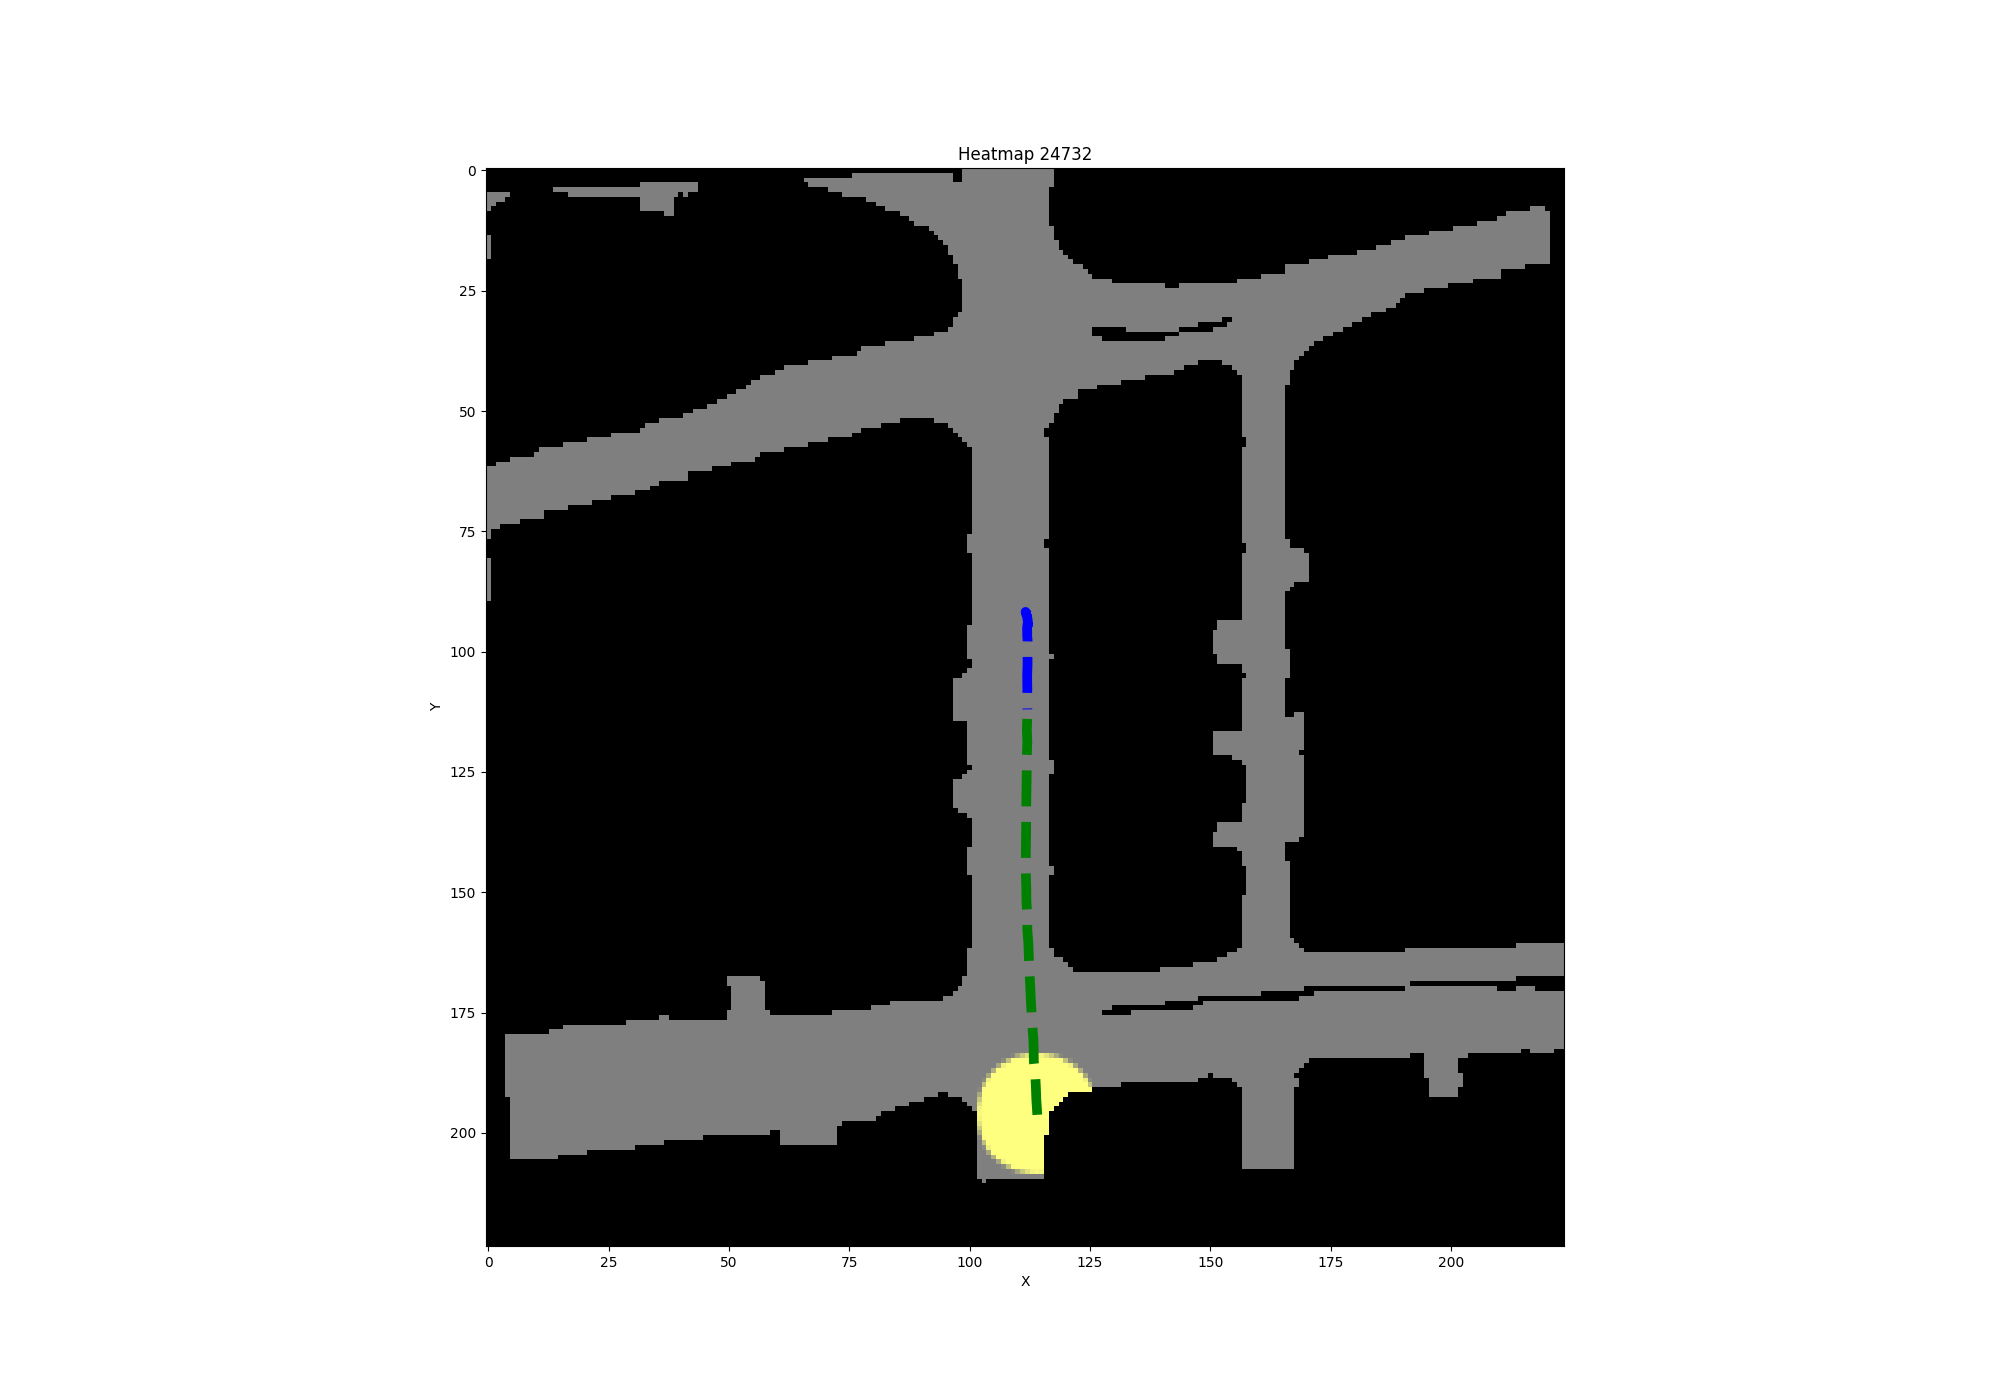
\includegraphics[width=0.9\textwidth]{images/heatmap_MIA_24732.png}
  \caption{Топлотна мапа крајње тачке трајекторије агента на сценарију \textit{MIA-24732} \label{heatmap-MIA-24732}}
\end{figure}

Архитектура \textit{HOME} поред слике користи и историју агента и осталих објеката у облику временских серија. Ове две структуре података
се комбинују.

\section{Модел \textit{HOME}}

Модел \textit{HOME (Heatmap Output for future Motion Estimation)} \cite{home} као улаз узима растеризовану слику сцене, историју трајекторије агента
и историју трајекторија суседа, 
а као излаз даје произвољан број предвиђених трајекторија за тај сценарио заједно са њиховим вероватноћама. 
Процес предвиђања се састоји из три корака који ће у наставку главе бити објашњени:
\begin{itemize}
  \item Генерисање топлотне мапе вероватноћа крајње тачке трајекторије агента;
  \item Узорковање крајњих тачака са топлотне мапе;
  \item Оцена трајекторије на основу узоркованих крајњих тачака.
\end{itemize}

Основна мотивација се поклапа са \textit{TNT-VectorNet} моделом тј. сматра се да ако се одреди крајња тачка трајекторије агента, онда применом једноставног
модела који узима у обзир ту крајњу тачку и историју трајекторије може тачно да се оцени трајекторија до те крајње тачке. Прва два корака се односе
на процес добијања крајњих тачака, а последњи корак се односи само на оцену трајекторија у случајевима када је позната крајња тачка трајекторије.

\subsection{Генерисање топлотне мапе вероватноћа крајње тачке трајекторије агента}

Прва фаза подразумева генерисање топлотне мапе вероватноћа крајње тачке трајекторије агента. Овај приступ је инспирисан \textit{CenterNet} \cite{centernet}
моделом за детекцију објеката на сликама. Укратко, идеја \textit{CenterNet} модела је да као излаз да топлотну мапу вероватноћа центара објеката тј.
сваком пикселу је додељена вероватноћа да се ту налази центар неког објеката. Узорковањем мода топлотне мапе се добијају центри објеката,
а одговарајући правоугаоници који обухватају објекат се добијају оценом ширине и висине. Аналогно том приступу, у случају предвиђања
трајекторија пикселима се додељује вероватноћа крајње тачке трајекторије уместо центра неког објекта на слици. 

Архитектура је енкодер-декодер, где се паралелно обрађују растеризована својства \textit{HD} мапе и својства историје трајекторија 
у основном (нерастеризованом) облику.
Обрада растеризованих својства одговара растер енкодеру тј. енкодеру статичког контекста сцене. Разумевање статичког контекста сцене се односи
на разумевање околине у којој се агент налази и ограничења која постоје на тој сцени као што су на пример валидни путеви и могућа скретања. 
Поред растер енкодера се користи енкодер историје трајекторија који одговара темпоралном енкодеру тј. енкодеру динамичком контексту сцене. 
Разумевање диманичког контекста се односи на разумевање динамике агента и интеракција са осталим суседима на сцени. 
Динамика агента се односи на његову брзину, смер, скретање и слично. 

Растер енкодер се састоји из низа конволутивних слојева и \textit{maxpool} операција. Конволутивним слојевима се издвајају
својства са сцене који се агрегирају \textit{maxpool} операцијом након које је димензија слике дупло мања по ширини и висини. 
Улаз у енкодер је је припремљен растер димензије $9\times 224\times 224$ на који се четири пута примењује пар конволутивног слоја и \textit{maxpool}
слоја што као излаз даје слику димензије $256\times 14\times 14$. У конволутивним слојевима се оквир матрице улаза проширује нулама (\textit{eng. padding}) 
тако да примена конволуције не утиче на димензију слике. Последњи слој растер енкодера је додатни конволутивни слој који даје слику димензије
$512\times 14\times 14$. \cite{home}

Основа за енкодер трајекторија је \textit{LSTM} рекурентна неуронска мрежа. Улаз у енкодер трајекторија је
историја трајекторије агента димензије $20\times 3$, 
где је 20 дужина историје трајекторије агента, а 3 је број својстава који садржи $x$ и $y$ координату заједно са информацијом да ли је тај 
временски тренутак допуњен (бинарна вредност) у случају да је оригинална дужина трајекторије била мања од 20. Аналогно се кодирају и
трајекторије суседа на сцени. Ради разумевања интеракција између агента и суседа, између њихових кодираних векторских репрезентација
се примењује механизам пажње, а излаз те операције се комбинује
са кодираном векторском репрезентацијом агента. Излаз векторске репрезентације енкодера трајекторија је димензије $128$
\cite{home}. 

Излаз растер енкодера и енкодера трајекторија се комбинују тако што се излаз из енкодера трајекторија понавља 14 пута по
ширини и дужини како би се добила
димензија $128\times 14\times 14)$. Овако добијен облик може да се налепи на излаз растер енкодера као додатни канали 
чиме се добија слика димензије $640\times 14\times 14$. Укратко, сваком пикселу се додају информације сцене добијене из енкодера трајекторија.

Спојени излаз два енкодера представља улаз у декодер који као излаз даје топлотну мапу димензије $224\times 224$ где сваки пиксел одговара
вероватноћи да се на тој локацији налази крајња тачка трајекторије агента. Декодер се имплементира као низ транспонованих конволутивних слојева
\cite{guide_to_cnn_arithm}, где сваки слој увећава димензију претходног улаза два пута по ширини и дужини. 
Слагањем 4 оваква слоја се добија излаз који је $16$ пута
већи по дужини и ширини и добија је жељена топлотна мапа димензије $224\times 224$. 
На крајњи излаз се такође примењује сигмоид функција $\sigma(x) = \frac{1}{1-e^{-x}}$ како би вредност сваког
пиксела припадала интервалу \textit{[0, 1]} тј. како би вредности излазa представљале валидне вероватноће које се моделују. 

\subsection{Функција грешке за генерисање топлотних мапа}

За учење се користи модификована фокална функција грешке \textit{eng. Focal Loss} 
инспирисана \textit{CenterNet} радом \cite{centernet, focal_loss}. Ова функција грешке
представља модификацију унакрсне ентропије која је погоднија у случају да се користи јако небалансиран скуп података између позадинских и непозадинских
класа. У основном облику, функција грешке унакрсне ентропије третира подједнако све негативне и позитивне узорке. 
У случају небалансираног скупа података, често постоји велики број лаких негативних примера који доминарају утицајем над градијентом
функције грешке током учења, што отежава сам процес учења модела. Стандардни облик функције грешке унакрсне ентропије је: 

\begin{figure}[H]
  \centering
  $ CE(\hat{p}, p) =
  \begin{cases}
    \centering
    -log(\hat{p}), & p = 1 \\
    -log(1-\hat{p}), & p \neq 1
  \end{cases}
  $
\end{figure}

Овде је $p$ лабела истините класа (0 за негативну и 1 за позитивну класу), а $\hat{p}$ је оцењена вероватноћа да је посматран узорак позитивна класа.
Фокална функција грешке додаје фактор $(1 - \hat{p})^{\alpha}$ за позитивну класу и фактор $\hat{p}^{\beta}$
за негативну класу, где су $\alpha$ и $\beta$ хиперпараметри. Општи облик фокалне функције грешке је \cite{focal_loss}:

\begin{figure}[H]
  \centering
  $ FL(\hat{p}, p) =
  \begin{cases}
    \centering
    -(1 - \hat{p})^{\alpha}\cdot log(\hat{p}) , & p = 1 \\
    -\hat{p}^{\beta}\cdot log(1-\hat{p}), & p \neq 1
  \end{cases}
  $
\end{figure}

На конкретном примеру је приказан ефекат фактора који се додају. Нека је $\alpha = 4,\ p = 1$. На слици \ref{fl-table} су приказане
вредности обе функције грешке за различите излазе модела. У случају великог броја лаких позитивних примера, очекује се да модел 
може врло брзо да научи да препознаје те позитивне примере и да буде веома сигуран приликом предвиђања тј. да вредности 
вероватноћа позитивне класе буду велике. Ти примери у случају фокалне функције грешке у даљем процесу тренирања имају мањи утицај
на вредности градијента (погледати последње редове у табели) у односу на стандардну функцију грешке унакрсне ентропије. 
Модел и даље наставља да учи над позитивним примерима које је класификовао нао негативне (погледати прве редове у табели).

\begin{figure}[H]
  \centering
  \begin{subfigure}{5cm}
    \begin{table}[H]
      \begin{tabular}{c|c|c}
        $\hat{p}$ & $CE(\hat{p}, 1)$ & $FL(\hat{p}, 1)$ \\
        \hline
        0.1 & 2.3026 & 1.5107 \\
        0.2 & 1.6094 & 0.6592 \\
        0.3 & 1.2040 & 0.2891 \\
        0.4 & 0.9163 & 0.1188 \\
        0.5 & 0.6931 & 0.0433 \\
        0.6 & 0.5108 & 0.0131 \\
        0.7 & 0.3567 & 0.0029 \\
        0.8 & 0.2231 & 0.0004 \\
        0.9 & 0.1054 & 0.0000    
      \end{tabular}
    \end{table}
  \end{subfigure}
  \begin{subfigure}{7cm}
    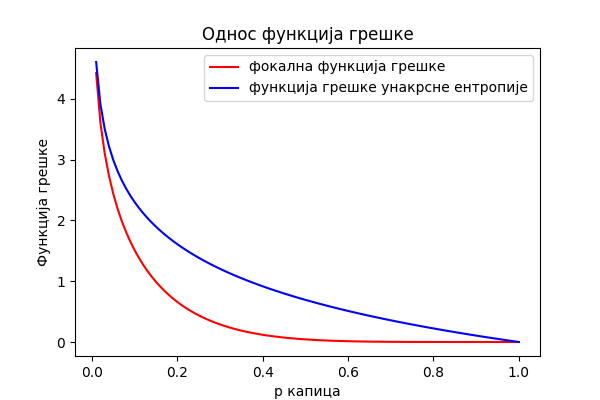
\includegraphics[width=1.0\textwidth]{images/fl_vs_ce.png}
  \end{subfigure}
  \caption{Анализа утицаја фокалног фактора на функцију грешке \label{fl-table}}
\end{figure}

У случају проблема генерисања топлотних мапа крајњих тачака трајекторија, постоји тачно један пиксел који одговара истинитој трајекторији
агента и који припада позитивној класи, док сви остали пиксели припадају негативној класи (нула пиксели). Ако је слика топлотне мапе димензије 
$224$x$224$, онда је однос позитивних и негативних класа
1 према 50176, што значи да је однос класа јако небалансиран. Такође, модел може врло лако у пар итерација да научи
да класификује већину нула пиксела тачно тј. постоји велики број лаких негативних класа. Ово је мотивација да се користи фокална функција грешка.

Функција грешке унакрсне ентропије и основни облик фокалне функције грешке дају исту вредност грешке за пиксел који је непосредно поред правог пиксела као и за
пиксел на слици који је најдаљи од правог пиксела. То није баш погодно јер пиксел који је непосредно поред правог пиксела такође 
представља јако добру предикцију за крајњу тачку трајекторије агента. 
Због тога се примењује Гаусов кернел ради ублажавања грешака у околини правог пиксела.
Вредност правог пиксела остаје 1.

Применом Гаусовог кернела над истинитом топлотном мапом се добијају "меке" класе тј. вредности су сада реални бројеви из интервала $[0, 1]$. 
Основна дефиниција фокалне функције грешке није погодна у том случају, јер је намењена за дискретне вредности 0 и 1. Архитектура \textit{HOME} користи
поједностављену верзију \textit{CenterNet} фокалне функције грешке и има следећи облик:

\begin{figure}[H]
  \centering
  $ FL_{home}(\hat{p}, p) =
  \begin{cases}
    \centering
    -log(\hat{p}) , & p = 1 \\
    -(1-p)^{4}\cdot log(1-\hat{p}), & p \neq 1
  \end{cases}
  $
\end{figure}

Смисао $(1-p)^4$ је умањивање грешке унакрсне ентропије у случају да је модел пикселима у околини правог дао вероватноће које су веће од 0.
Коначна функција грешке користи и средњеквадратно растојање:

\begin{figure}[H]
  \centering
  $ L_{home}(\hat{p}, p) = (p - \hat{p})^{2} \cdot
  \begin{cases}
    \centering
    -log(\hat{p}) , & p = 1 \\
    -(1-p)^{4}\cdot log(1-\hat{p}), & p \neq 1
  \end{cases}
  $
\end{figure}

\subsection{Узорковање крајњих тачака трајекторија}

Над добијеним топлотним мапама се примењује алгоритам за узорковање крајњих тачака трајекторија. Избор алгоритма у овом случају
је произвољан и може да се мења у зависности од метрике која се оптимизује. Алгоритам који је теоријски оптималан по \textit{FDE} метрици
не значи да је оптималан по \textit{MR} метрици и обрнуто. 

Произвољној трајекторији агента може да се додели вероватноћа користећи топлотну мапу крајњих тачака. Свакој трајекторији се додељује вероватноћа
као интеграл над порвршином која одговара околини крајње тачке на топлотној мапи. За околину може да се користи круг или квадрат са задатим 
полупречником. Посматрано из угла домена, круг има више смисла, али квадрат је погоднији јер одговара примени конволуције са филтером који има све јединице.
Примена филтера са свим јединицама је своди на сумирање свих вредности пиксела.
Ако је циљ оптимизација $MR^{\alpha}_{k}$ метрике, онда је то еквивалентно избору $K$ трајекторија тако да је збир вероватноћа 
тих трајекторија највећи \cite{home}. 
Проналазак оптималних $K$ тачака није лак проблем. Уместо тога може да се користи похлепни алгоритам који налази $K$ приближно оптималних
тачака. Похлепни алгоритам \ref{home-sampling-mr} је приказан у наставку.

\begin{figure}[H]
  \begin{python}
  def mr_uzorkovanje(t_mapa, k, radijus):
    # t_mapa: toplotna mapa
    # k: broj tacaka koje se uzorkuju
    # radijus: radijus okoline za aproksimaciju verovatnoce tacke

    suma_kernel = napravi_kernel_jedinica(radijus)
    traj_vrv = primeni_kernel(t_mapa, suma_kernel)
    
    tacke = []
    for _ in range(k):
      # pronalazak tacke sa najvecom vrv
      red, kolona = traj_vrv.argmax()  
      # brisanje okoline uzorkovane tacke
      # tj. postavljanje vrednosti piksela u okolini na 0
      traj_vrv = azuriraj_traj_vrv(traj_vrv, t_mapa, red, kolona, radijus)
      # koordinatni sistem se ne poklapa koordinatnim sistemom toplotne 
      # mape zbog primene konvolucije
      red, kolona = korekcija_koordinata(red, kolona, radijus)
      tacke.append((red, kolona))

    return tacke
  \end{python}
  \caption{Алгоритам за узорковање\label{home-sampling-mr}}
\end{figure}

Узорковане тачке се користе као улаз у модел за оцену трајекторија.
  
\subsection{Оцена трајекторије до предложене крајње тачке}

У овом тренутку се претпоставља да су дате крајње тачке трајекторија и да на основу њих треба да се оцене трајекторије. За оцену
трајекторија се користи једноставан модел који се састоји само од потпуно повезаних слојева. Над историјом трајекторије агента се
примењује потпуно повезан слој. Излаз тог слоја се спаја са координатама предложене крајње тачке, а након спајања се примењује још један
потпуно повезан слој којим се добија предвиђена трајекторија.

\subsection{Експерименти и резултати}

У табели \ref{heatmap-results} су приказане метрике из \textit{HOME} \cite{home} рада, као и метрике добијене
имплементације модификоване верзије тог модела. У табели
\ref{heatmap-results} је дато поређење оригиналног и имплементираног модела.

\begin{table}[H]
  \centering
  \begin{tabular}{c|c|c}
    Назив модела & \textit{minADE} (6) & \textit{minFDE} (6) \\
    \hline
    \textit{HOME-original} & 0.92 & 1.45 \\
    \textit{HOME-custom} & 1.04 & 1.93 \\
  \end{tabular}
  \caption{Резултати}
  \label{heatmap-results}
\end{table}

У наставку је издвојено неколико слика сценарија \ref{home-PIT-20617}, \ref{home-MIA-32197}, \ref{home-MIA-10454}, \ref{home-PIT-14577} 
који визуализују рад модела. На свакој слици сценарија је приказано возно подручје обојено тамно сивом бојом (није могућа вожња
у црним регијама), историја трајекторије агента обојена тамно зеленом бојом, реализација трајекторије агента обојена светло жутом бојом,
светло зелено област крајње тачке трајекторије агента која одговара истинитој топлотној мапи, означени пиксели предвиђене топлотне мапе
који имају веће вероватноће (област тих пиксела је обојена светло плавом бојом), предвиђење крајње тачке трајекторија агента
обојене црвеном бојом и предвиђене трајекторије агента обојене наранџастом бојом.

Прве три визуализација \ref{home-PIT-20617}, \ref{home-MIA-32197}, \ref{home-MIA-10454} представљају случајеве који су погодни моделу
и за које даје добре резултате. Модел за оцену трајекторија на основу крајње тачке трајекторије агента даје веома прецизне
предикције у случају да су те крајње тачке трајекторија агента смислене и прецизне. Пример \ref{home-PIT-14577} је издвојен као случај
где је модел узорковао три крајње тачке за оцену трајекторија агента које немају смисла, па су самим тим и оцењене трајекторије лоше.
Модел и даље скоро увек даје барем једну релативно прецизну крајњу тачку. Једна хеуристика која може да се примени без великих измена је да
се од скупа узоркованих тачака (неопходно је да се узоркује мало већи број тачака) је да се одбаце трајекторије које су већински нису на возном
подручју, па да се тек онда издваја $K$ трајекторија за које је модел најсигурнији.

\begin{figure}[H]
  \centering
  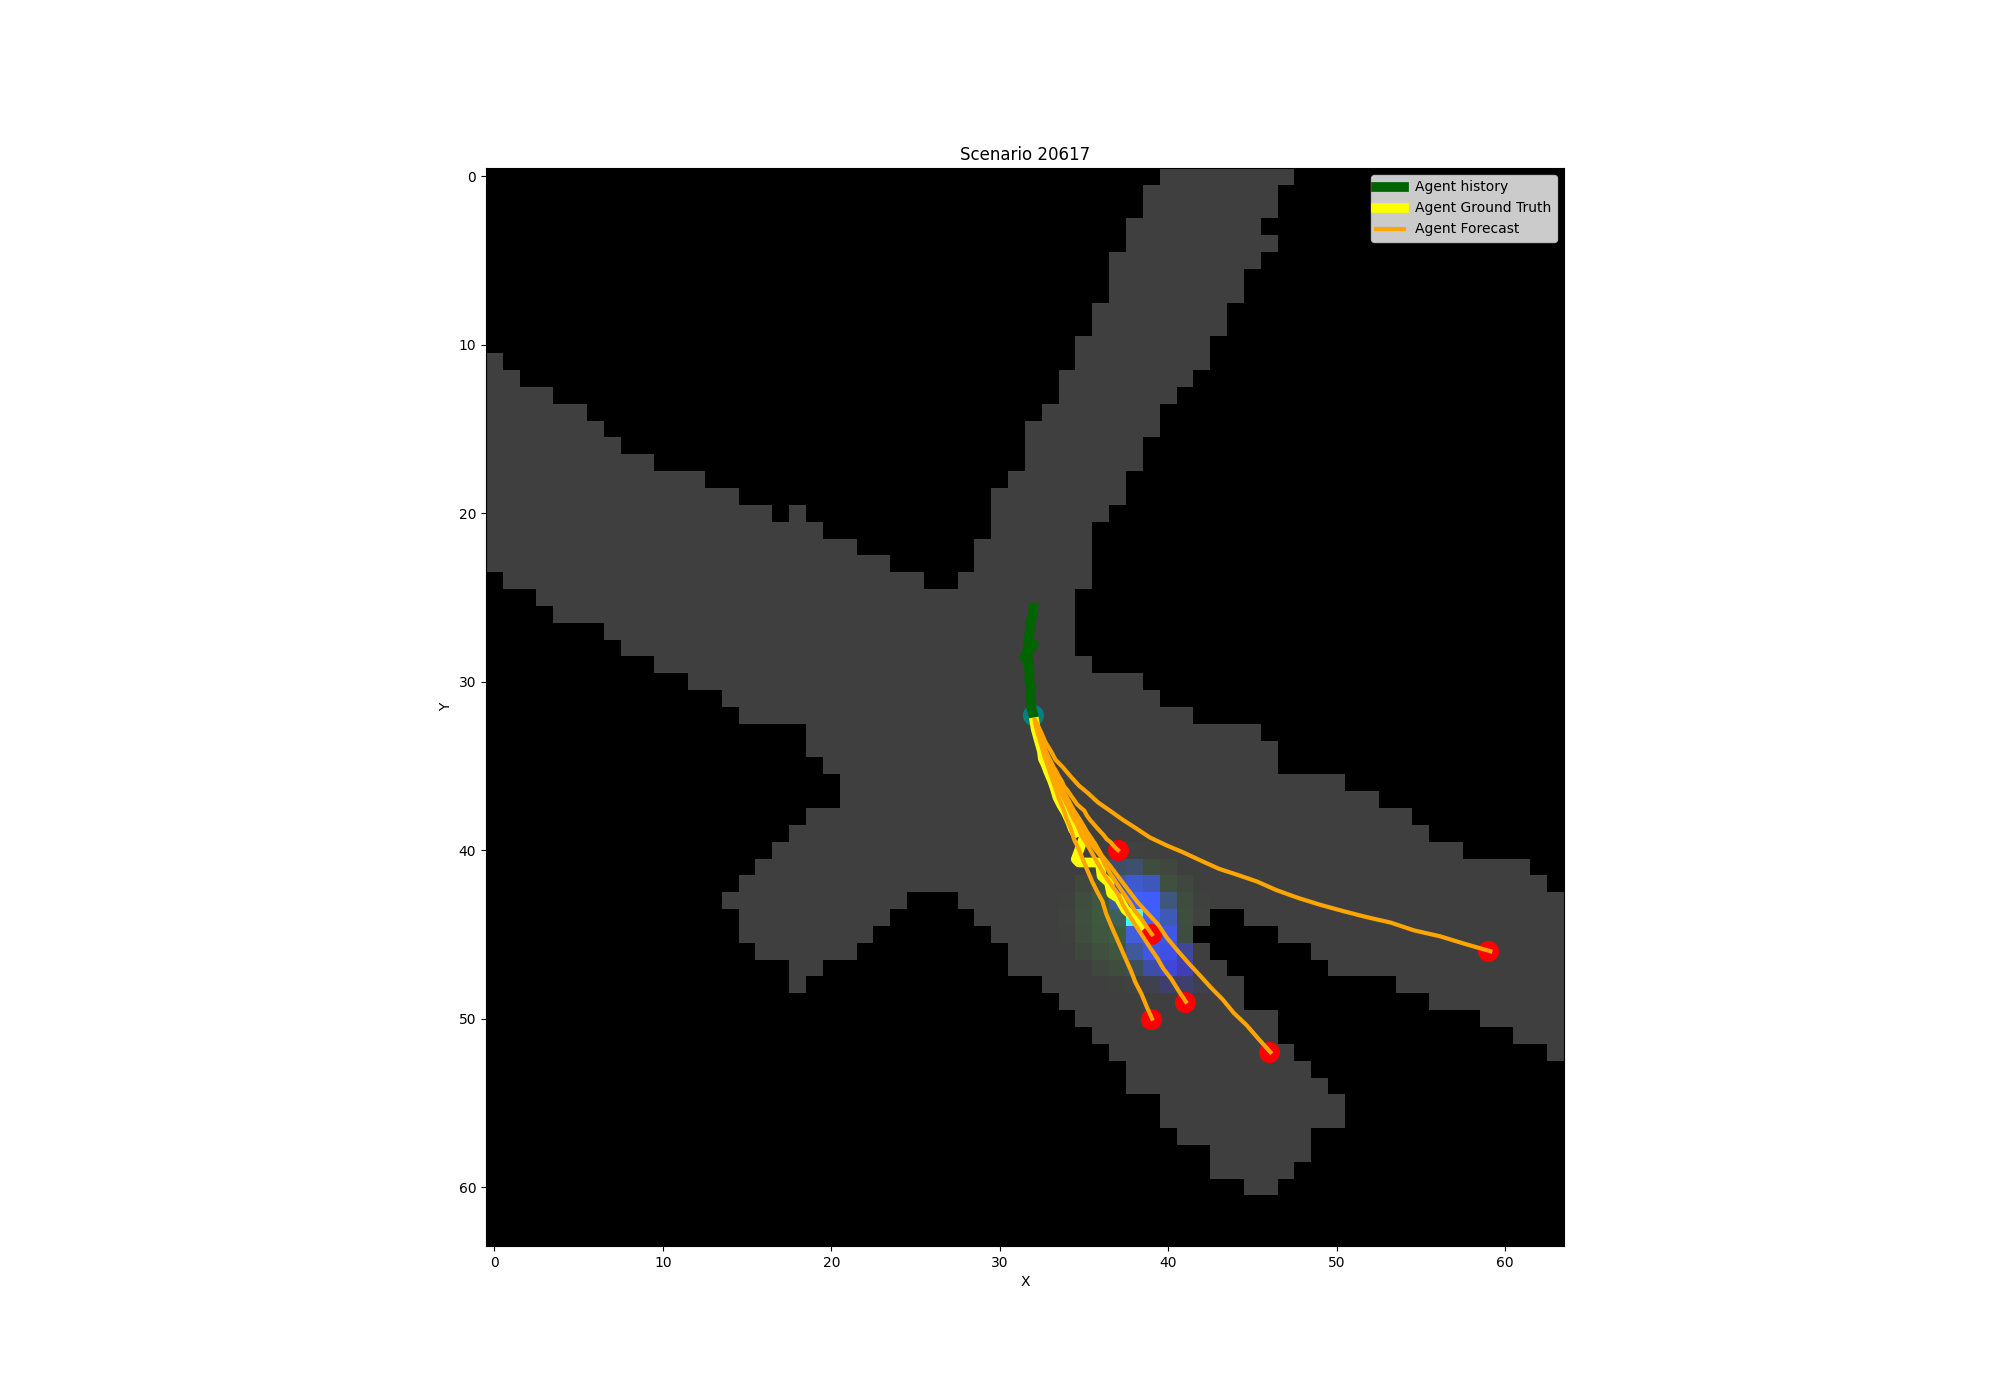
\includegraphics[width=1.0\textwidth]{images/home_PIT_20617.png}
  \caption{Резултати предикције \textit{HOME} модела - \textit{PIT-20617} \label{home-PIT-20617}}
\end{figure}

\begin{figure}[H]
  \centering
  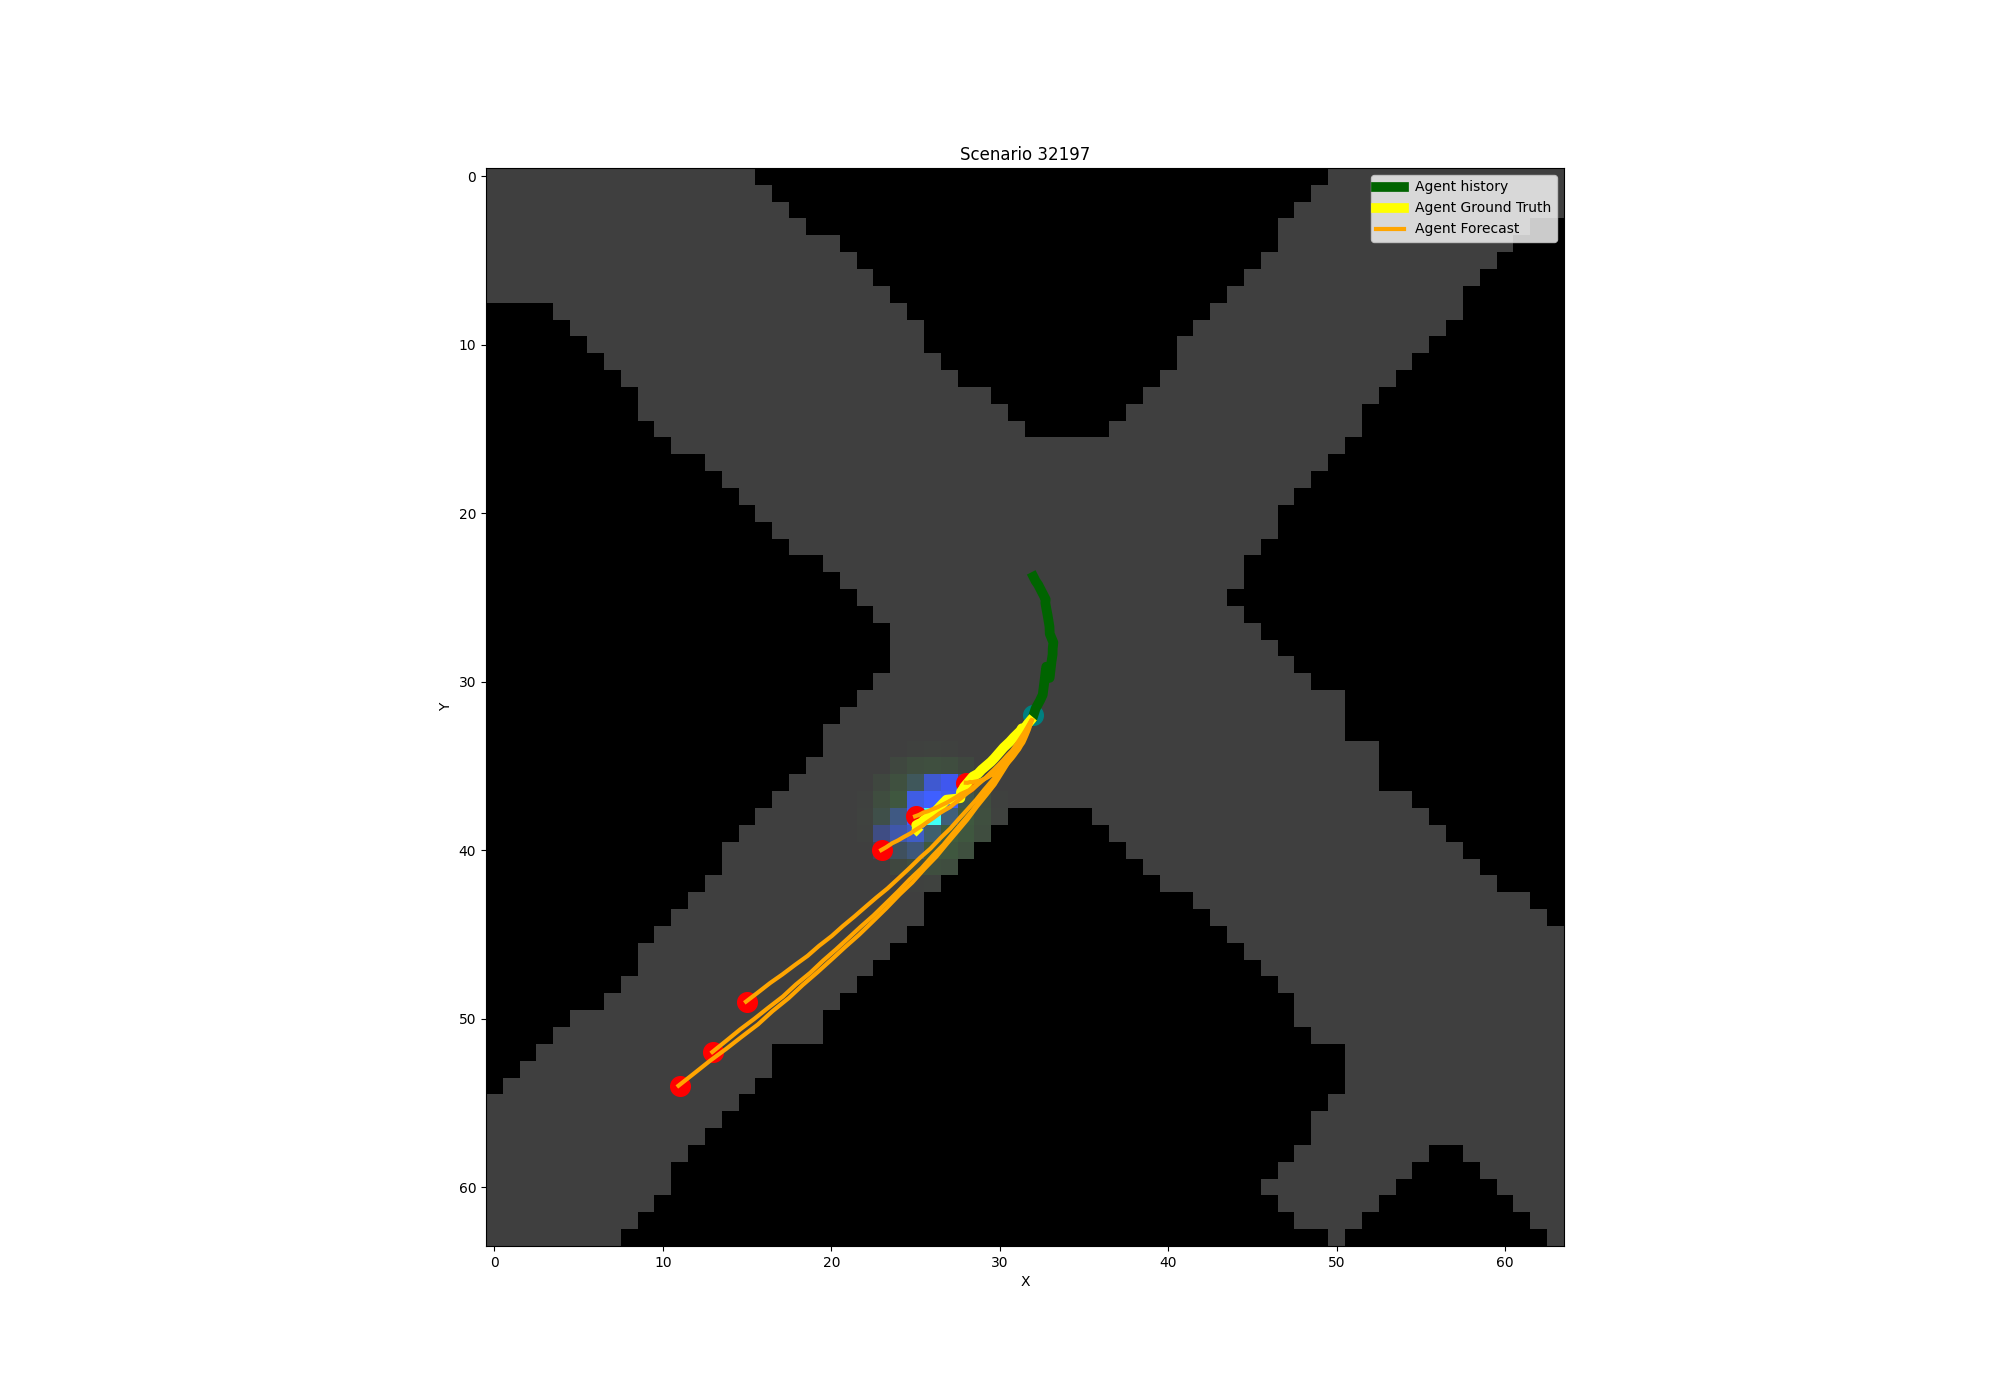
\includegraphics[width=0.8\textwidth]{images/home_MIA_32197.png}
  \caption{Резултати предикције \textit{HOME} модела - \textit{MIA-32197} \label{home-MIA-32197}}
\end{figure}

\begin{figure}[H]
  \centering
  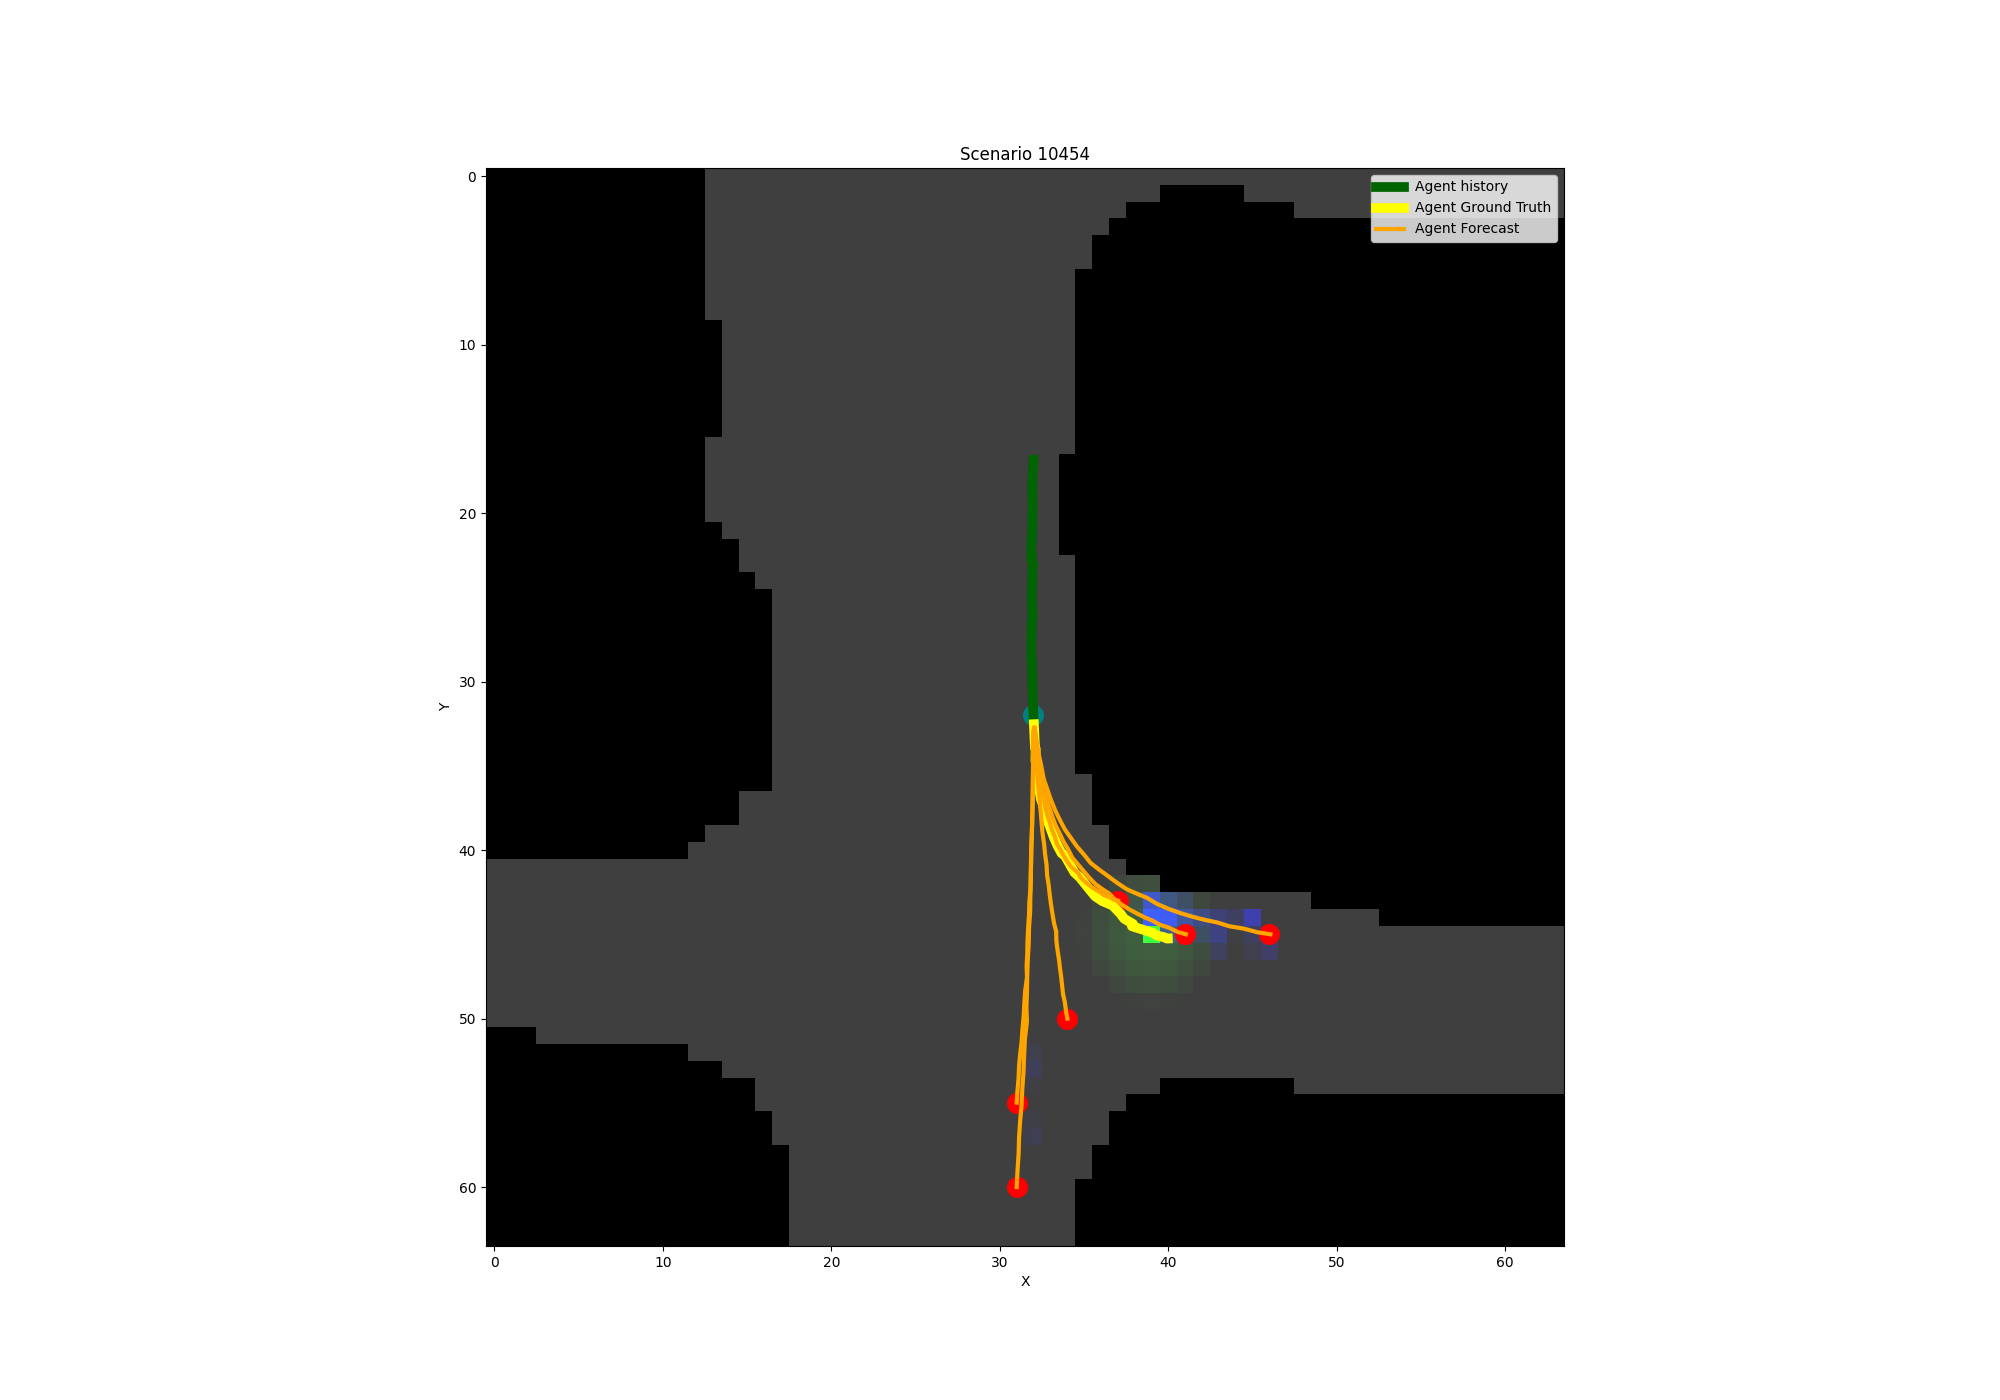
\includegraphics[width=0.8\textwidth]{images/home_MIA_10454.png}
  \caption{Резултати предикције \textit{HOME} модела - \textit{MIA-10454} \label{home-MIA-10454}}
\end{figure}

\begin{figure}[H]
  \centering
  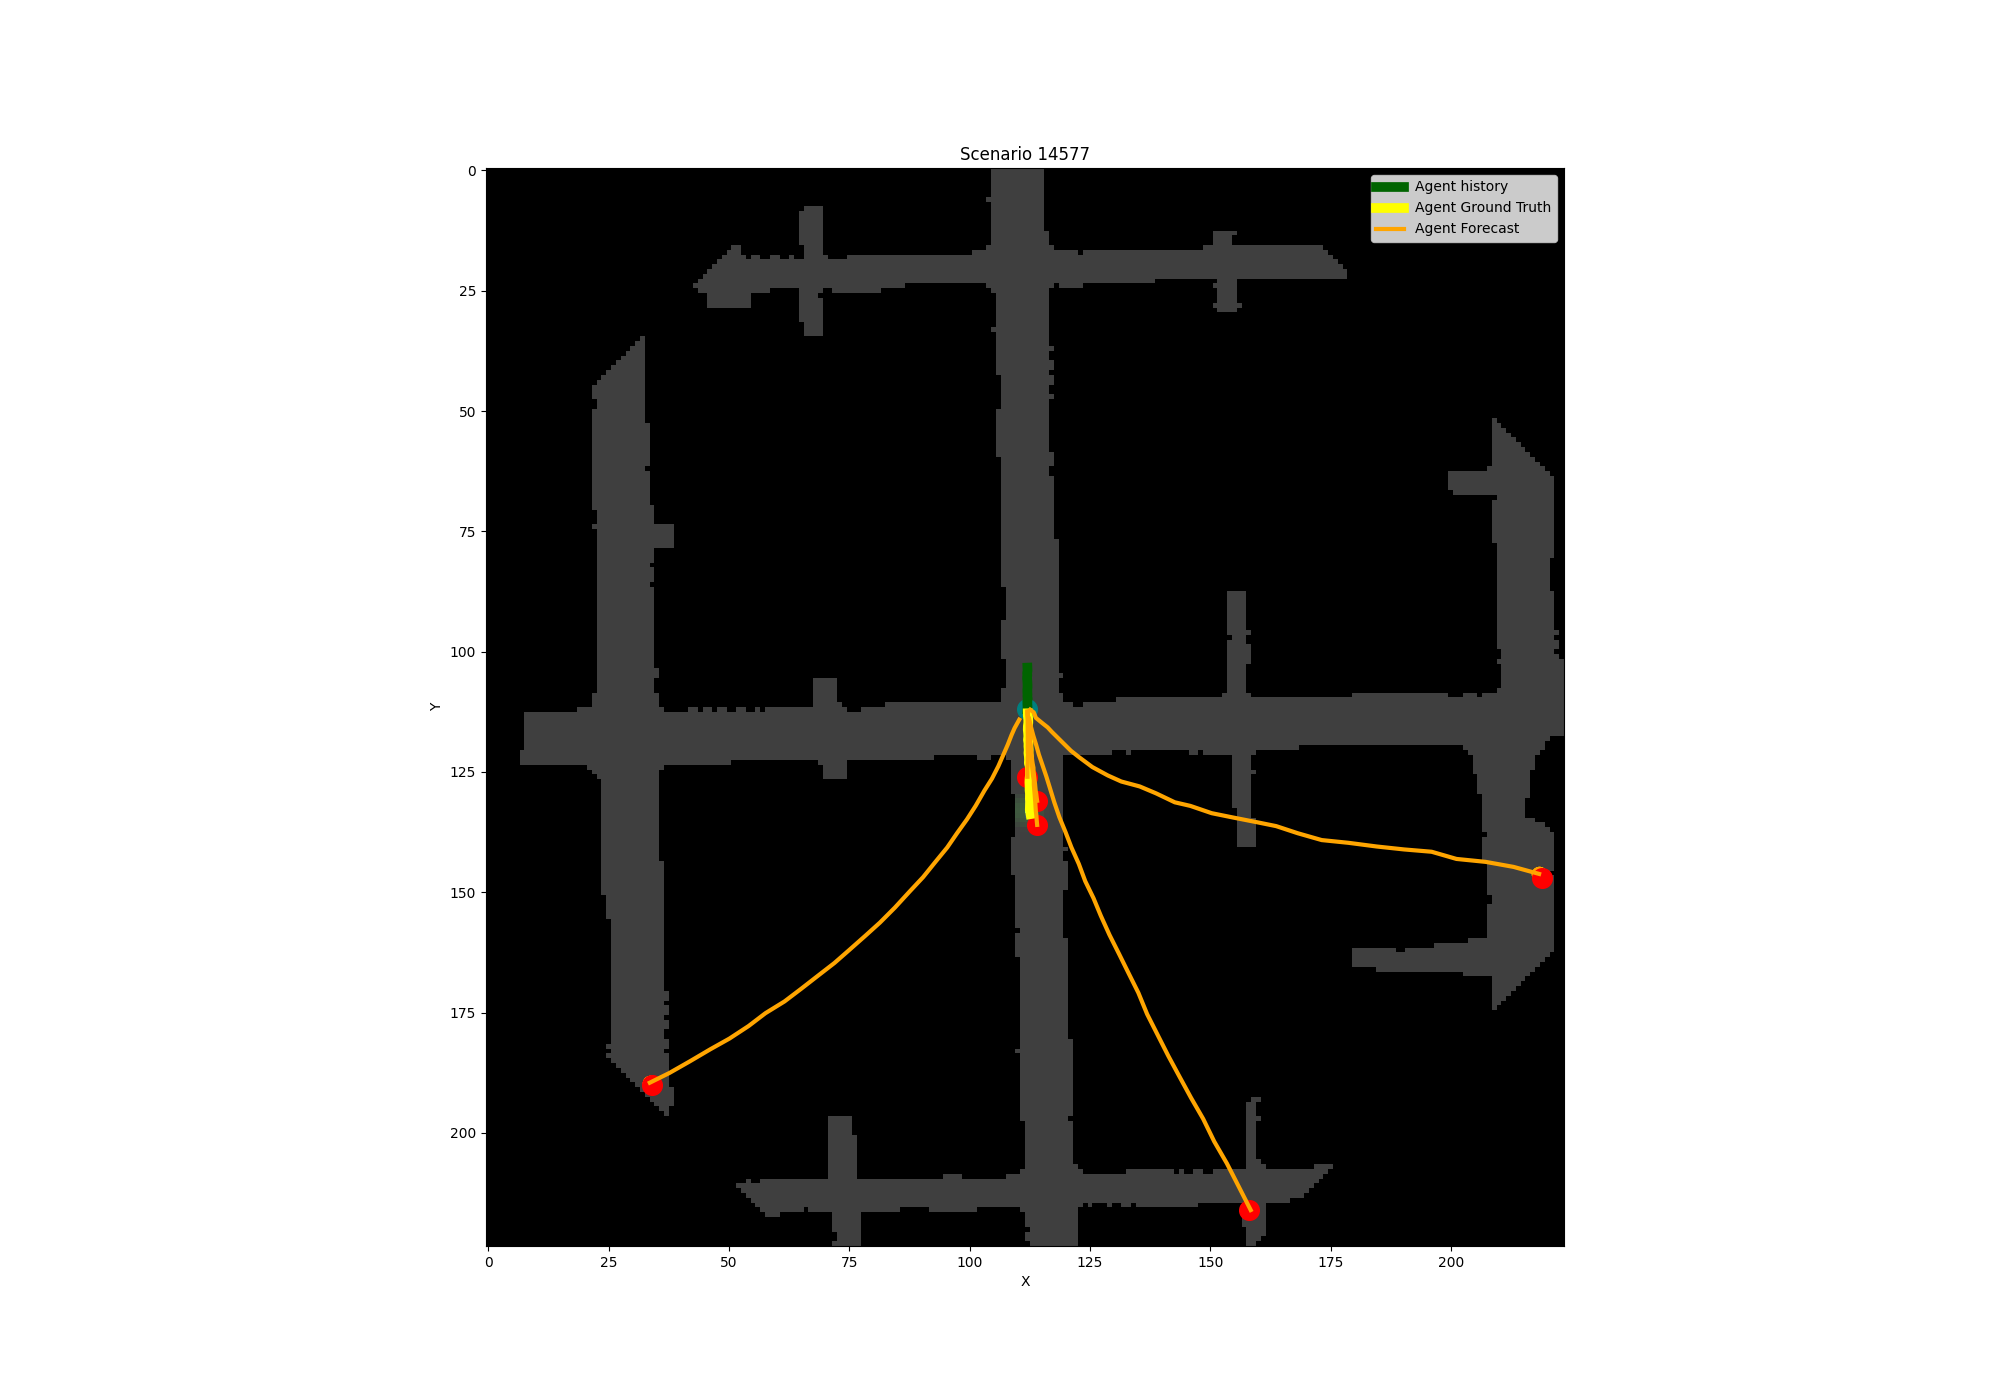
\includegraphics[width=1.0\textwidth]{images/home_PIT_14577.png}
  \caption{Резултати предикције \textit{HOME} модела - \textit{PIT-14577} \label{home-PIT-14577}}
\end{figure}

% ------------------------------------------------------------------------------
\chapter{Закључак}
% ------------------------------------------------------------------------------

У раду су имплементиране и анализиране две методе за предвиђање трајекторија за аутономну вожњу. 
То су \textit{TNT-VectorNet} модел (заједно са основним \textit{VectorNet} моделом) који је имплементиран као хијерархијска графовска неуронска мрежа
и \textit{HOME} модел који је имплементиран комбинацијом конволутивних и рекурентних неуронских мрежа. Ради поштеног поређења, оба
модела за учење и предвиђање користе исте информације тј. припрема података им се поклапа до тренутка конверзије у граф односно слику.

Предност приступа који раде са графовским структурама је у брзини модела током учења и предвиђања. Растеризацијом \textit{HD} мапа 
се драстично повећава димензија података без додавања нових информације, што додатно оптерећује хардверске ресурсе. У системима за аутономну
се упоредо извршава више задатака због чега су перформансе у реалном времену веома битне. Са друге стране, конкретна предност
\textit{HOME} архитектуре у односу на \textit{TNT-VectorNet} је могућност модела да научи да предвиђа своје предлоге крајњих тачака,
уместо да користи предлоге узоркованих на основу људских хеуристика. 

Компоненте ових архитектуре могу да се комбинују. Уместо растеризација \textit{HD} мапа за \textit{HOME} модел, може да се користи \textit{VectorNet}
као основа енкодера за генерисање топлотних мапа крајњих тачака. Тиме процес предвиђања постаје рачунски мање захтеван. Такође, предлози 
крајњих тачака узорковани из топлотних мапа \textit{HOME} модела могу да се користе као улази у \textit{TNT-VectorNet} без модификације
било које архитектуре.

% ==============================================================================
% Završni deo teze i prilozi
\backmatter
% ==============================================================================

% Datoteka sa literaturom u BibTex tj. BibLaTeX/Biber formatu
\bibliography{matfmaster-primer}
\bibliographystyle{ieeetr}

% ------------------------------------------------------------------------------
% Biografija kandidata
\begin{biografija}
\textbf{Момир Аџемовић} 
У изради...
\end{biografija}
% ------------------------------------------------------------------------------

\end{document} 
